% -*- TeX -*- -*- DE -*-

\chapter{PatchCore \cite{patchcore}}\label{ch:PatchCore}
\section{Einleitung}\label{sec:EinleitungPatchCore}
\textcolor{green}{\textit{Abgeschlossen: 01.11. v1}}\\
Die Methode \textbf{PatchCore} wurde erstmals am 15. Juni 2021 in Zusammenarbeit der Universität Tübingen und Amazon AWS im Paper \glqq Towards Total \ 
Recall in Industrial Anomaly Detection\grqq{} veröffentlicht. \ 
In seiner zweiten Fassung vom 5. Mai 2022 wurde das Paper bei der Konferenz CVPR 2022 (Computer Vision and Pattern Recognition) akzeptiert und zählt mit\ 
über 290 Zitierungen zu einem der populärsten Paper im Bereich der (Unüberwachten --> TODO) Anomaliedetektion.\\
Die Grundlage dieses Ansatzes sind wiederum \glqq Einbettungen\grqq{} (Embeddings) von Merkmalen (Feature), \ 
die aus den Eingabebildern mithilfe eines auf \glqq ImageNet\grqq{} vortrainiertem \glqq Convolutional Neural Network (CNN)\grqq{} erzeugt werden.\
Damit ähnelt sich die Methode PatchCore sowohl SPADE (\ref{sec:SPADE}), also auch PaDiM (\ref{sec:PaDiM}) und greift die in \ref{subsec:ResNetsAsFeatureExtractor} \
beschriebene Vorgehensweise auf.\
Wie wir später sehen werden, unterscheidet sich der Einbettungsprozess jedoch recht deutlich von den bisherigen Methoden.\
% Wie in einigen vorangegangenen Veröffentlichungen im Bereich der Unüberwachten Anomaliedetektion, werden auch hier die Features in \glqq Patches\grqq{} \ 
% unterteilt, um die Lokalität der Anomalien zu erhalten. Diese werden folgend als \textbf{\glqq Patch Features\grqq{}} bezeichnet.\
Weiter wird die eigentliche Anomaliedetektion, wie bereits bei der Methode SPADE mithilfe einer Nächsten Nachbar Suche \ 
(Nearest Neighbor Search; NN) in einer \glqq Memory-Bank\grqq{} $\mathcal{M}$ durchgeführt.\
Die wesentliche Weitereentwicklung gegenüber SPADE liegt vor allem in der Methode, wie die Memory-Bank aufgebaut wird. Durch die Auswahl möglichst representativer \
Elemente in der Memory Bank, kann die Anzahl der Elemente in der deutlich reduziert werden, was einer Reduzierung der Laufzeit bedeutet.\\
Auch gut 2 Jahre nach Veröffentlichung ist die PatchCore Methode insbesondere auf dem MVTecAD-Datensatz (\ref{sec:DatensatzMVTecAD}) mit einer Genauigkeit (Auccuracy) \ 
von maximal \num{99,6}\% (\glqq PatchCore Ensemble\grqq{}) absolut konkurrenzfähig und wird in vielen Veröffentlichungen als \glqq State-of-the-Art\grqq{} Methode verwendet.\\
Im Laufe dieses Kapitels soll zunächst die Funktionsweise der Methode PatchCore erläutert werden. Anschließend evaluieren wir die Originalmethode im Hinblick auf Laufzeit und Genauigkeit. \
Im sich dann anschließenden Teil werden zahlreiche Modifikationen besprochen, die versuchen, die Laufzeit auf zu Reduzieren und dabei möglichst viel der Genauigkeit zu erhalten.\
\section{Funktionsweise}\label{sec:FunktionsweisePatchCore}
\textcolor{green}{\textit{Abgeschlossen: 01.11. v1}}\\
Zunächst kann zwischen zwei Phasen unterschieden werden: Der Trainingsphase und der Testphase.\
In der Trainingsphase werden die \glqq (locally aware) \textbf{Patch Features}\grqq{} aus den Trainingsbildern (\glqq Nominal Samples\grqq{}) extrahiert. \ 
Hierzu wird ein \glqq Pretrained Encoder\grqq{} verwendet, analog zu \ref{subsec:ResNetsAsFeatureExtractor}.\
Anschließend findet eine Unterabtastung bzw. eine Auswahl der Patch Features statt, die in der Memory Bank gespeichert werden. \ 
Dieser Vorgang wird als \glqq Coreset Subsampling\grqq{} bezeichnet. Ist diese Memory Bank erzeugt, ist die Methode initialisiert und das Training abgeschlossen.\ 
In der Testphase werden die Patch Features auf die gleiche Weise aus den \glqq Test Samples\grqq{} extrahiert, wie in der Trainingsphase. Jedes dieser Patch Features wird nun mit den Patch Features in der Memory Bank verglichen.\
Dies geschieht mit einer \glqq Nearest Neighbor Search\grqq{} (NN). Aus den Distanzen zum Nächsten Nachbarn kann dann, wie in \ref{sec:PaDiM} eine räumlich aufgelöste Anomaliekarte erzeugt werden.\
Auf Grundlage dieser Anomaliekarte geschieht dann die Instanzklassifizierung als nominales oder anomales Bild. Nachfolgende Abbildung (\ref{fig:PatchCore}), die aus der Veröffentlichung übernommen wurde, zeigt \
die Funktionsweise der Methode PatchCore.\
\begin{figure}[h]
    \centering
    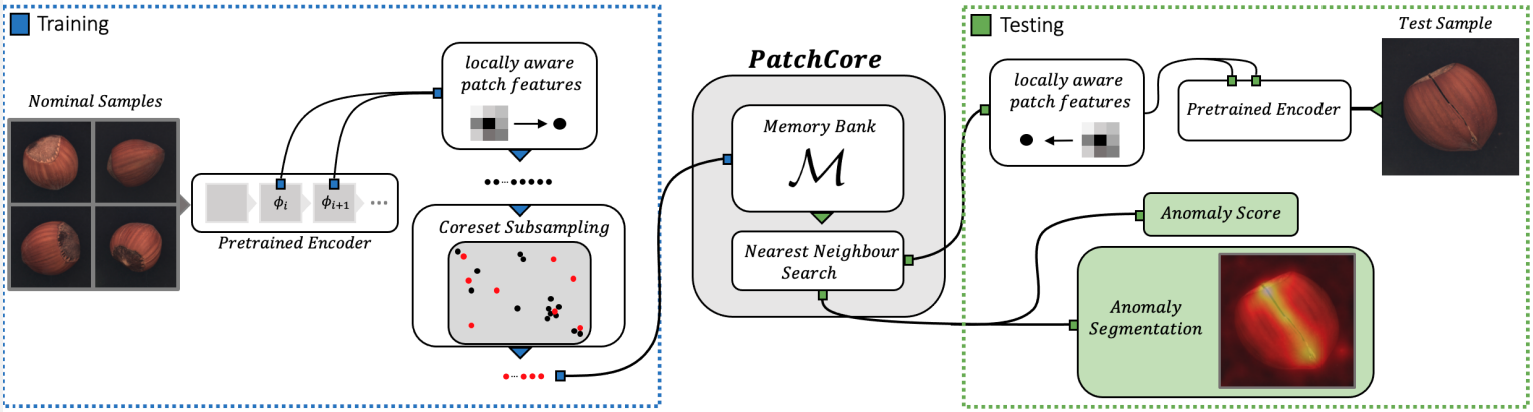
\includegraphics[width=0.95\textwidth]{bilder/patchcore.png}
    \caption{Skizze zur Funktionsweise von PatchCore. \cite{patchcore}} 
    \label{fig:PatchCore}
\end{figure}
\subsection{Erzeugen der Patch Features}\label{subsec:ErzeugenDerPatchFeatures}
Zunächst werden einige Notationen definiert, die im Folgenden verwendet werden und in analoger Form auch anderen Stellen in dieser Arbeit verwendet werden.\
So wird die Menge aller Trainingsbilder als $\mathcal{X}_{train}$ bezeichnet. Die Menge aller Testbilder als $\mathcal{X}_{test}$.\
Für den Trainingsdatensatz gilt im Sinne der Unüberwachtheit (TODO), dass es sich um ausschließlich nominale Samples handelt. Im Testdatensatz können sowohl nominale als auch anomale Samples enthalten sein.\
Bezeichnen wir die wahre Klassenzugehörigkeit eines Bildes $x$ als $y_{x}$, so kann diese entweder $0$ (nominal) oder $1$ (anomal) sein. Für den Trainingsdatensatz gilt dann:\
$\forall x \in \mathcal{X}_{train}: y_{x} = 0$ und für den Testdatensatz $\forall x \in \mathcal{X}_{test}: y_{x} \in \{0,1\}$.\\
Den bereits in \ref{sec:SPADE} und \ref{sec:PaDiM} angetroffenen \glqq Pretrained Encoder\grqq{} wird als $\phi$ bezeichnet.\
Es wird dabei, wie bereits gesehen, nicht der Ausgang dieses Netzwerkes benutzt, sondern die Feature Maps aus einer oder mehreren Schichten $j$ des Netzwerkes. \
Im Falle von ResNets, die auch in dieser Veröffentlichung hauptsächlich verwendet werden, ist $j\in \{1,2,3,4\}$.\ 
$j$ wird folgend auch als \glqq Hierarchielevel\grqq{} bezeichnet und spielt eine wichige Rolle.\
$\phi_{i,j} = \phi_{j}(x_{i})$ bezeichnet die Feature Map des Bildes $x_{i}\in \mathcal{X}$ aus den Hierarchieleveln $j$.\
Wie bereits in \ref{subsec:SPADEResults} diskutiert, ist eine sinnvolle Auswahl der Hierarchielevel eine wichtige Voraussetzung für gute Ergebnisse und wird in \ref{subsec:FeatureExtraktorWahlDesBackbonesPatchcore} genauer untersucht.\
Auch die Autoren von PatchCore weisen auf diese Problemstellung hin. Man könne, wie bei SPADE, die letzte Ebene in der Merkmalshierarchie des Netzes verwenden. \
Dies bringe aber die folgenden zwei Probleme mit sich. Erstens gehe dabei mehr lokalisierte nominale Informationen verloren. Das sei während der Trainingsphase kritisch,\
weil die Arten von Anomalien, die zum Testzeitpunkt auftreten, nicht im Voraus bekannt seien und die möglichst vollständige Erfassung des Normals notwendig sei.\
Zweitens seien die sehr tiefen und abstrakten Merkmale in den vortrainierten ImageNet-Netzwerken auf die Aufgabe der Klassifizierung natürlicher Bilder ausgerichtet,\
welche nur wenig direkte Überschneidungen mit der hier vorliegenden Aufgabe der industriellen Anomaliedetekion aufweise.\
Es wird deshalb vorgeschlagen, Merkmale aus den mittleren Hierarchielevels zu verwenden. Das entspricht bei ResNets $j=\{2,3\}$.\
Wie in \ref{fig:ResNetPyramid} zu erkennen, handelt es sich bei $\phi_{i,j}$ um einen dreidimensionalen Tensor: $\phi_{i,j}\in \mathbb{R}^{c^{*}\times h^{*}\times w^{*}}$\
mit $c^{*}$ als Tiefe der Feature Maps, $h^{*}$ als Höhe und $w^{*}$ als Breite. \
$\phi_{i,j}(h,w)\in\mathbb{R}^{c^{*}}$ bezeichnet dann den zur Position $h\in\{1,...,h^{*}\}$ und $w\in\{1,...,w^{*}\}$ gehörenden Vektor der Länge $c^{*}$.\
Unter der Annahmen, dass die Größe des Feldes im Originalbild $x_{i}$, das Einfluss auf ein $\phi_{i,j}(h,w)$ nimmt (\glqq Receptive Field\grqq{}), \
so groß ist, um einen ausreichenden räumlichen Kontext zu erfassen, eignet sich dieser Vektor als \glqq Patch Feature\grqq{} für eine gegenüber\
räumlichen Variationen robusten Anomaliedetektion.\\
Um diese wünschenswerte Annahme zu erfüllen, wird eine Aggregation der lokal umliegenden Regionen (\glqq local Neighborhood Aggregation\grqq{}) durchgeführt, das nachfolgend \
vorgestellt wird und die Größe des rezeptiven Feldes steuert.\\
Dafür wird die oben eingeführte Notation für $\phi_{i,j}(h,w)$ um eine ungerade Feldgröße (\glqq patchsize\grqq{}) $p$ erweitert, die die benachbarten Feauture Vektoren \
mit einbezieht. Zunächst wird diese Nachbarschaft wie folgt definiert:\
$$
\mathcal{N}_{p}^{(h,w)} = \left\{(a,b)| a \in \left[h-\left\lfloor \frac{p}{2}\right\rfloor,...,h+\left\lfloor \frac{p}{2} \right\rfloor\right], b \in \left[w-\left\lfloor \frac{p}{2}\right\rfloor,...,w+\left\lfloor \frac{p}{2}\right\rfloor\right]\right\}
$$ 
Damit ergeben sich schließlich ein \glqq Patch Feature\grqq{} zu\
$$
\phi_{i,j}\Big(\mathcal{N}_{p}^{(h,w)}\Big) = f_{agg}\Big(\{\phi_{i,j}(a,b)| (a,b) \in \mathcal{N}_{p}^{(h,w)}\}\Big),
$$
wobei $f_{agg}$ eine Aggregationsfunktion ist. Die Aggregationsfunktionsfunktion, die in der PatchCore Methode verwendet wird, ist ein adptives \glqq Average Pooling\grqq{}, \
in einer Dimension, die unabhängig von der Länge der Eingangsfeature, immer eine feste Länge $d$ ausgibt.\\
Da diese Operation für alle Paare von $(h,w)$ mit $h\in\{1,...,h^{*}\}$ und $w\in\{1,...,w^{*}\}$ durchgeführt wird, wird die Auflösung der Feature Map erhalten.
Für einen gesamten Feature Map Tensor ergibt sich dementsprechend:\
$$
\mathcal{P}_{p}\left(\phi_{i,j}\right) = \left\{\phi_{i,j}\Big(\mathcal{N}_{p}^{(h,w)}\Big)| h\in\{1,...,h^{*}\}, w\in\{1,...,w^{*}\}\right\}
$$
Wie bereits erwähnt, kann diese Operation für verschiedene Hierarchielevel geschehen. Weil die Auflösung der Feature Maps mit steigendem Hierarchielevel abnimmt,\
wird $\mathcal{P}_{p}\left(\phi_{i,j+1}\right)$ berechnet und anschließend auf die Auflösung von $\mathcal{P}_{p}\left(\phi_{i,j}\right)$ linear interpoliert.\
Jedes Element wird dann mit dem korrespondieren Element, also dem Element an der gleichen Stelle, aggregiert. Es ist also notwendig, dass für jedes $j$ die gleiche\
Featurelänge $d$ gewählt wird.\\
Würde auf eine Auswahl der Patch Feature, wie im folgenden Abschnitt erläutert, verzichtet, würde sich folgende Memory-Bank ergeben:
$$
\mathcal{M} = \bigcup_{x_i\in\mathcal{X}_{train}}\mathcal{P}_{s,p}\left(\phi_{i,j}\right)
$$
\subsection{Coreset Subsampling}\label{subsec:CoresetSubsampling}
Insbesondere, wenn $\mathcal{X}_{train}$ eine große Kardinalität hat, also viele Bilder enthält, wird die Memory-Bank $\mathcal{M}$ sehr groß. Wie bereits in \ref{sec:SPADE} festgestellt \
ist diese Kardinalität besonders laufzeitkritisch, weil die Nächste Nachbar Suche in der Memory-Bank mit einer Komplexität von $\mathcal{O}(n)$ berechnet wird. \ 
Wie bereits in \ref{sec:PaDiM} zu sehen, ist ein \glqq patchbasierter\grqq{} Vergleich zwischen allen Elementen in $\mathcal{M}$ und allen Elemnten in $\mathcal{P}_{s,p}\left(\phi_{i,j}\right)$ \
ein notwediger Schritt - nicht nur um die Anomaliekarte zu erstellen, die in dieser Arbeit ohnehin von keinem großen Interesse ist, sondern auch um eine robuste und \ 
präzise Instanzklassifizierung durchzuführen. Für die Laufzeitoptimierung ist es also wünschenswert, die Kardinalität der Memory-Bank zu reduzieren.\\
Auf der anderen Seite müssen die Elemente in $\mathcal{M}$ möglichst gut nominale Eigenschaften abbilden, um eine gute Anomaliedetektion zu ermöglichen.\
Wie in der Veröffentlichung gezeigt wird, (§4.4.2 - Importance of Coreset Subsampling) führt der naive Ansatz, zufällig Elemente aus $\mathcal{M}$ auszuwählen, \
nicht zu zufriedenstellenden Ergebnissen.\\
Das von PatchCore zugrundeliegenden Konzept setzt genau hier an. Es soll eine Teilmenge $\mathcal{S}\subset \mathcal{A}$ gefunden werden, bei der die Problemlösung \
über $\mathcal{A}$ am ehesten und vor allem schneller durch die über $\mathcal{S}$ berechnete Lösung approximiert werden kann. Dabei ist die Methode, \
die zu einer solchen Teilmenge führt, problemspezifisch. Im Falle von PatchCore wird eine Berechnung von Nächsten Nachbarn durchgeführt,\
weswegen gemäß \cite{sener2018active} eine \glqq MiniMax-Funktion\grqq{} sich anbietet, um eine annähernd ähnliche Abdeckung der $\mathcal{M}$ mit $\mathcal{M_{C}}$ zu erreichen.\
Dies kann wie folgt gelöst werden:\
$$
\mathcal{M_{C}^{*}} = \underset{\mathcal{M}_{C}\subset\mathcal{M}}{\arg\min}\underset{m\in\mathcal{M}}{\max}\underset{n\in\mathcal{M_{C}}}{\min}\left\|m-n\right\|_{2}
$$
Die exakte Berechnung von $\mathcal{M_{C}^{*}}$ ist NP-schwer, also nicht in polynomieller Zeit berechenbar.\
Es handelt sich zwar um einen Prozess, der nicht während der Inferenz durchgeführt werden muss, sondern einmalig während der Trainingsphase,\
aber es muss dennoch mit iterativen, approximierenden Verfahren gearbeitet werden.\\
Aus \cite{sener2018active} wird ein \glqq Greedy Algorithmus\grqq{} übernommen, der iterativ Elemente aus $\mathcal{M}$ auswählt, die die größte Distanz zu allen bereits ausgewählten Elementen haben.\
Um die Laufzeit des Subsamplings weiter zu reduzieren, wird das \glqq Johnson-Lindenstrauss Lemma\grqq{}\cite{johnsonlindenstrauss} verwendet, um die Dimensionalität der Elemente $m\in\mathcal{M}$\ 
durch zufällige lineare Projektion $\psi: \mathbb{R}^{d} \rightarrow \mathbb{R}^{d^{*}}$ mit $d^{*}<d$ zu reduzieren. Anschaulich kann dies durch eine Punktwolke erklärt werden, die aus zufälligen Blickwinkeln betrachtet wird, wodurch die 3-D-Struktur als 2-D Struktur\
angenähert wird.\
\subsection{Bestimmen des Anomaliegrades}\label{subsec:BestimmenDesAnomaliegradesPatchcore}
Wie bereits in der Einleitung zu diesem Katpitel erwähnt, ist die Grundlage der Bestimmung des Anomaliegrades die Distanz zu den Nächsten Nachbarn in der Memory-Bank.\ 
Das gilt sowohl für die Anomaliekarte bzw. die Segmentierung, als auch für die Instanzklassifizierung. \
Zunächst muss während der Inferenz aus einem Testbild $x_{i}\in\mathcal{X}_{test}$ die Patch Features extrahiert werden. Dies geschieht auf die gleiche Weise, wie in der Trainingsphase:\
$$
\mathcal{P}\left(x_{i}\right)= \mathcal{P}_{p}\left(\phi_{j}\left(x_{i}\right)\right)
$$
Diese Menge $\mathcal{P}\left(x_{i}\right)$ enthält nun die Patch Features $m^{test}$ des Testbildes $x_{i}$. Nun gilt es zu jedem Patch Feature in $\mathcal{P}\left(x_{i}\right)$ \
den Nächsten Nachbarn in der Memory Bank $\mathcal{M}$ zu finden:\
$$
m^{*} = \underset{m\in\mathcal{M}}{\arg\min}\left\|m-m^{test}\right\|_{2}, \forall m^{test}\in\mathcal{P}\left(x_{i}\right)
$$
Es gilt zu beachten, dass jedes $m^{test}$ zu einer Position $(h,w)$ im Bild $x_{i}$ gehört.\
So kann eine räumlich aufgelöste Anomaliekarte $M$ erzeugt werden, die die Distanz zu den Nächsten Nachbarn in der Memory-Bank enthält:
$$
% M = \left\{m^{*}(h,w)| m^{*} = \underset{m\in\mathcal{M}}{\arg\min}\left\|m-m^{test}\right\|_{2}, \forall m^{test}\in\mathcal{P}\left(x_{i}\right)\right\}
M = \Big(\left\|m^{*}_{h,w}-m^{test}_{h,w}\right\|_{2}\Big)_{h,w},\forall \left(h,w\right)\in\{1,...,h^{*}\}\times\{1,...,w^{*}\} % m^{test}_{h,w}\in\mathcal{P}\left(x_{i}\right)
$$
Diese Anomaliekarte $M$ kann schließlich mittels bilinearer Interpolation und einer anschließenden Glättung auf die Auflösung des Originalbildes $x_{i}$ gebracht werden, wodurch eine \
pixelweise Klassifikationskarte möglich wird. Weil dies in dieser Arbeit nicht von Interesse ist, wird darauf nicht weiter eingegangen.\\
Die Instanzklassifizierung könnte nun analog zu PaDiM (\ref{subsec:PaDiMFunktionsweise}) durch Maximalwerbildung durchgeführt werden.\
Die Autoren von PatchCore gehen ähnlich vor, fügen jedoch noch einen Gewichtungsschritt hinzu.\
Zunächst wird ganz analog vorgegangen und die maximale Distanz zu den Nächsten Nachbarn herangezogen, was nichts anderes als der Maximalwert der Anomaliekarte $M$ ist.\
$$
m^{test,*}, m^{\star}=\underset{m^{test}\in\mathcal{P}(x_{i})}{\arg\max}\underset{m\in\mathcal{M}}{\arg\min}\left\|m-m^{test}\right\|_{2}
$$
$$
s^{*}=\left\|m^{test,*}-m^{\star}\right\|_{2}=\max\{M\}
$$
Die Gewichtung schließt die nächsten $b$ Patch Features in $M$ zu $m^{\star}$ mit ein. Diese Menge notieren wir als $\mathcal{T}_{b}\left(m^{\star}\right)$.\
Der Gedanke hinter dieser Gewichtung ist, den Anomaliegrad $s$ dann zu erhöhen, wenn die Feature Patches in $\mathcal{T}_{b}\left(m^{\star}\right)$ selbst \
weit entfernt vom Anomaliekandidaten Patch Feature $m^{\star}$ sind und es sich somit ohnehin um seltene nominale Patch Features handelt. \
Der finale, für die Instanzklassifiziergung entscheidende Anomaliegrad $s$ ergibt sich dann zu:\
$$
s = \left(1-\frac{e^{\left\|m^{\star}-m^{test,*}\right\|_{2}}}{\sum\nolimits_{m\in\mathcal{T}_{b}\left(m^{\star}\right)}e^{\left\|m-m^{test,*}\right\|_{2}}}\right) \cdot s^{*}
$$
Durch diese Gewichtung wird die Instanzklassifizierung robuster und erhöht die Instanzklassifiziergungsgenauigkeit.\
\section{Ergebnisse und Diskussion der Originalmethode}\label{sec:ErgebnisseUndDiskussionDerOriginalmethode}
\textcolor{green}{\textit{Abgeschlossen: 01.11. v1}}\\
In diesem Abschnitt werden die Ergebnisse der Originalmethode PatchCore vorgestellt und diskutiert.\
Dies soll vor allem im Hinblick auf die Eignung für eine Implementierung auf einem ressourcenbeschränkten Gerät, nämlich einem RaspberryPi 4B (\ref{sec:RaspberryPi4B}) geschehen.\
Es wird sich dabei auf den hier verwendeten Datensatz MVTecAD (\ref{sec:DatensatzMVTecAD}) bezogen. Weitere Datensätze, die in der Veröffentlichung verwendet wurden, \
werden mit dem Verweis auf die Veröffentlichung nicht weiter betrachtet. Die zur Evaluation herangezogene Metrik ist AUROC (\ref{sec:AUROC}).\\
Wie bereits in der Einleitung erwähnt, ist die Methode PatchCore grundsätzlich in der Lage, sehr hohe Instanzklassifiziergungsgenauigkeiten zu erreichen, die auch zwei Jahre nach \
Veröffentlichung noch zu den besten gehören. Erreicht wird dies teilweise durch ein Ensemble von verschiendenen Feature Extraktoren bzw. Backbones und höhere Auflösungen.\
So wird ein \glqq DenseNet 201\grqq{}\cite{densenet}, ein \glqq ResNext 101\grqq{}\cite{resnext} und ein bereits bekanntes Wide ResNet mit 101 Schichten \cite{wideresnet} verwendet. \
Steht eine GPU zur Verfügung, welche, wie in \ref{tab:model-runtimes} zu sehen, die Laufzeit von CNNs deutlich reduziert, können selbst mit einer solchen Konfiguration, bestehend aus \
vielen Backbones, einigermaßen schnelle Inferenzzeiten erreicht werden.\
Da die Zielsetzung dieser Arbeit jedoch die Implementierung auf einem RaspberryPi 4B ist und bereits gezeigt wurde, dass das Ausführen von CNNs auf einem solchen Gerät \
äußerst laufzeitkritisch ist, ist eine solche Konfiguration im Kontext dieser Arbeit nicht sinnvoll.\
Beschränken wir uns auf Konfigurationen, mit nur einem Backbone und auf die Auflösung von $256\times 256$ Pixeln, so erreicht PatchCore mit einem Wide ResNet-50 Backbone eine \
Instanzklassifiziergungsgenauigkeit (AUROC) von \num{99,1} mit einer Reduktion der Memory Bank auf \num{25}\%. Wird die Größe der Memory Bank auf \num{1}\% reduziert, \
verschlechtert sich der AUROC nur leicht auf \num{99,0}\%. Wie im Laufe dieses Kapitels noch zu sehen sein wird, ist die Reduzierung der Kardinalität der Memory Bank \
ein wichtiger Schritt, um die Laufzeit zu reduzieren. Die hier angewandte Methode des Coreset Subsamplings ist also ein wichtiger Bestandteil und eine Errungenschaft \ 
der Methode PatchCore.\\
Neben dem Erzeugen der Patch Feature ist die Nächste Nachbar Suche in der Memory Bank besonder laufzeitkritisch. In der Veröffentlichung lediglich eine kleine Randnotiz im Anhang, \
ist diese Suche mit \glqq FAISS\grqq{} implementiert. FAISS ist eine Bibliothek, entwickelt von Facebook's AI Research Department, die die Nächste Nachbar Suche \ 
enorm beschleunigt und im Laufe dieses Kapitels (Abbildung \ref{fig:patchcorecdist}) nochmal genauer erläuert und analysiert wird.\\
Insgesamt ist die Methode PatchCore zwar in ihrer Originalform eine ausgezeichnete Basis, aber für die Implementierung auf einem RaspberryPi 4B nur eingeschränkt geeignet.\
Es werden im Folgenden zahlreiche Adaptionen vorgestellt und evaluiert, die das Ziel haben, die Laufzeit zu reduzieren und dabei möglichst viel der Genauigkeit zu erhalten.\ 
\section{Testaufbau}\label{sec:Testaufbau}
In diesem Abschnitt wird die Testumgebung vorgestellt, die für die Evaluation der PatchCore Methode verwendet wurde.\ 
Dabei sind viele der hier aufgeführten Vorgehensweisen auf \ref{ch:EfficientAD} und \ref{ch:SimpleNet} übertragbar.\
\subsection*{Hardware}\label{subsec:Hardware}
Es stehen grundsätzlich zwei Testumgebungen zur Verfügung. Das Ziel ist es zwar, die Implementierung auf einem RaspberryPi 4B zu ermöglichen,\
auf dem Weg dorthin, ist eine potentere Hardware aber notwendig. \\
Die Entwicklungsgeschwindigkeit hängt zum einen auch von der Laufzeit der Trainingsphase ab, die auf einem RaspberryPi 4B sehr lange dauert.\
Außerdem sind Ergebnisse, die auf der Desktop-Hardware erzeugt wurden, im Falle der Genauigkeit ganzheitlich übertragbar, nehmen, aber nur einen Bruchteil der Zeit in Anspruch.\
So spielt die Hardware, auf der eine identische Methode ausgeführt wird, für die Instanzklassifiziergung keine Rolle.\
Sind also lediglich die Instanzklassifiziergungsgenauigkeiten in einem Abschnitt von Relevanz, weil keine oder bekannte Unterschiede in der Laufzeit bestehen, kann auch auf eine \
GPU zurückgegriffen werden.\\
Laufzeitmessungen werden über weite Teile dieser Arbeit auf der Desktop-Hardware durchgeführt. Zwar sind nicht nur die reine Rechenleistung zwischen den Prozessoren der beiden Geräten \
unterschiedlich, auch die CPU-Architektur (ARM vs. x86) spielt eine Rolle. Jedoch sind die Ergebnisse qualitativ übertragbar. Aufgrund der Vielzahl an Adaptionen, die im Laufe dieser Arbeit \
getestet werden, wurde sich dazu entschlossen, die Laufzeitmessungen nur dann auf dem RaspberryPi 4B durchzuführen, wenn entweder große relative Abweichungen zu den Messungen auf der Desktop-Hardware \
zu erwarten sind oder es sich um eine finale Konfiguration handelt.\\
Im Folgenden werden einige relevante Informationen zum Desktop-System aufgeführt.\\
\begin{itemize}
    \item CPU: AMD Ryzen 5 5600X (6 Kerne, 12 Threads, @ 3,7 GHz)
    \item RAM: 32 GB DDR4 @ 3200 MHz
    \item GPU: Nvidia GeForce RTX 3060Ti (8 GB GDDR6)
    \item OS: Ubuntu 23.10 (Linux, Kernel 6.2.0-generic)
\end{itemize}  
Detailierte Information zur Hardware des RaspberryPi finden sich in \ref{sec:RaspberryPi4B}.\\
\subsection{Software}\label{subsec:Software}
Wie in der Forschung weit verbreitet und auch in allen Veröffentlichungen, die in dieser Arbeit verwendet werden, wird die Programmiersprache \textbf{Python} verwendet.\
Es kommt dabei die Version \textit{3.10} zum Einsatz.\\
Ebenfalls der Konvention in der Forschung entsprechend, wird das \textbf{PyTorch} Framework in der Version \textit{2.0.1} verwendet.\
PyTorch ist ein Open-Source-Framework für maschinelles Lernen, das von Facebooks AI Research Lab (FAIR) entwickelt wurde. Es hat aufgrund seiner Flexibilität, \ 
seines dynamischen Berechnungsgraphen und seiner Benutzerfreundlichkeit in der Community für maschinelles Lernen und Deep Learning große Beliebtheit erlangt. \ 
PyTorch bietet eine Python-basierte Schnittstelle für die Entwicklung neuronaler Netze und anderer Modelle für maschinelles Lernen. \
kann mit PyTorch effizient abgebildet werden.\cite{pytorch}\\
Die Nächste Nachbar Suche wird mit der Bibliothek \textbf{FAISS} durchgeführt. FAISS ist eine Bibliothek, die von Facebooks AI Research Lab (FAIR) entwickelt wurde. \
Wie bereits im vorherigen Abschnitt erwähnt, wird die Nächste Nachbar Suche jedoch in den meisten Fällen mit der Bibliothek \textbf{FAISS} durchgeführt. \ 
FAISS (Facebook AI Similarity Search) ist eine leistungsstarke Bibliothek, die ebenfalls vom KI-Forschungsteam von Facebook (FAIR) für die effiziente und \ 
skalierbare Ähnlichkeitssuche und die Suche nach dem nächsten Nachbarn in großen Datensätzen entwickelt wurde. \
FAISS wurde insbesondere für die Verarbeitung hochdimensionaler Daten entwickelt und eignet sich daher besonders \ 
gut für Aufgaben, die Merkmalsvektoren beinhalten, wie z. B. Einbettungen aus Deep-Learning-Modellen. Es nutzt Techniken wie Indexstrukturen, Quantisierung \ 
und GPU-Beschleunigung, um Suchvorgänge erheblich zu beschleunigen.\cite{faiss} \\
Daneben werden bekannte Bibliotheken wie \textbf{numpy} oder \textbf{scikit-learn} verwendet. Zur besseren Organisation des Codes wird ein modularer Aufbau verwendet, \
der durch das Framework \textbf{pytorch lightning} ermöglicht wird.\\
\subsubsection*{Laufzeit- und AUROC-Messungen}\label{subsubsec:LaufzeitUndAUROCMessungen}
Die Laufzeitmessungen werden mit dem Python-Modul \textbf{time} bzw. der Methode \textbf{perf\_counter()} durchgeführt.\
Zunächst wird immer nur die Laufzeit für ein einzelnes Bild betrachtet. Erst im Anschluss wird mit dem Durchsatz (\glqq Throughput\grqq{}) die Laufzeit von einem Ensemble (Batch)
an Bildern betrachtet (TODO --> Ref). \\
Ein einzelnes Bild durchläuft, während einer Laufzeitmessung $3$ mal einen sogenannten \glqq Warm-Up\grqq{} Prozess, der im Wesentlichen dazu dient, \
mögliche Overheads in Form von Initialisierungsprozessen, die im Hintergrund ablaufen, auszuschließe und zusätzliche, die Hardware in einen authentischen thermischen Zustand zu bringen.\
Keiner dieser Prozesse geht in die Laufzeitmessung direkt ein. Diese folgt für jedes Bild einzeln, indem die Inferenz $5$ mal durchgeführt wird und die Laufzeiten gemittelt werden. \
Es werden hierbei $5$ Zeitpunkte innerhalb des Prozesses mit \textit{perf\_counter()} festgestellt. Diese sind:\
\begin{itemize}
    \item \textbf{Start}: Der Zeitpunkt, an dem die Inferenz beginnt.
    \item \textbf{Ende: Feature Extraktion}: Der Zeitpunkt, an dem die Feature Extraktion durch den Backbone abgeschlossen ist (\ref{subsec:ErzeugenDerPatchFeatures}).
    \item \textbf{Ende: Einbettungsprozess}: Der Zeitpunkt, an dem die Patch Feature vorliegen (\ref{subsec:ErzeugenDerPatchFeatures}).
    \item \textbf{Ende: Nächste Nachbar Suche}: Der Zeitpunkt, an dem die Nächse Nachbar Suche abgeschlossen ist.
    \item \textbf{Ende: Anomalieprozess}: Der Zeitpunkt, an dem der Anomaliegrad berechnet wurde und der damit Prozess abgeschlossen ist (\ref{subsec:BestimmenDesAnomaliegradesPatchcore}). 
\end{itemize}
Aus den Differenzen dieser Zeitstempel lassen sich dann präzise die Laufzeiten für die einzelnen Prozesse und den Gesamtprozess bestimmen. Da es jedoch zu Schwankungen in der Laufzeit \
kommt, ist eine Mittelwertbildung notwendig. Dies geschieht in zweifacher Hinsicht. Zunächst wird für jedes Bild über die $5$ Durchläufe gemittelt. \
Das wird für jedes Bild wiederholt, sodass für jedes Bild eine Laufzeit vorliegt. Aus diesen Laufzeiten wird dann ebenfalls der Mittelwert gebildet, der als eigentlicher Messwert für eine \
Konfiguration dient.\\
Anzumerken ist, dass in dieser Arbeit, wie bereits in \ref{sec:AUROC} erläutert, auf eine Segmentierung verzichtet wird. Dementsprechend wird dieser Prozess, soweit nicht für die \
Instanzklassifiziergung notwendig, übersprungen und insbesondere nicht laufzeittechnisch erfasst.\\
Ebenfalls wird der Initialisierungsprozess bzw. die Trainingsphase nur in exemplarischen Fällen betrachtet. Der Initialisierungsprozess ist einmalig und kann auch somit auch auf potenter Hardware \
durchgeführt werden. In einer produktiven Umgebung ist dieser Trainingsprozess ohnehin nicht relevant, weil bereits abgeschlossen.\\
Wie in (TODO --> ref) zu sehen, hängt die Laufzeit, genauer gesagt, die NN-Suche, stark von der Kardinalität von der Memory Bank $\mathcal{M}$ ab. In der Literatur allgemein üblich ist, \
dass ein relatives Subsampling stattfindet. Wie wir \ref{tab:mvtecad_overview} entnehmen können, hat jede Kategorie unterschiedlich viele Bilder im Trainingsdatensatz und teilweise verschiedene\
Auflösungen, wodurch sich eine unterschiedliche absolute Anzahl an Patch Featuren ergeben. Um die Laufzeitmessungen vergleichbar zu machen, wird die Kardinalität der Memory Bank \
in den meisten Fällen auf $\num{1000}$ gesetzt, wenn nicht anders angegeben. Dies dient vor allem dazu, die Laufzeitmessungen für alle Klassen gleichermaßen geltend zu machen.\
In diesem Sinne werden auch die Auflösungen der Bilder auf $256\times 256$ Pixel gesetzt, was dem Vorgehen der meisten Veröffentlichungen in diesem Bereich entspricht. Der Skalierungsprozess wird \
dabei nicht als Teil der Laufzeit betrachtet. \\
Dieser ermöglicht, dass die Laufzeitmessung für eine Konfiguration für eine Klasse ausreichend ist. Dies reduziert den Zeitaufwand für eine Messung einer Konfiguration über alle Klassen deutlich,\
weil zum einen auf die Wiederholungen verzichtet werden kann, andererseits für die verbleibende Bestimmung der AUROC auch eine deutlich schneller arbeitende GPU verwendet werden kann.\\
Wie bereits in \ref{sec:AUROC} ausgeführt, ist die AUROC eine ideale Metrik um die Güte eines Anomaliedetektors zu bewerten.\
Hierzu werden zunächst für alle Bilder im Testdatensatz die Anomaliegrade berechnet. Auf Grundlage dieser Werte, wird dann die AUROC berechnet.\
Wie in \ref{subsec:CoresetSubsampling} ausgeführt, wird bei der Berechnung der Elemente, die in die Memory-Bank übernommen werden, ein Algorithmus verwendet, der 
randomisiert arbeitet. Um diesen zufälligen Einfluss zu minimieren, werden aus den identischen Patch Featuren $5$ Memory Banks $\mathcal{M}$ erzeugt, deren AUROC ebenfalls gemittelt wird,\
um einen möglichst konsistenten Schätzer zu erhalten. Das geschieht für alle Klassen aus MVTecAD (\ref{sec:DatensatzMVTecAD}) und der Klasse des einigen Datensatzes (Granulat, \ref{sec:EigenerDatensatz}).\
Während für den eigenen Datensatz der AUROC explizit angegeben wird, wird für die Klassen aus MVTecAD nur der Mittelwert über alle Klassen angegeben. Die einzelnen Ergebnisse sind aber archiviert und können \
beim Autor erfragt werden.\\
Die meisten der hier zu sehenden Plots wurden mit \textbf{tikz} und \textbf{matplotlib} direkt auf Grundlage der Messergebnisse erzeugt. Die Annotationen sind sinnvoll gerundet, um eine bessere \
Lesbarkeit zu ermöglichen. \\
Die Grundlage der Implementierung der Methode PatchCore liefert dabei die offizielle Implementierung \cite{patchcore} und eine inoffizielle Implementierung \cite{unofficialimplementation}. Diese wurden jedoch jeweils derart modifiziert, dass
nur noch wenige Elemente der ursprünglichen Implementierung übrig geblieben sind. Der gesamte Code mit dem die folgenden Ergebnisse und Messungen erzeugt wurden, ist abrufbar.\
\section{Adaptionen und Messergebnisse}\label{sec:Adaptionen}
Der hier beginnende Abschnitt ist der umfangreichste dieser Arbeit. Er besteht als vielen Adaptionen, die im Laufe der Arbeit durchgeführt wurden, um die Laufzeit zu reduzieren.\
Jeder Unterabschnitt beschäftigt sich damit mit einer Adaption oder einer Kombination von Adaptionen. \ 
Zunächst wird dabei, die Idee hinter der Adaption erläutert. Messergebnisse werden dann präsentiert und diskutiert. Schließlich findet eine Einordnung und Bewertung statt.\
\subsection{Originalmethode}
Zunächst wird die Originalmethode ohne Adaption betrachtet. Es wird also die Methode PatchCore mit einem Wide ResNet-50 Backbone und einer Auflösung von $256\times 256$ Pixeln verwendet.\
Die Laufzeitmessungen wurden mit der CPU des Desktop-PCs durchgeführt.\\
In \ref{fig:patchcoreoriginal} ist die Laufzeit für die einzelnen Prozesse und den Gesamtprozess zu sehen, sowie die erreichte AUROC Klassifizierungsgenauigkeit.\
Es lässt sich erkennen, dass die Angaben aus dem Paper sich verifizieren lassen. Es kann daraus abgeleitet werden, dass die im Rahmen dieser Arbeit erarbeitete Implementierung \
korrekt ist.\\
Eine schon besprochene Bemerkung kann ebenfalls abgelesen werden. Die von PatchCore verwendete Subsampling-Methode ist in der Lage, die Kardinalität der Memory Bank $\mathcal{M}$ \
deutlich zu reduzieren, ohne die AUROC Klassifizierungsgenauigkeit zu stark zu beeinflussen. Eindeutig ist auch zu erkennen, dass diese Reduktion der Kardinalität \
ein wesentlicher Bestandteil ist, möchte man eine möglichst geringe Laufzeit erreichen. Trotz Verwendung der State-of-the-Art Methoden, die von FAISS bereitgestellt werden, \
ist die Nächste Nachbar Suche der laufzeitkritischste Prozess, wenn ein Subsampling $>10\%$ verwendet werden soll.\\
Am Granulatdatensatz lässt sich sogar feststellen, dass zumindest in einzelnen Fällen, ein Subsampling der Instanzklassifiziergungsgenauigkeit sogar zuträglich sein kann.\
Wie bereits ausgeführt, wird im Rahmen dieser Arbeit in den meisten Fällen kein relatives Subsampling durchgeführt, sondern eine absolute Kardinalität von $\num{1000}$ verwendet.\
Für manche Klassen mit wenigen Trainingsbeispielen und geringerer Auflösung bedeutet das, es werden mehr Patch Feature in der Memory Bank sein, als bei einem relativen Subsampling mit $1\%$.\
In den meisten Fällen läge die relative Subsamplingrate, die eine Kardinalität von $\num{1000}$ erzeugt, bei $<1\%$. Berechnet man den Mittelwert über alle Klassen, so ergibt sich eine \
durchschnittliche relative Subsamplingrate von $\approx \num{0,6}\%$. Die erzeugten Ergebnisse entsprechen somit den Erwartungen und den Ergebnissen aus der Veröffentlichung.\\
\begin{figure}[h]
    \centering
    % This file was created with tikzplotlib v0.10.1.
\begin{tikzpicture}  
  \newcommand{\widthplot}{0.8}
  \newcommand{\heightplot}{0.6}
  \newcommand{\anchorx}{1.1}


\definecolor{crimson}{RGB}{220,20,60}
\definecolor{darkgoldenrod}{RGB}{184,134,11}
\definecolor{darkgray176}{RGB}{176,176,176}
\definecolor{gray}{RGB}{128,128,128}
\definecolor{lightgray204}{RGB}{204,204,204}
\definecolor{purple}{RGB}{128,0,128}
\definecolor{slateblue}{RGB}{106,90,205}

\begin{axis}[  
  width=\widthplot\textwidth,
  height=\heightplot\textwidth,
legend cell align={left},
legend style={
  fill opacity=0.8,
  draw opacity=1,
  text opacity=1,
  at={(\anchorx,0.00)},
  anchor=south west,
  text width=2.25cm
},
tick align=outside,
tick pos=left,
x grid style={darkgray176},
xmin=-0.638, xmax=4.598,
xtick style={color=black},
xtick={0,1,2,3,4},
xticklabels={
 {\num{0,1}\%},{\#1000\\ MW $\approx \num{0,6}$\%},{1\%},{10\%},{100\%}
 },
xticklabel style={align=center},y grid style={darkgray176},
ylabel={(Lauf-) Zeit [ms]},
ymin=0, ymax=1200,
ytick style={color=black},
ytick={0,200,400,600,800,1000,1200},
yticklabels={{0,0},{200,0},{400,0},{600,0},{800,0},{1000,0},{1200,0}}
]
\draw[draw=none,fill=crimson] (axis cs:-0.4,0) rectangle (axis cs:0,49.2657432556152);
\addlegendimage{ybar,ybar legend,draw=none,fill=crimson}
\addlegendentry{Extraktion}

\draw[draw=none,fill=crimson] (axis cs:0.6,0) rectangle (axis cs:1,48.759349822998);
\draw[draw=none,fill=crimson] (axis cs:1.6,0) rectangle (axis cs:2,50.5632286071777);
\draw[draw=none,fill=crimson] (axis cs:2.6,0) rectangle (axis cs:3,50.2985725402832);
\draw[draw=none,fill=crimson] (axis cs:3.6,0) rectangle (axis cs:4,47.9584121704102);
\draw[draw=none,fill=purple] (axis cs:-0.4,49.2657432556152) rectangle (axis cs:0,87.7047691345215);
\addlegendimage{ybar,ybar legend,draw=none,fill=purple}
\addlegendentry{Einbettung}

\draw[draw=none,fill=purple] (axis cs:0.6,48.759349822998) rectangle (axis cs:1,79.8165168762207);
\draw[draw=none,fill=purple] (axis cs:1.6,50.5632286071777) rectangle (axis cs:2,79.4835166931152);
\draw[draw=none,fill=purple] (axis cs:2.6,50.2985725402832) rectangle (axis cs:3,89.3854598999023);
\draw[draw=none,fill=purple] (axis cs:3.6,47.9584121704102) rectangle (axis cs:4,87.7231483459473);
\draw[draw=none,fill=slateblue] (axis cs:-0.4,87.7047691345215) rectangle (axis cs:0,88.901162147522);
\addlegendimage{ybar,ybar legend,draw=none,fill=slateblue}
\addlegendentry{NN-Suche}

\draw[draw=none,fill=slateblue] (axis cs:0.6,79.8165168762207) rectangle (axis cs:1,84.9496912956238);
\draw[draw=none,fill=slateblue] (axis cs:1.6,79.4835166931152) rectangle (axis cs:2,88.9350080490112);
\draw[draw=none,fill=slateblue] (axis cs:2.6,89.3854598999023) rectangle (axis cs:3,181.543525695801);
\draw[draw=none,fill=slateblue] (axis cs:3.6,87.7231483459473) rectangle (axis cs:4,954.664310455322);
\draw[draw=none,fill=darkgoldenrod] (axis cs:-0.4,88.901162147522) rectangle (axis cs:0,88.9232767689973);
\addlegendimage{ybar,ybar legend,draw=none,fill=darkgoldenrod}
\addlegendentry{Anomaliegrad}

\draw[draw=none,fill=darkgoldenrod] (axis cs:0.6,84.9496912956238) rectangle (axis cs:1,84.9781920406967);
\draw[draw=none,fill=darkgoldenrod] (axis cs:1.6,88.9350080490112) rectangle (axis cs:2,88.965379146859);
\draw[draw=none,fill=darkgoldenrod] (axis cs:2.6,181.543525695801) rectangle (axis cs:3,181.573772054166);
\draw[draw=none,fill=darkgoldenrod] (axis cs:3.6,954.664310455322) rectangle (axis cs:4,954.758699148893);
\draw (axis cs:-0.2,49.2657432556152) ++(0pt,-2pt) node[
  scale=1.0,
  anchor=south,
  text=black,
  rotate=0.0
]{49,27};
\draw (axis cs:0.8,48.759349822998) ++(0pt,-2pt) node[
  scale=1.0,
  anchor=south,
  text=black,
  rotate=0.0
]{48,76};
\draw (axis cs:1.8,50.5632286071777) ++(0pt,-2pt) node[
  scale=1.0,
  anchor=south,
  text=black,
  rotate=0.0
]{50,56};
\draw (axis cs:2.8,50.2985725402832) ++(0pt,-2pt) node[
  scale=1.0,
  anchor=south,
  text=black,
  rotate=0.0
]{50,30};
\draw (axis cs:3.8,47.9584121704102) ++(0pt,-2pt) node[
  scale=1.0,
  anchor=south,
  text=black,
  rotate=0.0
]{47,96};
\draw (axis cs:-0.2,88.9232767689973) ++(0pt,-2pt) node[
  scale=1.0,
  anchor=south,
  text=black,
  rotate=0.0
]{88,92};
\draw (axis cs:0.8,84.9781920406967) ++(0pt,-2pt) node[
  scale=1.0,
  anchor=south,
  text=black,
  rotate=0.0
]{84,98};
\draw (axis cs:1.8,88.965379146859) ++(0pt,-2pt) node[
  scale=1.0,
  anchor=south,
  text=black,
  rotate=0.0
]{88,97};
\draw (axis cs:2.8,181.573772054166) ++(0pt,-2pt) node[
  scale=1.0,
  anchor=south,
  text=black,
  rotate=0.0
]{181,57};
\draw (axis cs:3.8,954.758699148893) ++(0pt,-2pt) node[
  scale=1.0,
  anchor=south,
  text=black,
  rotate=0.0
]{954,76};
\end{axis}

\begin{axis}[  
  width=\widthplot\textwidth,
  height=\heightplot\textwidth,
axis y line=right,
legend cell align={left},
legend style={
  fill opacity=0.8,
  draw opacity=1,
  text opacity=1,
  at={(\anchorx,1.00)},
  anchor=north west,
  text width=2.25cm},
tick align=outside,
x grid style={darkgray176},
xmin=-0.638, xmax=4.598,
xtick pos=left,
xtick style={color=black},
xtick={0,1,2,3,4},
xticklabels={},
y grid style={darkgray176},
ylabel={AUROC [\%]},
ymin=50, ymax=105,
ytick pos=right,
ytick style={color=black},
yticklabel style={anchor=west}
]
\draw[draw=none,fill=black] (axis cs:0.04,0) rectangle (axis cs:0.16,92.2260522842407);
\addlegendimage{ybar,ybar legend,draw=none,fill=black}
\addlegendentry{Granulat}

\draw[draw=none,fill=black] (axis cs:1.04,0) rectangle (axis cs:1.16,93.2260513305664);
\draw[draw=none,fill=black] (axis cs:2.04,0) rectangle (axis cs:2.16,94.296932220459);
\draw[draw=none,fill=black] (axis cs:3.04,0) rectangle (axis cs:3.16,93.5172438621521);
\draw[draw=none,fill=black] (axis cs:4.04,0) rectangle (axis cs:4.16,93.1800782680511);
\draw[draw=none,fill=gray] (axis cs:0.24,0) rectangle (axis cs:0.36,96.1345851421356);
\addlegendimage{ybar,ybar legend,draw=none,fill=gray}
\addlegendentry{MVTecAD}

\draw[draw=none,fill=gray] (axis cs:1.24,0) rectangle (axis cs:1.36,98.6910760402679);
\draw[draw=none,fill=gray] (axis cs:2.24,0) rectangle (axis cs:2.36,98.9949345588684);
\draw[draw=none,fill=gray] (axis cs:3.24,0) rectangle (axis cs:3.36,99.031263589859);
\draw[draw=none,fill=gray] (axis cs:4.24,0) rectangle (axis cs:4.36,99.0479826927185);
\draw (axis cs:0.1,92.2260522842407) ++(0pt,-2pt) node[
  scale=1.0,
  anchor=south,
  text=black,
  rotate=0.0
]{92,2};
\draw (axis cs:1.1,93.2260513305664) ++(0pt,-2pt) node[
  scale=1.0,
  anchor=south,
  text=black,
  rotate=0.0
]{93,2};
\draw (axis cs:2.1,94.296932220459) ++(0pt,-2pt) node[
  scale=1.0,
  anchor=south,
  text=black,
  rotate=0.0
]{94,3};
\draw (axis cs:3.1,93.5172438621521) ++(0pt,-2pt) node[
  scale=1.0,
  anchor=south,
  text=black,
  rotate=0.0
]{93,5};
\draw (axis cs:4.1,93.1800782680511) ++(0pt,-2pt) node[
  scale=1.0,
  anchor=south,
  text=black,
  rotate=0.0
]{93,2};
\draw (axis cs:0.3,96.1345851421356) ++(0pt,-2pt) node[
  scale=1.0,
  anchor=south,
  text=black,
  rotate=0.0
]{96,1};
\draw (axis cs:1.3,98.6910760402679) ++(0pt,-2pt) node[
  scale=1.0,
  anchor=south,
  text=black,
  rotate=0.0
]{98,7};
\draw (axis cs:2.3,98.9949345588684) ++(0pt,-2pt) node[
  scale=1.0,
  anchor=south,
  text=black,
  rotate=0.0
]{99,0};
\draw (axis cs:3.3,99.031263589859) ++(0pt,-2pt) node[
  scale=1.0,
  anchor=south,
  text=black,
  rotate=0.0
]{99,0};
\draw (axis cs:4.3,99.0479826927185) ++(0pt,-2pt) node[
  scale=1.0,
  anchor=south,
  text=black,
  rotate=0.0
]{99,0};

\draw[black, dashed] (axis cs:-1,100) -- (axis cs:5,100);\end{axis}

\end{tikzpicture}

    \caption{PatchCore: Originalmethode mit unterschiedlicher Anzahl an Patch Featuren in Memory Bank.}
    \label{fig:patchcoreoriginal}
\end{figure}
Der in der Originalmethode verwendete Einbettungsprozess, der in \ref{subsec:ErzeugenDerPatchFeatures} beschrieben ist, bietet einen Parameter $d$, der die Länge der Patch Features bestimmt.\
In der \ref{fig:patchcoreoriginal} wurde keine Dimensionsreduktion durchgeführt, indem $d$ der Länge der aus Layer3 ($j=3$) extrahierten Feature entspricht, nämlich $1024$.\
Mithilfe eines kleineren Parameters $d$ kann die Laufzeit weiter reduziert werden. In \ref{fig:patchcoreoriginal} ist die Laufzeit für unterschiedliche Werte von $d$ und zwei verschiedenen \ 
Methoden zur Bestimmung der Nächsten Nachbarn und den korrespondierenden Distanzen zu sehen. Diese Abbildung inkludiert bei (1) und (4) Einbettungsmethoden, die nicht in der Originalmethode \ 
vorgeschlagen worden sind und in Abschnitt (TODO --> ref) erläutert werden.\
An dieser Stelle ist wichtig, dass die Merkmalslänge dadurch nochmal größer ausfällt ($d=1536$) als bei der Originalmethde und dem größten sinvollen Wert für $d=1024$. \
Anhand von \ref{fig:patchcorecdist} können zweierlei Phänomene erkannt werden.\\
\begin{figure}[h]
    \centering
    % This file was created with tikzplotlib v0.10.1.
\begin{tikzpicture}  
  \newcommand{\widthplot}{0.8}
  \newcommand{\heightplot}{0.6}
  \newcommand{\anchorx}{1.1}


\definecolor{crimson}{RGB}{220,20,60}
\definecolor{darkgoldenrod}{RGB}{184,134,11}
\definecolor{darkgray176}{RGB}{176,176,176}
\definecolor{gray}{RGB}{128,128,128}
\definecolor{lightgray204}{RGB}{204,204,204}
\definecolor{purple}{RGB}{128,0,128}
\definecolor{slateblue}{RGB}{106,90,205}

\begin{axis}[  
  width=\widthplot\textwidth,
  height=\heightplot\textwidth,
legend cell align={left},
legend style={
  fill opacity=0.8,
  draw opacity=1,
  text opacity=1,
  at={(\anchorx,0.00)},
  anchor=south west,
  text width=2.25cm
},
tick align=outside,
tick pos=left,
x grid style={darkgray176},
xmin=-0.638, xmax=4.598,
xtick style={color=black},
xtick={0,1,2,3,4},
xticklabels={
{cdist\\$d =1536$\\(1)},{cdist\\$d=384$\\(2)},{FAISS\\$d=384$\\(3)},{FAISS\\$d=1536$\\(4)},{FAISS\\$d=1024$\\(5 - default)}
  },
xticklabel style={align=center},y grid style={darkgray176},
ylabel={(Lauf-) Zeit [ms]},
ymin=0, ymax=400,
ytick style={color=black},
ytick={0,50,100,150,200,250,300,350,400},
yticklabels={{0,0},{50,0},{100,0},{150,0},{200,0},{250,0},{300,0},{350,0},{400,0}}
]
\draw[draw=none,fill=crimson] (axis cs:-0.4,0) rectangle (axis cs:0,52.3233375549316);
\addlegendimage{ybar,ybar legend,draw=none,fill=crimson}
\addlegendentry{Extraktion}

\draw[draw=none,fill=crimson] (axis cs:0.6,0) rectangle (axis cs:1,49.0970649719238);
\draw[draw=none,fill=crimson] (axis cs:1.6,0) rectangle (axis cs:2,48.837776184082);
\draw[draw=none,fill=crimson] (axis cs:2.6,0) rectangle (axis cs:3,48.2181510925293);
\draw[draw=none,fill=crimson] (axis cs:3.6,0) rectangle (axis cs:4,48.759349822998);
\draw[draw=none,fill=purple] (axis cs:-0.4,52.3233375549316) rectangle (axis cs:0,57.3338465690613);
\addlegendimage{ybar,ybar legend,draw=none,fill=purple}
\addlegendentry{Einbettung}

\draw[draw=none,fill=purple] (axis cs:0.6,49.0970649719238) rectangle (axis cs:1,85.7532997131348);
\draw[draw=none,fill=purple] (axis cs:1.6,48.837776184082) rectangle (axis cs:2,85.3758583068848);
\draw[draw=none,fill=purple] (axis cs:2.6,48.2181510925293) rectangle (axis cs:3,52.694652557373);
\draw[draw=none,fill=purple] (axis cs:3.6,48.759349822998) rectangle (axis cs:4,79.8165168762207);
\draw[draw=none,fill=slateblue] (axis cs:-0.4,57.3338465690613) rectangle (axis cs:0,334.405044078827);
\addlegendimage{ybar,ybar legend,draw=none,fill=slateblue}
\addlegendentry{NN-Suche}

\draw[draw=none,fill=slateblue] (axis cs:0.6,85.7532997131348) rectangle (axis cs:1,157.075649261475);
\draw[draw=none,fill=slateblue] (axis cs:1.6,85.3758583068848) rectangle (axis cs:2,87.4460043907166);
\draw[draw=none,fill=slateblue] (axis cs:2.6,52.694652557373) rectangle (axis cs:3,60.0908765792847);
\draw[draw=none,fill=slateblue] (axis cs:3.6,79.8165168762207) rectangle (axis cs:4,84.9496912956238);
\draw[draw=none,fill=darkgoldenrod] (axis cs:-0.4,334.405044078827) rectangle (axis cs:0,334.570908814669);
\addlegendimage{ybar,ybar legend,draw=none,fill=darkgoldenrod}
\addlegendentry{Anomaliegrad}

\draw[draw=none,fill=darkgoldenrod] (axis cs:0.6,157.075649261475) rectangle (axis cs:1,157.233476668596);
\draw[draw=none,fill=darkgoldenrod] (axis cs:1.6,87.4460043907166) rectangle (axis cs:2,87.4689646344632);
\draw[draw=none,fill=darkgoldenrod] (axis cs:2.6,60.0908765792847) rectangle (axis cs:3,60.1197481676936);
\draw[draw=none,fill=darkgoldenrod] (axis cs:3.6,84.9496912956238) rectangle (axis cs:4,84.9781920406967);
\draw (axis cs:-0.2,52.3233375549316) ++(0pt,-2pt) node[
  scale=1.0,
  anchor=south,
  text=black,
  rotate=0.0
]{52,32};
\draw (axis cs:0.8,49.0970649719238) ++(0pt,-2pt) node[
  scale=1.0,
  anchor=south,
  text=black,
  rotate=0.0
]{49,10};
\draw (axis cs:1.8,48.837776184082) ++(0pt,-2pt) node[
  scale=1.0,
  anchor=south,
  text=black,
  rotate=0.0
]{48,84};
\draw (axis cs:2.8,48.2181510925293) ++(0pt,-2pt) node[
  scale=1.0,
  anchor=south,
  text=black,
  rotate=0.0
]{48,22};
\draw (axis cs:3.8,48.759349822998) ++(0pt,-2pt) node[
  scale=1.0,
  anchor=south,
  text=black,
  rotate=0.0
]{48,76};
\draw (axis cs:-0.2,334.570908814669) ++(0pt,-2pt) node[
  scale=1.0,
  anchor=south,
  text=black,
  rotate=0.0
]{334,57};
\draw (axis cs:0.8,157.233476668596) ++(0pt,-2pt) node[
  scale=1.0,
  anchor=south,
  text=black,
  rotate=0.0
]{157,23};
\draw (axis cs:1.8,87.4689646344632) ++(0pt,-2pt) node[
  scale=1.0,
  anchor=south,
  text=black,
  rotate=0.0
]{87,47};
\draw (axis cs:2.8,60.1197481676936) ++(0pt,-2pt) node[
  scale=1.0,
  anchor=south,
  text=black,
  rotate=0.0
]{60,12};
\draw (axis cs:3.8,84.9781920406967) ++(0pt,-2pt) node[
  scale=1.0,
  anchor=south,
  text=black,
  rotate=0.0
]{84,98};
\end{axis}

\begin{axis}[  
  width=\widthplot\textwidth,
  height=\heightplot\textwidth,
axis y line=right,
legend cell align={left},
legend style={
  fill opacity=0.8,
  draw opacity=1,
  text opacity=1,
  at={(\anchorx,1.00)},
  anchor=north west,
  text width=2.25cm},
tick align=outside,
x grid style={darkgray176},
xmin=-0.638, xmax=4.598,
xtick pos=left,
xtick style={color=black},
xtick={0,1,2,3,4},
xticklabels={},
y grid style={darkgray176},
ylabel={AUROC [\%]},
ymin=50, ymax=105,
ytick pos=right,
ytick style={color=black},
yticklabel style={anchor=west}
]
\draw[draw=none,fill=black] (axis cs:0.04,0) rectangle (axis cs:0.16,84.6513390541077);
\addlegendimage{ybar,ybar legend,draw=none,fill=black}
\addlegendentry{Granulat}

\draw[draw=none,fill=black] (axis cs:1.04,0) rectangle (axis cs:1.16,92.5076603889465);
\draw[draw=none,fill=black] (axis cs:2.04,0) rectangle (axis cs:2.16,92.4636006355286);
\draw[draw=none,fill=black] (axis cs:3.04,0) rectangle (axis cs:3.16,92.7547872066498);
\draw[draw=none,fill=black] (axis cs:4.04,0) rectangle (axis cs:4.16,93.2260513305664);
\draw[draw=none,fill=gray] (axis cs:0.24,0) rectangle (axis cs:0.36,96.6530859470367);
\addlegendimage{ybar,ybar legend,draw=none,fill=gray}
\addlegendentry{MVTecAD}

\draw[draw=none,fill=gray] (axis cs:1.24,0) rectangle (axis cs:1.36,97.9565560817719);
\draw[draw=none,fill=gray] (axis cs:2.24,0) rectangle (axis cs:2.36,98.2959568500519);
\draw[draw=none,fill=gray] (axis cs:3.24,0) rectangle (axis cs:3.36,98.4139740467072);
\draw[draw=none,fill=gray] (axis cs:4.24,0) rectangle (axis cs:4.36,98.6910760402679);
\draw (axis cs:0.1,84.6513390541077) ++(0pt,-2pt) node[
  scale=1.0,
  anchor=south,
  text=black,
  rotate=0.0
]{84,7};
\draw (axis cs:1.1,92.5076603889465) ++(0pt,-2pt) node[
  scale=1.0,
  anchor=south,
  text=black,
  rotate=0.0
]{92,5};
\draw (axis cs:2.1,92.4636006355286) ++(0pt,-2pt) node[
  scale=1.0,
  anchor=south,
  text=black,
  rotate=0.0
]{92,5};
\draw (axis cs:3.1,92.7547872066498) ++(0pt,-2pt) node[
  scale=1.0,
  anchor=south,
  text=black,
  rotate=0.0
]{92,8};
\draw (axis cs:4.1,93.2260513305664) ++(0pt,-2pt) node[
  scale=1.0,
  anchor=south,
  text=black,
  rotate=0.0
]{93,2};
\draw (axis cs:0.3,96.6530859470367) ++(0pt,-2pt) node[
  scale=1.0,
  anchor=south,
  text=black,
  rotate=0.0
]{96,7};
\draw (axis cs:1.3,97.9565560817719) ++(0pt,-2pt) node[
  scale=1.0,
  anchor=south,
  text=black,
  rotate=0.0
]{98,0};
\draw (axis cs:2.3,98.2959568500519) ++(0pt,-2pt) node[
  scale=1.0,
  anchor=south,
  text=black,
  rotate=0.0
]{98,3};
\draw (axis cs:3.3,98.4139740467072) ++(0pt,-2pt) node[
  scale=1.0,
  anchor=south,
  text=black,
  rotate=0.0
]{98,4};
\draw (axis cs:4.3,98.6910760402679) ++(0pt,-2pt) node[
  scale=1.0,
  anchor=south,
  text=black,
  rotate=0.0
]{98,7};

\draw[black, dashed] (axis cs:-1,100) -- (axis cs:5,100);\end{axis}

\end{tikzpicture}

    \caption{FAISS im Vergleich mit SciPy's cdist und unterschiedlichen Merkmalslängen $d$.}
    \label{fig:patchcorecdist}
\end{figure}
Zum einen ist die in der Veröffentlichung verwendete Methode zur Bestimmung der Nächsten Nachbarn, die auf FAISS basiert, deutlich schneller als das Berechnen der Distanzen mit \
SciPy's Funktion cdist\cite{cdist}. Dabei ist diese Methode, wie der Name bereits nahelegt, in der Programmiersprache C implementiert und kann somit als sehr performant angesehen werden.\
Es wird allerdings zu jedem Patch Feature in $\mathcal{P}\left(x_{i}\right)$ die Distanz zu jedem Patch Feature in $\mathcal{M}$ explizit berechnet. \
FAISS beschleunigt diesen Ansatz enorm durch Methoden wie Quantisierung und Indexstrukturen. Für eine genauere Erläuterung der Funktionsweise von FAISS wird auf \cite{faiss} verwiesen.\
Der positive Effekt durch FAISS auf die Laufzeit steigt naheliegenderweise mit der Länge der Patch Features, ist aber auch bei $d=384$ schon deutlich zu erkennen.\\
Das zweite Phänomen, das hier kurz besprochen werden soll, ist, dass FAISS deutlich weniger unter dem als \glqq Curse of Dimensionality\grqq{} (\textit{dt.:} Fluch der Dimensionalität) bezeichneten \
Problem leidet. Der Fluch der Dimensionalität bezieht sich auf das Phänomen, dass der euklidische Abstand zwischen Punkten in einem hochdimensionalen Raum mit zunehmender Anzahl von \ 
Dimensionen an Aussagekraft verliert, so dass es schwierig wird, die Ähnlichkeit oder den Abstand zwischen Punkten genau zu messen.(TODO --> find ref)\
Durch Quantisierung bzw. aufteilen in kleinere Vektoren, die dann in Indexstrukturen abgelegt werden, kann FAISS dieses Problem umgehen. Es lässt sich in \ref{fig:patchcorecdist} erkennen, \
dass, je größer $d$ ist, dieser negative Effekt immer stärker sich in der Genauigkeit der Instanzklassifiziergung niederschlägt. So kommen die beiden Suchverfahren bei $d=384$ noch auf \
recht ähnliche Ergenisse ((2) und (3)), während bei $d=1536$ ((1) und (4)) die Instanzklassifiziergungsgenauigkeit bei der Verwendung von cdist deutlich schlechter ist als bei der Verwendung von FAISS.\\
Es lässt sich also festhalten, dass die Verwendung von FAISS essentiell ist, einerseits um eine präzise Anomaliedetektion auch mit hochdimensionalen Merkmalsvektoren zu ermöglichen, \
andererseits um die Laufzeit zu reduzieren.\\

\subsection{Feature Extraktor - Wahl des Backbones}\label{subsec:FeatureExtraktorWahlDesBackbonesPatchcore}
Es konnte bereits in \ref{fig:patchcorecdist} anhand von (5 - default) erkannt werden, dass die Feature Extraktion, also der \glqq forward pass\grqq{} durch den Backbone, \
einen Großteil der Laufzeit für sich in Anspruch nimmt. Naheliegend ist deshalb, auch hier anzusetzten. In diesem Abschnitt wird ein Feature Extraktor gesucht, der einen \
möglichst guten Kompromiss aus Laufzeit und Genauigkeit bietet. \\
Es steht hierfür eine sehr große Auswahl an möglichen Architekturen zur Auswahl. EfficientNets \cite{efficientnet} und DenseNets \cite{densenet} wurden bereits im Zusammenhang mit PatchCore Ensemble erwähnt.\
In vielen Veröffentlichung wurden Studien durchgeführt und festgestellt, dass insbesondere EfficientNets eine valide Wahl darstellen, aber gegenüber den hier in dieser Arbeit verwendeten Architekturen \
keine signifikanten Vorteile bieten. Es wurde sich deshalb entschieden, ausschließlich mit bewährten ResNet Architekturen zu arbeiten und nur Architekturen, die aus anderen Gründen interessant sind, \
im Rahmen dieser Arbeit quantitativ zu evaluieren. \\
Die in jüngerer Vergangenheit im Bereich der Künstlichen Intelligenz sehr erfolgreich angewandten \glqq Transformer\grqq{} (\glqq Attention is all you need\grqq{}\cite{vaswani2023attention}) basierten Architekturen, wie DeiT \cite{deittransformer} oder CaiT \cite{caittransformer}, bieten \
auch in der Unüberwachten Anomaliedetekion ein spannendes Potential. Die Methoden FastFlow \cite{fastflow} und CAINNFlow \cite{cainnflow} haben solche Netzwerke bereits erfolgreich für die Anomaliedetekion nutzbar gemacht. \ 
In beiden Veröffentlichungen werden neben diesen Transformer-Architekturen jedoch auch ResNet-Architekturen verwendet, die in ihrer Leistungsfähigkeit kaum schlechter abschneiden.\
Da Transformer-Architekturen im Allgemeinen, insbesondere bei der Berechnung ohne GPU, deutlich laufzeitkritischer sind, als ResNets, wird in dieser Arbeit auch auf die Verwendung von Transformer-Architekturen \
verzichtet. Zwar gibt es Bestrebungen, die Laufzeit von Transformer basierten Netzwerken zu reduzieren, die auch durchaus erfolgreich sind. Allerdings ist eine der schnellsten und kompaktesten Varianten \
von Transformer basierten Netzwerken, die Architektur \glqq MobileViT S\grqq{} \cite{mobilevit}, immer noch deutlich langsamer als gängige CNN Architekturen (Tabelle 3 in \cite{mobilevit}).
Im Folgenden werden dementsprechend vor allem ResNets behandelt. \\ 
Es wird zusätzlich auf eine verhältnismäßig neue Architektur, die \glqq ConvNexts\grqq{}, eingegangen, weil diese in bislang noch keiner \
dem Autor bekannten Veröffentlichung als Feature Exktraktor untersucht wurde. Es handelt sich dabei um eine CNN-Architektur, die für die Bildklassifizierung eine bemerkenswerte Konkurrenz zu Transformern darstellt, dabei \ 
aber auch weniger rechenintensiv ist.  \\
Außerdem werden leichtgewichtige Feature Extraktoren, die durch Wissens Distilation (TODO --> Ref) erzeugt wurden, untersucht. Das Konzept hierfür stammt aus der noch ausführlicher besprochenen \
Methode EfficientAD (\ref{ch:EfficientAD}). \\
Auch die Vielzahl an ResNet Varianten verlangt eine profunde Vorauswahl. In Frage kommen sämtliche Architekturen, die eine deutlich kürzere Laufzeit verprechen, \
als die in der Originalmethode verwendete Architektur Wide ResNet-50.\
Das sind, wie bereits in \ref{tab:resnet-comparison} zu sehen, ResNet 34 und ResNet 18. \
\subsubsection{ResNet}
In diesem ausführlichen Abschnitt werden die Architekturen ResNet 18 und ResNet 34 untersucht. Diese Netze sind die kompaktesten Netze der ResNet-Familie und haben sich in zahlreichen \ (TODO --> RN50 inkludieren?)
Anwendungen bewährt. Sie bieten außerdem den Vorteil, dass die Anzahl an Ausgabkanälen im Vergleich zu sämtlichen größeren ResNet Varianten um den Faktor 4 geringer ist und exakt den Angaben aus \
\ref{fig:ResNetPyramid} entspricht. Neben der Feature Extraktion sind somit auch die Folgeprozesse der Einbettung und der NN-Suche weniger umfangreich und somit schneller ausführbar.\\
Es wird außerdem untersucht, welche Kombination an Hierarchielevel $j$ sinnvoll sind.\
Abschließend findet eine Bewertung statt mit dem Ziel, einige wenige Varianten auszuwählen, die als Grundlage für weitere \
Untersuchungen dienen. \\
Es sei an dieser Stelle angemerkt, dass, wie bereits in der Implementierung zu PatchCore vorgesehen, die Berechnung der Feature Maps immer nur bis zum größten $j$ durchgeführt wird. \
Der \glqq forward pass\grqq{} wird also terminiert, wenn alle notwendigen Ausgaben erzeugt wurden. Da die Feature Maps frühere Schichten aufgrund der sequentiellen Struktur des Netzwerks \
zuerst zur Verfügung stehen, ist die Laufzeit der Extraktion stark abhängig von dem größten Hierarchielevel $j$.\\
Im Gegensatz zur Originalimplementierung wird das Netz hier zusätzlich auf die benötigten Elemente beschränkt. Wird ein ResNet beispielsweise nur bis Layer2 ausgeführt, so werden sämtliche Gewichte, die \
für Layer3, Layer4 und den Klassifikator notwendig sind, nicht geladen. Das beschleunigt zwar die Feature Extraktion nicht direkt, spart aber Speicherplatz und steigert somit dennoch die Effizienz \
der Methode.\\
Neben den verschiedenen Modellen, die hier das Wide ResNet 50 ersetzen, wird eine weitere Modifiktion vorweggegriffen. Wie bereits in \ref{fig:patchcorecdist} zu sehen, ist die \
Laufzeit, die vom Einbettungsprozess in Anspruch genommen wird, groß. Es wird deshalb in (TODO --> Ref) eine alternative Variante vorgestellt, die den Einbettungsprozess vereinfacht und \
die Laufzeit deutlich reduziert, wie ebenfalls in \ref{fig:patchcorecdist} anhand von (4) zu sehen ist. Aufgrund dieser laufzeittechnischen Überlegenheit wird dieser Prozess in diesem Abschnitt, aber \ 
auch für den Rest der Arbeit, als Standard verwendet. Die in diesem Abschnitt herausgearbeiteten Ergebnisse gelten qualitativ aber auch für den originalen Einbettungsprozess und steheh im Einklang mit \
Abbildung 4 in der Veröffentlichung \cite{patchcore}.\\
\paragraph{ResNet 18}
Es ist naheliegend einen möglichst leichten Feature Extraktor zu verwenden, um die Laufzeit zu verringern.\ 
Wie bereits in \ref{tab:resnet-comparison} zu sehen, ist ResNet 18 die leichteste Architektur, die in Frage kommt und somit der erste Kandidat. \
Betrachtet man zunächst jede Hierarchieebene für sich, ergibt sich \ref{fig:patchcoreresnet18single}.\
Es lässt sich leicht erkennen, dass $j=\{4\}$ aus zweierlei Perspektive nicht geeignet ist. Zum einen ist die Laufzeit für die Feature Extraktion im Verhätnis \
zu den anderen Hierarchieleveln sehr hoch. Zum anderen ist die AUROC Klassifizierungsgenauigkeit deutlich schlechter als bei den anderen Hierarchieleveln.\\
Die nächst beste Hierarchieebene ist $j=\{1\}$. Es erreicht die niedrigste Laufzeit in diesem Feld mit lediglich $\num{7,25}\si{\milli\second}$ je Bild auf der Desktop-CPU.\
Das ist zwar fast doppelt so schnell, wie mit $j=\{4\}$, aber die NN-Suche benötigt deutlich mehr Zeit, als bei den anderen Varianten. \
Das erscheint zunächst kontraintuitiv, weil die Merkmalslänge hier mit $d=64$ am geringsten ist.\
Betrachtet man \ref{fig:ResNetPyramid} wird aber klar, dass durch die hohe räumliche Auflösung der Feature Map an Stelle $j=1$ die Anzahl an Patch Featuren, \ 
die für ein Testbild mit der Memory Bank verglichen werden, deutlich größer ist. Aufgrund der Halbierung der Seitenlänge pro Hierarchielevel ist die Anzahl an \
elementweisen Distanzberechnungen für jedes $j=j+1$ doppelt so groß, was sich auch in etwa in einer Verdoppelung der benötigten Laufzeit für die NN-Suche niederschlägt. \
Dies gilt analog auch für das ResNet 34 und auch das Wide ResNet 50. Zwar hat das Wide ResNet 50 für jeden Kanal die 4-fache Merkmalslänge, die Verhältnisse zwischen den Hierarchieleveln bleiben aber \
erhalten. \\
Für den eigenen Datensatz ist $j=\{3\}$ die beste Wahl, betrachtet man nur einzelne Hierarchielevel. Mit absolut $\num{0,9}\%$ schlechterer AUROC auf dem Granulat Datensatz, \
aber mit $\num{97,0}\%$ auf MVTecAD deutlich präziser, ist $j=\{2\}$ hier aber die insgesamt beste Wahl, die auch mit einer kurzen Laufzeit von $\num{8,47}\si{\milli\second}$ \
überzeugt.\\
\begin{figure}[h]
    \centering
    % This file was created with tikzplotlib v0.10.1.
\begin{tikzpicture}  
  \newcommand{\widthplot}{0.8}
  \newcommand{\heightplot}{0.52}
  \newcommand{\anchorx}{1.1}


\definecolor{crimson}{RGB}{220,20,60}
\definecolor{darkgoldenrod}{RGB}{184,134,11}
\definecolor{darkgray176}{RGB}{176,176,176}
\definecolor{gray}{RGB}{128,128,128}
\definecolor{lightgray204}{RGB}{204,204,204}
\definecolor{purple}{RGB}{128,0,128}
\definecolor{slateblue}{RGB}{106,90,205}

\begin{axis}[  
  width=\widthplot\textwidth,
  height=\heightplot\textwidth,
legend cell align={left},
legend style={
  fill opacity=0.8,
  draw opacity=1,
  text opacity=1,
  at={(\anchorx,0.00)},
  anchor=south west,
  text width=2.25cm
},
tick align=outside,
tick pos=left,
x grid style={darkgray176},
xmin=-0.588, xmax=3.548,
xtick style={color=black},
xtick={0,1,2,3},
xticklabels={
  {Layer 4}, {Layer 1}, {Layer 3}, {Layer 2}
  },
  % \\  [4]\\512 Merkmalslaenge,\\  [1]\\64 Merkmalslaenge,\\  [3]\\256 Merkmalslaenge,\\  [2]\\128 Merkmalslaenge}
  % },
xticklabel style={align=center},y grid style={darkgray176},
ylabel={(Lauf-) Zeit [ms]},
ymin=0, ymax=16,
ytick style={color=black},
ytick={0,2,4,6,8,10,12,14,16},
yticklabels={{0,0},{2,0},{4,0},{6,0},{8,0},{10,0},{12,0},{14,0},{16,0}}
]
\draw[draw=none,fill=crimson] (axis cs:-0.4,0) rectangle (axis cs:0,13.4928455352783);
\addlegendimage{ybar,ybar legend,draw=none,fill=crimson}
\addlegendentry{Extraktion}

\draw[draw=none,fill=crimson] (axis cs:0.6,0) rectangle (axis cs:1,4.56108283996582);
\draw[draw=none,fill=crimson] (axis cs:1.6,0) rectangle (axis cs:2,9.96148777008057);
\draw[draw=none,fill=crimson] (axis cs:2.6,0) rectangle (axis cs:3,7.16265773773193);
\draw[draw=none,fill=purple] (axis cs:-0.4,13.4928455352783) rectangle (axis cs:0,13.6533096432686);
\addlegendimage{ybar,ybar legend,draw=none,fill=purple}
\addlegendentry{Einbettung}

\draw[draw=none,fill=purple] (axis cs:0.6,4.56108283996582) rectangle (axis cs:1,5.23783081769943);
\draw[draw=none,fill=purple] (axis cs:1.6,9.96148777008057) rectangle (axis cs:2,10.1991844326258);
\draw[draw=none,fill=purple] (axis cs:2.6,7.16265773773193) rectangle (axis cs:3,7.57438486814499);
\draw[draw=none,fill=slateblue] (axis cs:-0.4,13.6533096432686) rectangle (axis cs:0,13.9608818292618);
\addlegendimage{ybar,ybar legend,draw=none,fill=slateblue}
\addlegendentry{NN-Suche}

\draw[draw=none,fill=slateblue] (axis cs:0.6,5.23783081769943) rectangle (axis cs:1,7.22755926847458);
\draw[draw=none,fill=slateblue] (axis cs:1.6,10.1991844326258) rectangle (axis cs:2,10.658128336072);
\draw[draw=none,fill=slateblue] (axis cs:2.6,7.57438486814499) rectangle (axis cs:3,8.45180809497833);
\draw[draw=none,fill=darkgoldenrod] (axis cs:-0.4,13.9608818292618) rectangle (axis cs:0,13.9812744855881);
\addlegendimage{ybar,ybar legend,draw=none,fill=darkgoldenrod}
\addlegendentry{Anomaliegrad}

\draw[draw=none,fill=darkgoldenrod] (axis cs:0.6,7.22755926847458) rectangle (axis cs:1,7.25398576445878);
\draw[draw=none,fill=darkgoldenrod] (axis cs:1.6,10.658128336072) rectangle (axis cs:2,10.6784496884793);
\draw[draw=none,fill=darkgoldenrod] (axis cs:2.6,8.45180809497833) rectangle (axis cs:3,8.47350986674428);
% \draw (axis cs:-0.2,13.4928455352783) ++(0pt,-2pt) node[
%   scale=1.0,
%   anchor=south,
%   text=black,
%   rotate=0.0
% ]{13,49};
% \draw (axis cs:0.8,4.56108283996582) ++(0pt,-2pt) node[
%   scale=1.0,
%   anchor=south,
%   text=black,
%   rotate=0.0
% ]{4,56};
% \draw (axis cs:1.8,9.96148777008057) ++(0pt,-2pt) node[
%   scale=1.0,
%   anchor=south,
%   text=black,
%   rotate=0.0
% ]{9,96};
% \draw (axis cs:2.8,7.16265773773193) ++(0pt,-2pt) node[
%   scale=1.0,
%   anchor=south,
%   text=black,
%   rotate=0.0
% ]{7,16};
\draw (axis cs:-0.2,13.9812744855881) ++(0pt,-2pt) node[
  scale=1.0,
  anchor=south,
  text=black,
  rotate=0.0
]{13,98};
\draw (axis cs:0.8,7.25398576445878) ++(0pt,-2pt) node[
  scale=1.0,
  anchor=south,
  text=black,
  rotate=0.0
]{7,25};
\draw (axis cs:1.8,10.6784496884793) ++(0pt,-2pt) node[
  scale=1.0,
  anchor=south,
  text=black,
  rotate=0.0
]{10,68};
\draw (axis cs:2.8,8.47350986674428) ++(0pt,-2pt) node[
  scale=1.0,
  anchor=south,
  text=black,
  rotate=0.0
]{8,47};
\end{axis}

\begin{axis}[  
  width=\widthplot\textwidth,
  height=\heightplot\textwidth,
axis y line=right,
legend cell align={left},
legend style={
  fill opacity=0.8,
  draw opacity=1,
  text opacity=1,
  at={(\anchorx,1.00)},
  anchor=north west,
  text width=2.25cm},
tick align=outside,
x grid style={darkgray176},
xmin=-0.588, xmax=3.548,
xtick pos=left,
xtick style={color=black},
xtick={0,1,2,3},
xticklabels={},
y grid style={darkgray176},
ylabel={AUROC [\%]},
ymin=50, ymax=105,
ytick pos=right,
ytick style={color=black},
yticklabel style={anchor=west}
]
\draw[draw=none,fill=black] (axis cs:0.04,0) rectangle (axis cs:0.16,85.4961693286896);
\addlegendimage{ybar,ybar legend,draw=none,fill=black}
\addlegendentry{Granulat}

\draw[draw=none,fill=black] (axis cs:1.04,0) rectangle (axis cs:1.16,92.0555531978607);
\draw[draw=none,fill=black] (axis cs:2.04,0) rectangle (axis cs:2.16,94.8793113231659);
\draw[draw=none,fill=black] (axis cs:3.04,0) rectangle (axis cs:3.16,93.990421295166);
\draw[draw=none,fill=gray] (axis cs:0.24,0) rectangle (axis cs:0.36,87.6954257488251);
\addlegendimage{ybar,ybar legend,draw=none,fill=gray}
\addlegendentry{MVTecAD}

\draw[draw=none,fill=gray] (axis cs:1.24,0) rectangle (axis cs:1.36,92.4968600273132);
\draw[draw=none,fill=gray] (axis cs:2.24,0) rectangle (axis cs:2.36,95.1098620891571);
\draw[draw=none,fill=gray] (axis cs:3.24,0) rectangle (axis cs:3.36,96.9862401485443);
\draw (axis cs:0.1,85.4961693286896) ++(0pt,-2pt) node[
  scale=1.0,
  anchor=south,
  text=black,
  rotate=0.0
]{85,5};
\draw (axis cs:1.1,92.0555531978607) ++(0pt,-2pt) node[
  scale=1.0,
  anchor=south,
  text=black,
  rotate=0.0
]{92,1};
\draw (axis cs:2.1,94.8793113231659) ++(0pt,-2pt) node[
  scale=1.0,
  anchor=south,
  text=black,
  rotate=0.0
]{94,9};
\draw (axis cs:3.1,93.990421295166) ++(0pt,-2pt) node[
  scale=1.0,
  anchor=south,
  text=black,
  rotate=0.0
]{94,0};
\draw (axis cs:0.3,87.6954257488251) ++(0pt,-2pt) node[
  scale=1.0,
  anchor=south,
  text=black,
  rotate=0.0
]{87,7};
\draw (axis cs:1.3,92.4968600273132) ++(0pt,-2pt) node[
  scale=1.0,
  anchor=south,
  text=black,
  rotate=0.0
]{92,5};
\draw (axis cs:2.3,95.1098620891571) ++(0pt,-2pt) node[
  scale=1.0,
  anchor=south,
  text=black,
  rotate=0.0
]{95,1};
\draw (axis cs:3.3,96.9862401485443) ++(0pt,-2pt) node[
  scale=1.0,
  anchor=south,
  text=black,
  rotate=0.0
]{97,0};

\draw[black, dashed] (axis cs:-1,100) -- (axis cs:5,100);\end{axis}

\end{tikzpicture}

    \caption{ResNet 18: Einzelne Hierarchielevel im Vergleich.}
    \label{fig:patchcoreresnet18single}
\end{figure}
Wie bereits in der Erläuterung von PatchCore gelernt, kann eine Aggregation verschiedener Hierarchielevel die Instanzklassifizierungsgenauigkeit verbessern.\
Dass dies auch tatsächlich der Fall ist, zeigen $j=\{1,2,3\}$ und, die auch in PatchCore verwendeten Hierarchieebenen $j=\{2,3\}$ in \ref{fig:patchcoreresnet18combi}.\
Es kann aber nicht pauschal davon gesprochen werden, dass eine Aggregation immer zu einer Verbesserung führt. Wir sehen, dass $j=\{1,2\}$ eine deutlich schlechtere \ 
Instanzklassifiziergungsgenauigkeit aufweist, als $j=\{2\}$ alleine.\\
Ebenfalls gilt es zu beachten, dass der Einbettungsprozess und die NN-Suche in aller Regel mehr Zeit in Anspruch nimmt, verwendet man eine Kombination verschiedener Hierarchielevel.\
\begin{figure}[h]
    \centering
    % This file was created with tikzplotlib v0.10.1.
\begin{tikzpicture}  
  \newcommand{\widthplot}{0.8}
  \newcommand{\heightplot}{0.52}
  \newcommand{\anchorx}{1.1}


\definecolor{crimson}{RGB}{220,20,60}
\definecolor{darkgoldenrod}{RGB}{184,134,11}
\definecolor{darkgray176}{RGB}{176,176,176}
\definecolor{gray}{RGB}{128,128,128}
\definecolor{lightgray204}{RGB}{204,204,204}
\definecolor{purple}{RGB}{128,0,128}
\definecolor{slateblue}{RGB}{106,90,205}

\begin{axis}[  
  width=\widthplot\textwidth,
  height=\heightplot\textwidth,
legend cell align={left},
legend style={
  fill opacity=0.8,
  draw opacity=1,
  text opacity=1,
  at={(\anchorx,0.00)},
  anchor=south west,
  text width=2.25cm
},
tick align=outside,
tick pos=left,
x grid style={darkgray176},
xmin=-0.588, xmax=3.548,
xtick style={color=black},
xtick={0,1,2,3},
xticklabels={
  {Layer\\1 \& 2},{Layer\\1 \& 3}, {Layer\\1, 2 \& 3 }, {Layer\\2 \& 3}
% \\  {[1, 2]\\192 Merkmalslaenge},\\  {[1, 3]\\320 Merkmalslaenge},\\  {[1, 2, 3]\\448 Merkmalslaenge},\\  {[2, 3]\\384 Merkmalslaenge}}
  },
xticklabel style={align=center},y grid style={darkgray176},
ylabel={(Lauf-) Zeit [ms]},
ymin=0, ymax=30,
ytick style={color=black},
ytick={0,5,10,15,20,25,30},
yticklabels={{0,0},{5,0},{10,0},{15,0},{20,0},{25,0},{30,0}}
]
\draw[draw=none,fill=crimson] (axis cs:-0.4,0) rectangle (axis cs:0,6.8082914352417);
\addlegendimage{ybar,ybar legend,draw=none,fill=crimson}
\addlegendentry{Extraktion}

\draw[draw=none,fill=crimson] (axis cs:0.6,0) rectangle (axis cs:1,9.2256965637207);
\draw[draw=none,fill=crimson] (axis cs:1.6,0) rectangle (axis cs:2,9.24414920806885);
\draw[draw=none,fill=crimson] (axis cs:2.6,0) rectangle (axis cs:3,9.56779098510742);
\draw[draw=none,fill=purple] (axis cs:-0.4,6.8082914352417) rectangle (axis cs:0,9.29596781730652);
\addlegendimage{ybar,ybar legend,draw=none,fill=purple}
\addlegendentry{Einbettung}

\draw[draw=none,fill=purple] (axis cs:0.6,9.2256965637207) rectangle (axis cs:1,12.8214147090912);
\draw[draw=none,fill=purple] (axis cs:1.6,9.24414920806885) rectangle (axis cs:2,15.4030046463013);
\draw[draw=none,fill=purple] (axis cs:2.6,9.56779098510742) rectangle (axis cs:3,10.9268239736557);
\draw[draw=none,fill=slateblue] (axis cs:-0.4,9.29596781730652) rectangle (axis cs:0,13.7947952747345);
\addlegendimage{ybar,ybar legend,draw=none,fill=slateblue}
\addlegendentry{NN-Suche}

\draw[draw=none,fill=slateblue] (axis cs:0.6,12.8214147090912) rectangle (axis cs:1,19.8920438289642);
\draw[draw=none,fill=slateblue] (axis cs:1.6,15.4030046463013) rectangle (axis cs:2,24.9885969161987);
\draw[draw=none,fill=slateblue] (axis cs:2.6,10.9268239736557) rectangle (axis cs:3,13.0342727899551);
\draw[draw=none,fill=darkgoldenrod] (axis cs:-0.4,13.7947952747345) rectangle (axis cs:0,13.8266755416989);
\addlegendimage{ybar,ybar legend,draw=none,fill=darkgoldenrod}
\addlegendentry{Anomaliegrad}

\draw[draw=none,fill=darkgoldenrod] (axis cs:0.6,19.8920438289642) rectangle (axis cs:1,19.9250494241714);
\draw[draw=none,fill=darkgoldenrod] (axis cs:1.6,24.9885969161987) rectangle (axis cs:2,25.0221706405282);
\draw[draw=none,fill=darkgoldenrod] (axis cs:2.6,13.0342727899551) rectangle (axis cs:3,13.0582040715963);
\draw (axis cs:-0.2,6.8082914352417) ++(0pt,-2pt) node[
  scale=1.0,
  anchor=south,
  text=black,
  rotate=0.0
]{6,81};
\draw (axis cs:0.8,9.2256965637207) ++(0pt,-2pt) node[
  scale=1.0,
  anchor=south,
  text=black,
  rotate=0.0
]{9,23};
\draw (axis cs:1.8,9.24414920806885) ++(0pt,-2pt) node[
  scale=1.0,
  anchor=south,
  text=black,
  rotate=0.0
]{9,24};
\draw (axis cs:2.8,9.56779098510742) ++(0pt,-2pt) node[
  scale=1.0,
  anchor=south,
  text=black,
  rotate=0.0
]{9,57};
\draw (axis cs:-0.2,13.8266755416989) ++(0pt,-2pt) node[
  scale=1.0,
  anchor=south,
  text=black,
  rotate=0.0
]{13,83};
\draw (axis cs:0.8,19.9250494241714) ++(0pt,-2pt) node[
  scale=1.0,
  anchor=south,
  text=black,
  rotate=0.0
]{19,93};
\draw (axis cs:1.8,25.0221706405282) ++(0pt,-2pt) node[
  scale=1.0,
  anchor=south,
  text=black,
  rotate=0.0
]{25,02};
\draw (axis cs:2.8,13.0582040715963) ++(0pt,-2pt) node[
  scale=1.0,
  anchor=south,
  text=black,
  rotate=0.0
]{13,06};
\end{axis}

\begin{axis}[  
  width=\widthplot\textwidth,
  height=\heightplot\textwidth,
axis y line=right,
legend cell align={left},
legend style={
  fill opacity=0.8,
  draw opacity=1,
  text opacity=1,
  at={(\anchorx,1.00)},
  anchor=north west,
  text width=2.25cm},
tick align=outside,
x grid style={darkgray176},
xmin=-0.588, xmax=3.548,
xtick pos=left,
xtick style={color=black},
xtick={0,1,2,3},
xticklabels={},
y grid style={darkgray176},
ylabel={AUROC [\%]},
ymin=50, ymax=105,
ytick pos=right,
ytick style={color=black},
yticklabel style={anchor=west}
]
\draw[draw=none,fill=black] (axis cs:0.04,0) rectangle (axis cs:0.16,94.4214582443237);
\addlegendimage{ybar,ybar legend,draw=none,fill=black}
\addlegendentry{Granulat}

\draw[draw=none,fill=black] (axis cs:1.04,0) rectangle (axis cs:1.16,95.7203090190887);
\draw[draw=none,fill=black] (axis cs:2.04,0) rectangle (axis cs:2.16,95.3314185142517);
\draw[draw=none,fill=black] (axis cs:3.04,0) rectangle (axis cs:3.16,95.7452118396759);
\draw[draw=none,fill=gray] (axis cs:0.24,0) rectangle (axis cs:0.36,95.9203600883484);
\addlegendimage{ybar,ybar legend,draw=none,fill=gray}
\addlegendentry{MVTecAD}

\draw[draw=none,fill=gray] (axis cs:1.24,0) rectangle (axis cs:1.36,96.8396425247192);
\draw[draw=none,fill=gray] (axis cs:2.24,0) rectangle (axis cs:2.36,97.3671853542328);
\draw[draw=none,fill=gray] (axis cs:3.24,0) rectangle (axis cs:3.36,97.5167214870453);
\draw (axis cs:0.1,94.4214582443237) ++(0pt,-2pt) node[
  scale=1.0,
  anchor=south,
  text=black,
  rotate=0.0
]{94,4};
\draw (axis cs:1.1,95.7203090190887) ++(0pt,-2pt) node[
  scale=1.0,
  anchor=south,
  text=black,
  rotate=0.0
]{95,7};
\draw (axis cs:2.1,95.3314185142517) ++(0pt,-2pt) node[
  scale=1.0,
  anchor=south,
  text=black,
  rotate=0.0
]{95,3};
\draw (axis cs:3.1,95.7452118396759) ++(0pt,-2pt) node[
  scale=1.0,
  anchor=south,
  text=black,
  rotate=0.0
]{95,7};
\draw (axis cs:0.3,95.9203600883484) ++(0pt,-2pt) node[
  scale=1.0,
  anchor=south,
  text=black,
  rotate=0.0
]{95,9};
\draw (axis cs:1.3,96.8396425247192) ++(0pt,-2pt) node[
  scale=1.0,
  anchor=south,
  text=black,
  rotate=0.0
]{96,8};
\draw (axis cs:2.3,97.3671853542328) ++(0pt,-2pt) node[
  scale=1.0,
  anchor=south,
  text=black,
  rotate=0.0
]{97,4};
\draw (axis cs:3.3,97.5167214870453) ++(0pt,-2pt) node[
  scale=1.0,
  anchor=south,
  text=black,
  rotate=0.0
]{97,5};

\draw[black, dashed] (axis cs:-1,100) -- (axis cs:5,100);\end{axis}

\end{tikzpicture}

    \caption{ResNet 18: Verschiedene Kombinationen an Hierarchieleveln im Vergleich exklusive Layer 4.}
    \label{fig:patchcoreresnet18combi}
\end{figure}
Einmalig betrachten wir in \ref{fig:patchcoreresnet18combi2} die Verwendung von Kombinationen, die $j=4$ beinhalten.\
Wie bereits in \ref{fig:patchcoreresnet18single} zu sehen, ist $j=4$ alleine im Vergleich kaum geeignet. Der AUROC kann durch Hinzunahme weiterer Hierarchielevel lediglich \
marginal verbessert werden. Dies geht einher mit einer erheblichen Laufzeitsteigerung. Wie in PatchCore bereits vermutet, sind die Feature, die aus Layer 4 extrahiert werden, \
nicht geeignet, um eine präzise Instanzklassifizierung zu ermöglichen, weil sie einen zu hohen Bias hin zur Klassifikationsaufgabe der Objekterkennung aus ImageNet aufweisen. \
Wie noch zu sehen sein wird, verhalten sich die verschiedenen Hierarchielevel analog im Hinblick auf Laufzeit und Genauigkeit für alternative Netze.\ 
Im Folgenden wird dementsprechend auf die Verwendung von $j=4$ verzichtet.\\
\begin{figure}[h]
    \centering
    % This file was created with tikzplotlib v0.10.1.
\begin{tikzpicture}  
  \newcommand{\widthplot}{0.8}
  \newcommand{\heightplot}{0.52}
  \newcommand{\anchorx}{1.1}


\definecolor{crimson}{RGB}{220,20,60}
\definecolor{darkgoldenrod}{RGB}{184,134,11}
\definecolor{darkgray176}{RGB}{176,176,176}
\definecolor{gray}{RGB}{128,128,128}
\definecolor{lightgray204}{RGB}{204,204,204}
\definecolor{purple}{RGB}{128,0,128}
\definecolor{slateblue}{RGB}{106,90,205}

\begin{axis}[  
  width=\widthplot\textwidth,
  height=\heightplot\textwidth,
legend cell align={left},
legend style={
  fill opacity=0.8,
  draw opacity=1,
  text opacity=1,
  at={(\anchorx,0.00)},
  anchor=south west,
  text width=2.25cm
},
tick align=outside,
tick pos=left,
x grid style={darkgray176},
xmin=-0.588, xmax=3.548,
xtick style={color=black},
xtick={0,1,2,3},
xticklabels={
  {Layer\\3 \& 4},{Layer\\4}, {Layer\\2, 3 \& 4}, {Layer\\1, 2, 3 \& 4}
% \\  {[3, 4]\\768 Merkmalslaenge},\\  [4]\\512 Merkmalslaenge,\\  {[2, 3, 4]\\896 Merkmalslaenge},\\  {[1, 2, 3, 4]\\960 Merkmalslaenge}}
  },
xticklabel style={align=center},y grid style={darkgray176},
ylabel={(Lauf-) Zeit [ms]},
ymin=0, ymax=60,
ytick style={color=black},
ytick={0,10,20,30,40,50,60},
yticklabels={{0,0},{10,0},{20,0},{30,0},{40,0},{50,0},{60,0}}
]
\draw[draw=none,fill=crimson] (axis cs:-0.4,0) rectangle (axis cs:0,12.9492225646973);
\addlegendimage{ybar,ybar legend,draw=none,fill=crimson}
\addlegendentry{Extraktion}

\draw[draw=none,fill=crimson] (axis cs:0.6,0) rectangle (axis cs:1,13.4928455352783);
\draw[draw=none,fill=crimson] (axis cs:1.6,0) rectangle (axis cs:2,13.0095224380493);
\draw[draw=none,fill=crimson] (axis cs:2.6,0) rectangle (axis cs:3,13.9618492126465);
\draw[draw=none,fill=purple] (axis cs:-0.4,12.9492225646973) rectangle (axis cs:0,13.7930755019188);
\addlegendimage{ybar,ybar legend,draw=none,fill=purple}
\addlegendentry{Einbettung}

\draw[draw=none,fill=purple] (axis cs:0.6,13.4928455352783) rectangle (axis cs:1,13.6533096432686);
\draw[draw=none,fill=purple] (axis cs:1.6,13.0095224380493) rectangle (axis cs:2,16.3766489028931);
\draw[draw=none,fill=purple] (axis cs:2.6,13.9618492126465) rectangle (axis cs:3,31.2289981842041);
\draw[draw=none,fill=slateblue] (axis cs:-0.4,13.7930755019188) rectangle (axis cs:0,14.9086831212044);
\addlegendimage{ybar,ybar legend,draw=none,fill=slateblue}
\addlegendentry{NN-Suche}

\draw[draw=none,fill=slateblue] (axis cs:0.6,13.6533096432686) rectangle (axis cs:1,13.9608818292618);
\draw[draw=none,fill=slateblue] (axis cs:1.6,16.3766489028931) rectangle (axis cs:2,20.8671607971191);
\draw[draw=none,fill=slateblue] (axis cs:2.6,31.2289981842041) rectangle (axis cs:3,50.3858909606934);
\draw[draw=none,fill=darkgoldenrod] (axis cs:-0.4,14.9086831212044) rectangle (axis cs:0,14.931998109445);
\addlegendimage{ybar,ybar legend,draw=none,fill=darkgoldenrod}
\addlegendentry{Anomaliegrad}

\draw[draw=none,fill=darkgoldenrod] (axis cs:0.6,13.9608818292618) rectangle (axis cs:1,13.9812744855881);
\draw[draw=none,fill=darkgoldenrod] (axis cs:1.6,20.8671607971191) rectangle (axis cs:2,20.8967014253139);
\draw[draw=none,fill=darkgoldenrod] (axis cs:2.6,50.3858909606934) rectangle (axis cs:3,50.4192524142563);
% \draw (axis cs:-0.2,12.9492225646973) ++(0pt,-2pt) node[
%   scale=1.0,
%   anchor=south,
%   text=black,
%   rotate=0.0
% ]{12,95};
% \draw (axis cs:0.8,13.4928455352783) ++(0pt,-2pt) node[
%   scale=1.0,
%   anchor=south,
%   text=black,
%   rotate=0.0
% ]{13,49};
% \draw (axis cs:1.8,13.0095224380493) ++(0pt,-2pt) node[
%   scale=1.0,
%   anchor=south,
%   text=black,
%   rotate=0.0
% ]{13,01};
% \draw (axis cs:2.8,13.9618492126465) ++(0pt,-2pt) node[
%   scale=1.0,
%   anchor=south,
%   text=black,
%   rotate=0.0
% ]{13,96};
\draw (axis cs:-0.2,14.931998109445) ++(0pt,-2pt) node[
  scale=1.0,
  anchor=south,
  text=black,
  rotate=0.0
]{14,93};
\draw (axis cs:0.8,13.9812744855881) ++(0pt,-2pt) node[
  scale=1.0,
  anchor=south,
  text=black,
  rotate=0.0
]{13,98};
\draw (axis cs:1.8,20.8967014253139) ++(0pt,-2pt) node[
  scale=1.0,
  anchor=south,
  text=black,
  rotate=0.0
]{20,90};
\draw (axis cs:2.8,50.4192524142563) ++(0pt,-2pt) node[
  scale=1.0,
  anchor=south,
  text=black,
  rotate=0.0
]{50,42};
\end{axis}

\begin{axis}[  
  width=\widthplot\textwidth,
  height=\heightplot\textwidth,
axis y line=right,
legend cell align={left},
legend style={
  fill opacity=0.8,
  draw opacity=1,
  text opacity=1,
  at={(\anchorx,1.00)},
  anchor=north west,
  text width=2.25cm},
tick align=outside,
x grid style={darkgray176},
xmin=-0.588, xmax=3.548,
xtick pos=left,
xtick style={color=black},
xtick={0,1,2,3},
xticklabels={},
y grid style={darkgray176},
ylabel={AUROC [\%]},
ymin=50, ymax=105,
ytick pos=right,
ytick style={color=black},
yticklabel style={anchor=west}
]
\draw[draw=none,fill=black] (axis cs:0.04,0) rectangle (axis cs:0.16,85.8888864517212);
\addlegendimage{ybar,ybar legend,draw=none,fill=black}
\addlegendentry{Granulat}

\draw[draw=none,fill=black] (axis cs:1.04,0) rectangle (axis cs:1.16,85.4961693286896);
\draw[draw=none,fill=black] (axis cs:2.04,0) rectangle (axis cs:2.16,85.8371675014496);
\draw[draw=none,fill=black] (axis cs:3.04,0) rectangle (axis cs:3.16,85.8745217323303);
\draw[draw=none,fill=gray] (axis cs:0.24,0) rectangle (axis cs:0.36,87.5929951667786);
\addlegendimage{ybar,ybar legend,draw=none,fill=gray}
\addlegendentry{MVTecAD}

\draw[draw=none,fill=gray] (axis cs:1.24,0) rectangle (axis cs:1.36,87.6954257488251);
\draw[draw=none,fill=gray] (axis cs:2.24,0) rectangle (axis cs:2.36,88.0878388881683);
\draw[draw=none,fill=gray] (axis cs:3.24,0) rectangle (axis cs:3.36,88.1811022758484);
\draw (axis cs:0.1,85.8888864517212) ++(0pt,-2pt) node[
  scale=1.0,
  anchor=south,
  text=black,
  rotate=0.0
]{85,9};
\draw (axis cs:1.1,85.4961693286896) ++(0pt,-2pt) node[
  scale=1.0,
  anchor=south,
  text=black,
  rotate=0.0
]{85,5};
\draw (axis cs:2.1,85.8371675014496) ++(0pt,-2pt) node[
  scale=1.0,
  anchor=south,
  text=black,
  rotate=0.0
]{85,8};
\draw (axis cs:3.1,85.8745217323303) ++(0pt,-2pt) node[
  scale=1.0,
  anchor=south,
  text=black,
  rotate=0.0
]{85,9};
\draw (axis cs:0.3,87.5929951667786) ++(0pt,-2pt) node[
  scale=1.0,
  anchor=south,
  text=black,
  rotate=0.0
]{87,6};
\draw (axis cs:1.3,87.6954257488251) ++(0pt,-2pt) node[
  scale=1.0,
  anchor=south,
  text=black,
  rotate=0.0
]{87,7};
\draw (axis cs:2.3,88.0878388881683) ++(0pt,-2pt) node[
  scale=1.0,
  anchor=south,
  text=black,
  rotate=0.0
]{88,1};
\draw (axis cs:3.3,88.1811022758484) ++(0pt,-2pt) node[
  scale=1.0,
  anchor=south,
  text=black,
  rotate=0.0
]{88,2};

\draw[black, dashed] (axis cs:-1,100) -- (axis cs:5,100);\end{axis}

\end{tikzpicture}

    \caption{ResNet 18: Verschiedene Kombinationen an Hierarchieleveln im Vergleich inklusive Layer 4.}
    \label{fig:patchcoreresnet18combi2}
\end{figure}
\paragraph{ResNet 34}
Der nächst größere Kandidat ist das ResNet 34. Analog zu ResNet 18 werden zunächst die einzelnen Hierarchielevel betrachtet.\\
Es ergibt sich ein zum ResNet 18 sehr ähnliches Bild. Auch hier ist für $j=\{2\}$ die höchste Instanzklassifiziergung festzustellen.\
Danach folgt $j=\{3\}$ und $j=\{1\}$. Auch hier ist $j=\{4\}$ aufgrund von Laufzeit und Instanzklassifiziergungsgenauigkeit nicht geeignet.\
Auch die AUROC Werte liegen auf ähnlichem Niveau. Wie zu erwarten ist, sind die Laufzeiten für die Feature Exktraktion höher, als bei ResNet 18.\
Es gilt aber auch, dass in allen Fällen die Instanzklassifiziergungsgenauigkeit für MVTecAD leicht zunimmt. Durch die gestiegene Tiefe des Netzes können aussagekräftigere \
Merkmale erzuegt werden, die auch für die Instanzklassifizierung hilfreich sind.\
Am Ende dieses Abschnittes wird sich eingehender mit dem Vergleich zwischen verschiedenen Backbones beschäftigt. \\
\begin{figure}[h]
    \centering
    % This file was created with tikzplotlib v0.10.1.
\begin{tikzpicture}  
  \newcommand{\widthplot}{0.8}
  \newcommand{\heightplot}{0.52}
  \newcommand{\anchorx}{1.1}


\definecolor{crimson}{RGB}{220,20,60}
\definecolor{darkgoldenrod}{RGB}{184,134,11}
\definecolor{darkgray176}{RGB}{176,176,176}
\definecolor{gray}{RGB}{128,128,128}
\definecolor{lightgray204}{RGB}{204,204,204}
\definecolor{purple}{RGB}{128,0,128}
\definecolor{slateblue}{RGB}{106,90,205}

\begin{axis}[  
  width=\widthplot\textwidth,
  height=\heightplot\textwidth,
legend cell align={left},
legend style={
  fill opacity=0.8,
  draw opacity=1,
  text opacity=1,
  at={(\anchorx,0.00)},
  anchor=south west,
  text width=2.25cm
},
tick align=outside,
tick pos=left,
x grid style={darkgray176},
xmin=-0.588, xmax=3.548,
xtick style={color=black},
xtick={0,1,2,3},
xticklabels={
  {Layer 4}, {Layer 1}, {Layer 3}, {Layer 2}
% \\  [4]\\512 Merkmalslaenge,\\  [1]\\64 Merkmalslaenge,\\  [3]\\256 Merkmalslaenge,\\  [2]\\128 Merkmalslaenge}
  },
xticklabel style={align=center},y grid style={darkgray176},
ylabel={(Lauf-) Zeit [ms]},
ymin=0, ymax=25,
ytick style={color=black},
ytick={0,5,10,15,20,25},
yticklabels={{0,0},{5,0},{10,0},{15,0},{20,0},{25,0}}
]
\draw[draw=none,fill=crimson] (axis cs:-0.4,0) rectangle (axis cs:0,22.9728546142578);
\addlegendimage{ybar,ybar legend,draw=none,fill=crimson}
\addlegendentry{Extraktion}

\draw[draw=none,fill=crimson] (axis cs:0.6,0) rectangle (axis cs:1,5.8212742805481);
\draw[draw=none,fill=crimson] (axis cs:1.6,0) rectangle (axis cs:2,17.8030643463135);
\draw[draw=none,fill=crimson] (axis cs:2.6,0) rectangle (axis cs:3,10.6272754669189);
\draw[draw=none,fill=purple] (axis cs:-0.4,22.9728546142578) rectangle (axis cs:0,23.1328740119934);
\addlegendimage{ybar,ybar legend,draw=none,fill=purple}
\addlegendentry{Einbettung}

\draw[draw=none,fill=purple] (axis cs:0.6,5.8212742805481) rectangle (axis cs:1,6.48262947797775);
\draw[draw=none,fill=purple] (axis cs:1.6,17.8030643463135) rectangle (axis cs:2,18.0256105959415);
\draw[draw=none,fill=purple] (axis cs:2.6,10.6272754669189) rectangle (axis cs:3,11.0214110910892);
\draw[draw=none,fill=slateblue] (axis cs:-0.4,23.1328740119934) rectangle (axis cs:0,23.4310549795628);
\addlegendimage{ybar,ybar legend,draw=none,fill=slateblue}
\addlegendentry{NN-Suche}

\draw[draw=none,fill=slateblue] (axis cs:0.6,6.48262947797775) rectangle (axis cs:1,8.48139148950577);
\draw[draw=none,fill=slateblue] (axis cs:1.6,18.0256105959415) rectangle (axis cs:2,18.4705889225006);
\draw[draw=none,fill=slateblue] (axis cs:2.6,11.0214110910892) rectangle (axis cs:3,11.8663900792599);
\draw[draw=none,fill=darkgoldenrod] (axis cs:-0.4,23.4310549795628) rectangle (axis cs:0,23.451712731272);
\addlegendimage{ybar,ybar legend,draw=none,fill=darkgoldenrod}
\addlegendentry{Anomaliegrad}

\draw[draw=none,fill=darkgoldenrod] (axis cs:0.6,8.48139148950577) rectangle (axis cs:1,8.50875731557608);
\draw[draw=none,fill=darkgoldenrod] (axis cs:1.6,18.4705889225006) rectangle (axis cs:2,18.4902749340981);
\draw[draw=none,fill=darkgoldenrod] (axis cs:2.6,11.8663900792599) rectangle (axis cs:3,11.8865710552782);
% \draw (axis cs:-0.2,22.9728546142578) ++(0pt,-2pt) node[
%   scale=1.0,
%   anchor=south,
%   text=black,
%   rotate=0.0
% ]{22,97};
% \draw (axis cs:0.8,5.8212742805481) ++(0pt,-2pt) node[
%   scale=1.0,
%   anchor=south,
%   text=black,
%   rotate=0.0
% ]{5,82};
% \draw (axis cs:1.8,17.8030643463135) ++(0pt,-2pt) node[
%   scale=1.0,
%   anchor=south,
%   text=black,
%   rotate=0.0
% ]{17,80};
% \draw (axis cs:2.8,10.6272754669189) ++(0pt,-2pt) node[
%   scale=1.0,
%   anchor=south,
%   text=black,
%   rotate=0.0
% ]{10,63};
\draw (axis cs:-0.2,23.451712731272) ++(0pt,-2pt) node[
  scale=1.0,
  anchor=south,
  text=black,
  rotate=0.0
]{23,45};
\draw (axis cs:0.8,8.50875731557608) ++(0pt,-2pt) node[
  scale=1.0,
  anchor=south,
  text=black,
  rotate=0.0
]{8,51};
\draw (axis cs:1.8,18.4902749340981) ++(0pt,-2pt) node[
  scale=1.0,
  anchor=south,
  text=black,
  rotate=0.0
]{18,49};
\draw (axis cs:2.8,11.8865710552782) ++(0pt,-2pt) node[
  scale=1.0,
  anchor=south,
  text=black,
  rotate=0.0
]{11,89};
\end{axis}

\begin{axis}[  
  width=\widthplot\textwidth,
  height=\heightplot\textwidth,
axis y line=right,
legend cell align={left},
legend style={
  fill opacity=0.8,
  draw opacity=1,
  text opacity=1,
  at={(\anchorx,1.00)},
  anchor=north west,
  text width=2.25cm},
tick align=outside,
x grid style={darkgray176},
xmin=-0.588, xmax=3.548,
xtick pos=left,
xtick style={color=black},
xtick={0,1,2,3},
xticklabels={},
y grid style={darkgray176},
ylabel={AUROC [\%]},
ymin=50, ymax=105,
ytick pos=right,
ytick style={color=black},
yticklabel style={anchor=west}
]
\draw[draw=none,fill=black] (axis cs:0.04,0) rectangle (axis cs:0.16,85.3658974170685);
\addlegendimage{ybar,ybar legend,draw=none,fill=black}
\addlegendentry{Granulat}

\draw[draw=none,fill=black] (axis cs:1.04,0) rectangle (axis cs:1.16,92.1819925308228);
\draw[draw=none,fill=black] (axis cs:2.04,0) rectangle (axis cs:2.16,92.2317981719971);
\draw[draw=none,fill=black] (axis cs:3.04,0) rectangle (axis cs:3.16,94.3620681762695);
\draw[draw=none,fill=gray] (axis cs:0.24,0) rectangle (axis cs:0.36,88.8838887214661);
\addlegendimage{ybar,ybar legend,draw=none,fill=gray}
\addlegendentry{MVTecAD}

\draw[draw=none,fill=gray] (axis cs:1.24,0) rectangle (axis cs:1.36,91.7406320571899);
\draw[draw=none,fill=gray] (axis cs:2.24,0) rectangle (axis cs:2.36,95.3684985637665);
\draw[draw=none,fill=gray] (axis cs:3.24,0) rectangle (axis cs:3.36,97.6024568080902);
\draw (axis cs:0.1,85.3658974170685) ++(0pt,-2pt) node[
  scale=1.0,
  anchor=south,
  text=black,
  rotate=0.0
]{85,4};
\draw (axis cs:1.1,92.1819925308228) ++(0pt,-2pt) node[
  scale=1.0,
  anchor=south,
  text=black,
  rotate=0.0
]{92,2};
\draw (axis cs:2.1,92.2317981719971) ++(0pt,-2pt) node[
  scale=1.0,
  anchor=south,
  text=black,
  rotate=0.0
]{92,2};
\draw (axis cs:3.1,94.3620681762695) ++(0pt,-2pt) node[
  scale=1.0,
  anchor=south,
  text=black,
  rotate=0.0
]{94,4};
\draw (axis cs:0.3,88.8838887214661) ++(0pt,-2pt) node[
  scale=1.0,
  anchor=south,
  text=black,
  rotate=0.0
]{88,9};
\draw (axis cs:1.3,91.7406320571899) ++(0pt,-2pt) node[
  scale=1.0,
  anchor=south,
  text=black,
  rotate=0.0
]{91,7};
\draw (axis cs:2.3,95.3684985637665) ++(0pt,-2pt) node[
  scale=1.0,
  anchor=south,
  text=black,
  rotate=0.0
]{95,4};
\draw (axis cs:3.3,97.6024568080902) ++(0pt,-2pt) node[
  scale=1.0,
  anchor=south,
  text=black,
  rotate=0.0
]{97,6};

\draw[black, dashed] (axis cs:-1,100) -- (axis cs:5,100);\end{axis}

\end{tikzpicture}

    \caption{ResNet 34: Einzelne Hierarchielevel im Vergleich.}
    \label{fig:patchcoreresnet34single}
\end{figure}
Auch für die Aggregation verschiedener Hierarchielevel $j$ sind große Parallelen zum bereits besprochenen Fall mit dem ResNet 18 zu erkennen. \
Ein wesentlicher Unterschied kann aber in der Verbesserung der AUROC Werte bei Verwendung von mehreren Elementen füür $j$ festgestellt werden.\
Zwar kann im Falle von $j=\{2,3\}$ eine leichte Steigerung des AUROC festgestellt werden, diese ist aber mit einer absoluten Differenz von $\num{0,2}\%$ auf MVTecAD sehr gering \
und geht mit einer beinahen Verdoppelung der Laufzeit einher. \ 
Für den Fall $j=\{1,2,3\}$ ist eine deutliche Verbesserung auf dem Granulat Datensatz festzustellen. Wie noch zu sehen sein wird, ist es aber nicht zwingend notwendig, \
Layer1 mit zu inkludieren, um eine guten AUROC für diese Domäne zu erhalten. Einher geht die Hinzunahem von $j=1$ nämlich auch mit einer deutlichen Erhöhung der Laufzeit.\
\begin{figure}[h]
    \centering
    % This file was created with tikzplotlib v0.10.1.
\begin{tikzpicture}  
  \newcommand{\widthplot}{0.8}
  \newcommand{\heightplot}{0.52}
  \newcommand{\anchorx}{1.1}


\definecolor{crimson}{RGB}{220,20,60}
\definecolor{darkgoldenrod}{RGB}{184,134,11}
\definecolor{darkgray176}{RGB}{176,176,176}
\definecolor{gray}{RGB}{128,128,128}
\definecolor{lightgray204}{RGB}{204,204,204}
\definecolor{purple}{RGB}{128,0,128}
\definecolor{slateblue}{RGB}{106,90,205}

\begin{axis}[  
  width=\widthplot\textwidth,
  height=\heightplot\textwidth,
legend cell align={left},
legend style={
  fill opacity=0.8,
  draw opacity=1,
  text opacity=1,
  at={(\anchorx,0.00)},
  anchor=south west,
  text width=2.25cm
},
tick align=outside,
tick pos=left,
x grid style={darkgray176},
xmin=-0.588, xmax=3.548,
xtick style={color=black},
xtick={0,1,2,3},
xticklabels={
  {Layer\\1 \& 2},{Layer\\2}, {Layer\\1, 2 \& 3 }, {Layer\\2 \& 3}, {Layer\\2 \& 3}
% \\  {[1, 2]\\192 Merkmalslaenge},\\  [2]\\128 Merkmalslaenge,\\  {[1, 2, 3]\\448 Merkmalslaenge},\\  {[2, 3]\\384 Merkmalslaenge}}
  },
xticklabel style={align=center},y grid style={darkgray176},
ylabel={(Lauf-) Zeit [ms]},
ymin=0, ymax=40,
ytick style={color=black},
ytick={0,5,10,15,20,25,30,35,40},
yticklabels={{0,0},{5,0},{10,0},{15,0},{20,0},{25,0},{30,0},{35,0},{40,0}}
]
\draw[draw=none,fill=crimson] (axis cs:-0.4,0) rectangle (axis cs:0,10.3742036819458);
\addlegendimage{ybar,ybar legend,draw=none,fill=crimson}
\addlegendentry{Extraktion}

\draw[draw=none,fill=crimson] (axis cs:0.6,0) rectangle (axis cs:1,10.6272754669189);
\draw[draw=none,fill=crimson] (axis cs:1.6,0) rectangle (axis cs:2,17.9142589569092);
\draw[draw=none,fill=crimson] (axis cs:2.6,0) rectangle (axis cs:3,18.0708637237549);
\draw[draw=none,fill=purple] (axis cs:-0.4,10.3742036819458) rectangle (axis cs:0,12.838098526001);
\addlegendimage{ybar,ybar legend,draw=none,fill=purple}
\addlegendentry{Einbettung}

\draw[draw=none,fill=purple] (axis cs:0.6,10.6272754669189) rectangle (axis cs:1,11.0214110910892);
\draw[draw=none,fill=purple] (axis cs:1.6,17.9142589569092) rectangle (axis cs:2,24.2716588973999);
\draw[draw=none,fill=purple] (axis cs:2.6,18.0708637237549) rectangle (axis cs:3,19.4199796915054);
\draw[draw=none,fill=slateblue] (axis cs:-0.4,12.838098526001) rectangle (axis cs:0,17.3379492759705);
\addlegendimage{ybar,ybar legend,draw=none,fill=slateblue}
\addlegendentry{NN-Suche}

\draw[draw=none,fill=slateblue] (axis cs:0.6,11.0214110910892) rectangle (axis cs:1,11.8663900792599);
\draw[draw=none,fill=slateblue] (axis cs:1.6,24.2716588973999) rectangle (axis cs:2,33.8758087158203);
\draw[draw=none,fill=slateblue] (axis cs:2.6,19.4199796915054) rectangle (axis cs:3,21.5217860937119);
\draw[draw=none,fill=darkgoldenrod] (axis cs:-0.4,17.3379492759705) rectangle (axis cs:0,17.3704840429127);
\addlegendimage{ybar,ybar legend,draw=none,fill=darkgoldenrod}
\addlegendentry{Anomaliegrad}

\draw[draw=none,fill=darkgoldenrod] (axis cs:0.6,11.8663900792599) rectangle (axis cs:1,11.8865710552782);
\draw[draw=none,fill=darkgoldenrod] (axis cs:1.6,33.8758087158203) rectangle (axis cs:2,33.909338876605);
\draw[draw=none,fill=darkgoldenrod] (axis cs:2.6,21.5217860937119) rectangle (axis cs:3,21.5457317847759);
% \draw (axis cs:-0.2,10.3742036819458) ++(0pt,-2pt) node[
%   scale=1.0,
%   anchor=south,
%   text=black,
%   rotate=0.0
% ]{10,37};
% \draw (axis cs:0.8,10.6272754669189) ++(0pt,-2pt) node[
%   scale=1.0,
%   anchor=south,
%   text=black,
%   rotate=0.0
% ]{10,63};
% \draw (axis cs:1.8,17.9142589569092) ++(0pt,-2pt) node[
%   scale=1.0,
%   anchor=south,
%   text=black,
%   rotate=0.0
% ]{17,91};
% \draw (axis cs:2.8,18.0708637237549) ++(0pt,-2pt) node[
%   scale=1.0,
%   anchor=south,
%   text=black,
%   rotate=0.0
% ]{18,07};
\draw (axis cs:-0.2,17.3704840429127) ++(0pt,-2pt) node[
  scale=1.0,
  anchor=south,
  text=black,
  rotate=0.0
]{17,37};
\draw (axis cs:0.8,11.8865710552782) ++(0pt,-2pt) node[
  scale=1.0,
  anchor=south,
  text=black,
  rotate=0.0
]{11,89};
\draw (axis cs:1.8,33.909338876605) ++(0pt,-2pt) node[
  scale=1.0,
  anchor=south,
  text=black,
  rotate=0.0
]{33,91};
\draw (axis cs:2.8,21.5457317847759) ++(0pt,-2pt) node[
  scale=1.0,
  anchor=south,
  text=black,
  rotate=0.0
]{21,55};
\end{axis}

\begin{axis}[  
  width=\widthplot\textwidth,
  height=\heightplot\textwidth,
axis y line=right,
legend cell align={left},
legend style={
  fill opacity=0.8,
  draw opacity=1,
  text opacity=1,
  at={(\anchorx,1.00)},
  anchor=north west,
  text width=2.25cm},
tick align=outside,
x grid style={darkgray176},
xmin=-0.588, xmax=3.548,
xtick pos=left,
xtick style={color=black},
xtick={0,1,2,3},
xticklabels={},
y grid style={darkgray176},
ylabel={AUROC [\%]},
ymin=50, ymax=105,
ytick pos=right,
ytick style={color=black},
yticklabel style={anchor=west}
]
\draw[draw=none,fill=black] (axis cs:0.04,0) rectangle (axis cs:0.16,95.5881237983704);
\addlegendimage{ybar,ybar legend,draw=none,fill=black}
\addlegendentry{Granulat}

\draw[draw=none,fill=black] (axis cs:1.04,0) rectangle (axis cs:1.16,94.3620681762695);
\draw[draw=none,fill=black] (axis cs:2.04,0) rectangle (axis cs:2.16,96.3026821613312);
\draw[draw=none,fill=black] (axis cs:3.04,0) rectangle (axis cs:3.16,94.7873592376709);
\draw[draw=none,fill=gray] (axis cs:0.24,0) rectangle (axis cs:0.36,96.3905930519104);
\addlegendimage{ybar,ybar legend,draw=none,fill=gray}
\addlegendentry{MVTecAD}

\draw[draw=none,fill=gray] (axis cs:1.24,0) rectangle (axis cs:1.36,97.6024568080902);
\draw[draw=none,fill=gray] (axis cs:2.24,0) rectangle (axis cs:2.36,97.6080477237701);
\draw[draw=none,fill=gray] (axis cs:3.24,0) rectangle (axis cs:3.36,97.7847874164581);
\draw (axis cs:0.1,95.5881237983704) ++(0pt,-2pt) node[
  scale=1.0,
  anchor=south,
  text=black,
  rotate=0.0
]{95,6};
\draw (axis cs:1.1,94.3620681762695) ++(0pt,-2pt) node[
  scale=1.0,
  anchor=south,
  text=black,
  rotate=0.0
]{94,4};
\draw (axis cs:2.1,96.3026821613312) ++(0pt,-2pt) node[
  scale=1.0,
  anchor=south,
  text=black,
  rotate=0.0
]{96,3};
\draw (axis cs:3.1,94.7873592376709) ++(0pt,-2pt) node[
  scale=1.0,
  anchor=south,
  text=black,
  rotate=0.0
]{94,8};
\draw (axis cs:0.3,96.3905930519104) ++(0pt,-2pt) node[
  scale=1.0,
  anchor=south,
  text=black,
  rotate=0.0
]{96,4};
\draw (axis cs:1.3,97.6024568080902) ++(0pt,-2pt) node[
  scale=1.0,
  anchor=south,
  text=black,
  rotate=0.0
]{97,6};
\draw (axis cs:2.3,97.6080477237701) ++(0pt,-2pt) node[
  scale=1.0,
  anchor=south,
  text=black,
  rotate=0.0
]{97,6};
\draw (axis cs:3.3,97.7847874164581) ++(0pt,-2pt) node[
  scale=1.0,
  anchor=south,
  text=black,
  rotate=0.0
]{97,8};

\draw[black, dashed] (axis cs:-1,100) -- (axis cs:5,100);\end{axis}

\end{tikzpicture}

    \caption{ResNet 34: Verschiedene Kombinationen an Hierarchieleveln im Vergleich.}
    \label{fig:patchcoreresnet34combi}
\end{figure}
\newpage
\subsubsection{Patch Description Network (PDN) - Wissensdistillation mit Wide ResNet 101 und PatchCore Einbettung}
Wie in \ref{ch:EfficientAD} noch ausführlich erläutert wird, kann über Wissensdistillation ein den spezifischen Anforderungen angepasster \
alternativer Feature Exktraktor erzeugt werden. Hierfür wird ein die Methode PatchCore angewandt, um Trainingsziele zu erzeugen. Ein Wide ResNet 101 \ 
wird als Backbone verwendet und der Einbettungsprozess wird mit $d=384$ durchgeführt. Das Verhalten dieses Patch Feature Exktraktionsprozess von PatchCore \
wird dann vom PDN imitiert. Weil implizit in der Inferenz des PDNs inkludiert, ist kein expliziter Einbettungsprozess mehr notwendig, lediglich eine Dimensionsanpassung \ 
(\glqq flatten\grqq{} bzw. Auflösen der räumlichen Struktur).\
\begin{figure}[h]
    \centering
    % This file was created with tikzplotlib v0.10.1.
\begin{tikzpicture}  
  \newcommand{\widthplot}{0.8}
  \newcommand{\heightplot}{0.6}
  \newcommand{\anchorx}{1.1}


\definecolor{crimson}{RGB}{220,20,60}
\definecolor{darkgoldenrod}{RGB}{184,134,11}
\definecolor{darkgray176}{RGB}{176,176,176}
\definecolor{gray}{RGB}{128,128,128}
\definecolor{lightgray204}{RGB}{204,204,204}
\definecolor{purple}{RGB}{128,0,128}
\definecolor{slateblue}{RGB}{106,90,205}

\begin{axis}[  
  width=\widthplot\textwidth,
  height=\heightplot\textwidth,
legend cell align={left},
legend style={
  fill opacity=0.8,
  draw opacity=1,
  text opacity=1,
  at={(\anchorx,0.00)},
  anchor=south west,
  text width=2.25cm
},
tick align=outside,
tick pos=left,
x grid style={darkgray176},
xmin=-0.588, xmax=3.548,
xtick style={color=black},
xtick={0,1,2,3},
% xticklabels={
%  {\num{0,1}\%},{\#1000\\ MW $\approx \num{0,6}$\%},{1\%},{10\%}%,{100\%}
%  },
% xticklabels={
%  {pdn_small}, {RN}, {RN}, {pdn_medium}
%   },
xticklabels={
 {PDN S}, {RN18\\Layer 2 \& 3}, {RN34\\Layer 2}, {PDN M}
  },
xticklabel style={align=center},y grid style={darkgray176},
ylabel={(Lauf-) Zeit [ms]},
ymin=0, ymax=225,
ytick style={color=black},
ytick={0,25,50,75,100,125,150,175,200,225},
yticklabels={{0,0},{25,0},{50,0},{75,0},{100,0},{125,0},{150,0},{175,0},{200,0},{225,0}}
]
\draw[draw=none,fill=crimson] (axis cs:-0.4,0) rectangle (axis cs:0,53.1596908569336);
\addlegendimage{ybar,ybar legend,draw=none,fill=crimson}
\addlegendentry{Extraktion}

\draw[draw=none,fill=crimson] (axis cs:0.6,0) rectangle (axis cs:1,9.56779098510742);
\draw[draw=none,fill=crimson] (axis cs:1.6,0) rectangle (axis cs:2,10.6272754669189);
\draw[draw=none,fill=crimson] (axis cs:2.6,0) rectangle (axis cs:3,193.822448730469);
\draw[draw=none,fill=purple] (axis cs:-0.4,53.1596908569336) rectangle (axis cs:0,54.0519426465034);
\addlegendimage{ybar,ybar legend,draw=none,fill=purple}
\addlegendentry{Einbettung}

\draw[draw=none,fill=purple] (axis cs:0.6,9.56779098510742) rectangle (axis cs:1,10.9268239736557);
\draw[draw=none,fill=purple] (axis cs:1.6,10.6272754669189) rectangle (axis cs:2,11.0214110910892);
\draw[draw=none,fill=purple] (axis cs:2.6,193.822448730469) rectangle (axis cs:3,194.75457918644);
\draw[draw=none,fill=slateblue] (axis cs:-0.4,54.0519426465034) rectangle (axis cs:0,59.5200570225716);
\addlegendimage{ybar,ybar legend,draw=none,fill=slateblue}
\addlegendentry{NN-Suche}

\draw[draw=none,fill=slateblue] (axis cs:0.6,10.9268239736557) rectangle (axis cs:1,13.0342727899551);
\draw[draw=none,fill=slateblue] (axis cs:1.6,11.0214110910892) rectangle (axis cs:2,11.8663900792599);
\draw[draw=none,fill=slateblue] (axis cs:2.6,194.75457918644) rectangle (axis cs:3,200.731963276863);
\draw[draw=none,fill=darkgoldenrod] (axis cs:-0.4,59.5200570225716) rectangle (axis cs:0,59.5480528417975);
\addlegendimage{ybar,ybar legend,draw=none,fill=darkgoldenrod}
\addlegendentry{Anomaliegrad}

\draw[draw=none,fill=darkgoldenrod] (axis cs:0.6,13.0342727899551) rectangle (axis cs:1,13.0582040715963);
\draw[draw=none,fill=darkgoldenrod] (axis cs:1.6,11.8663900792599) rectangle (axis cs:2,11.8865710552782);
\draw[draw=none,fill=darkgoldenrod] (axis cs:2.6,200.731963276863) rectangle (axis cs:3,200.765299666673);
% \draw (axis cs:-0.2,53.1596908569336) ++(0pt,-2pt) node[
%   scale=1.0,
%   anchor=south,
%   text=black,
%   rotate=0.0
% ]{53,16};
% \draw (axis cs:0.8,9.56779098510742) ++(0pt,-2pt) node[
%   scale=1.0,
%   anchor=south,
%   text=black,
%   rotate=0.0
% ]{9,57};
% \draw (axis cs:1.8,10.6272754669189) ++(0pt,-2pt) node[
%   scale=1.0,
%   anchor=south,
%   text=black,
%   rotate=0.0
% ]{10,63};
% \draw (axis cs:2.8,193.822448730469) ++(0pt,-2pt) node[
%   scale=1.0,
%   anchor=south,
%   text=black,
%   rotate=0.0
% ]{193,82};
\draw (axis cs:-0.2,59.5480528417975) ++(0pt,-2pt) node[
  scale=1.0,
  anchor=south,
  text=black,
  rotate=0.0
]{59,55};
\draw (axis cs:0.8,13.0582040715963) ++(0pt,-2pt) node[
  scale=1.0,
  anchor=south,
  text=black,
  rotate=0.0
]{13,06};
\draw (axis cs:1.8,11.8865710552782) ++(0pt,-2pt) node[
  scale=1.0,
  anchor=south,
  text=black,
  rotate=0.0
]{11,89};
\draw (axis cs:2.8,200.765299666673) ++(0pt,-2pt) node[
  scale=1.0,
  anchor=south,
  text=black,
  rotate=0.0
]{200,77};
\end{axis}

\begin{axis}[  
  width=\widthplot\textwidth,
  height=\heightplot\textwidth,
axis y line=right,
legend cell align={left},
legend style={
  fill opacity=0.8,
  draw opacity=1,
  text opacity=1,
  at={(\anchorx,1.00)},
  anchor=north west,
  text width=2.25cm},
tick align=outside,
x grid style={darkgray176},
xmin=-0.588, xmax=3.548,
xtick pos=left,
xtick style={color=black},
xtick={0,1,2,3},
xticklabels={},
y grid style={darkgray176},
ylabel={AUROC [\%]},
ymin=50, ymax=105,
ytick pos=right,
ytick style={color=black},
yticklabel style={anchor=west}
]
\draw[draw=none,fill=black] (axis cs:0.04,0) rectangle (axis cs:0.16,94.7011470794678);
\addlegendimage{ybar,ybar legend,draw=none,fill=black}
\addlegendentry{Granulat}

\draw[draw=none,fill=black] (axis cs:1.04,0) rectangle (axis cs:1.16,95.7452118396759);
\draw[draw=none,fill=black] (axis cs:2.04,0) rectangle (axis cs:2.16,94.3620681762695);
\draw[draw=none,fill=black] (axis cs:3.04,0) rectangle (axis cs:3.16,95.0344800949097);
\draw[draw=none,fill=gray] (axis cs:0.24,0) rectangle (axis cs:0.36,97.4383592605591);
\addlegendimage{ybar,ybar legend,draw=none,fill=gray}
\addlegendentry{MVTecAD}

\draw[draw=none,fill=gray] (axis cs:1.24,0) rectangle (axis cs:1.36,97.5167214870453);
\draw[draw=none,fill=gray] (axis cs:2.24,0) rectangle (axis cs:2.36,97.6024568080902);
\draw[draw=none,fill=gray] (axis cs:3.24,0) rectangle (axis cs:3.36,97.8488862514496);
\draw (axis cs:0.1,94.7011470794678) ++(0pt,-2pt) node[
  scale=1.0,
  anchor=south,
  text=black,
  rotate=0.0
]{94,7};
\draw (axis cs:1.1,95.7452118396759) ++(0pt,-2pt) node[
  scale=1.0,
  anchor=south,
  text=black,
  rotate=0.0
]{95,7};
\draw (axis cs:2.1,94.3620681762695) ++(0pt,-2pt) node[
  scale=1.0,
  anchor=south,
  text=black,
  rotate=0.0
]{94,4};
\draw (axis cs:3.1,95.0344800949097) ++(0pt,-2pt) node[
  scale=1.0,
  anchor=south,
  text=black,
  rotate=0.0
]{95,0};
\draw (axis cs:0.3,97.4383592605591) ++(0pt,-2pt) node[
  scale=1.0,
  anchor=south,
  text=black,
  rotate=0.0
]{97,4};
\draw (axis cs:1.3,97.5167214870453) ++(0pt,-2pt) node[
  scale=1.0,
  anchor=south,
  text=black,
  rotate=0.0
]{97,5};
\draw (axis cs:2.3,97.6024568080902) ++(0pt,-2pt) node[
  scale=1.0,
  anchor=south,
  text=black,
  rotate=0.0
]{97,6};
\draw (axis cs:3.3,97.8488862514496) ++(0pt,-2pt) node[
  scale=1.0,
  anchor=south,
  text=black,
  rotate=0.0
]{97,8};

\draw[black, dashed] (axis cs:-1,100) -- (axis cs:5,100);\end{axis}

\end{tikzpicture}

    \caption{PDN als Feature Extraktor für PatchCore.}
    \label{fig:patchcorepdn}
\end{figure}
Wie wir in \ref{fig:patchcorepdn} sehen können, ist das PDN nicht in der Lage die Laufzeit zu reduzieren. Es ist aber in der Lage, in der Instanzklassifiziergungsgenauigkeit \
die Leistung auf Augenhöhe mit den ResNet Architekturen zu sein. Das zeigt, dass ein solcher Ansatz grundsätzlich interessant ist. \\
Obwohl die Anzahl der Parameter für ResNet 18 bis inklusive Layer3 und PDN S mit jeweils etwa \num{2,7}M sehr ähnlich sind, ist die Laufzeit für PDN S deutlich höher.\
Das liegt vor allem daran, dass bei ResNet Architekturen dirket zu Beginn des \glqq forward pass\grqq{} die räumliche Auflösung der Feature Maps deutlich reduziert wird.\
Schon bei der Eingabe zu Layer1 ist die Kantenlänge um den Faktor 4 reduziert. Zwar wird auch beim PDN, wie in \ref{ch:EfficientAD} noch ausführlicher besprochen wird, \
die räumliche Auflösung reduziert, allerdings in einem wesentlich geringeren Maße. Auch die Ausgabe des PDN ist im Verhältnis immer noch recht hochauflösend. \
Wird ein quadratisches Bild der Kantenlänge $256$ Pixel als Eingabe verwendet, so ist die Ausgabe des PDN $64\times 64$ Pixel groß. Das entspricht der Auflösung der Feature Map eines gleich \
großen Eingabebildes bei einem ResNet 18 nach Layer1 bzw. $j=\{1\}$. Diese Eigenschaft ist sehr nützlich, möchte man eine fein auflösende Segmentierung durchführen, was im  \
Rahmen dieser Arbeit allerdings nur von geringem Interesse ist. Durch eine hohe Auflösung der Feature Map ergeben sich auch eine höhere Anzahl an Berechnungen. (TODO --> Erklärung) Das ist der Grund, \
warum die Laufzeit für PDN S höher ist, als für ResNet 18. Diese Berechnungen lassen sich zwar auf einer GPU derart parallelisieren, dass die Laufzeitunterschiede zwischen PDN S und ResNet 18 \
durchlich kleiner ausfallen würden, wie in \ref{subsubsec:featureextraktion} noch einmal ausführlicher gezeigt wird. Jedoch ist die Verwendung einer GPU in dieser Arbeit nicht vorgesehen.\\
Aufgrund der nicht konkurrenzfähigen Laufzeit der PDNs, vor allem der M Variante, wird im weiteren Verlauf die Verwendung von PDNs im Rahmen der Methode PatchCore nicht weiter verfolgt.\
\subsubsection{ConvNexts}
Wie bereits in der Einleitung zu diesem Abschnitt erläutert, wird hier eine weitere, relativ neue Architektur untersucht.\
In der jüngeren Entwicklung im Bereich der Künstlichen Intelligenz sind, wie bereits thematisiert, Transformer basierte Architekturen sehr erfolgreich und verdrängen CNNs in vielen Anwendungen, wenn es um die \
Generalisierungsfähigkeit und Präzision geht. Für die Bildklassifizierung gilt das im Grunde ebenso. Liu et al. \cite{convnext} erreichten dennoch mit ihrer CNN-Architektur-Familie der \glqq ConvNexts\grqq{} \
eine Klassifizierungsgenauigkeit, die in einigen Fällen sogar Transformer basierte Architekturen übertrifft. In der der Veröffentlichung entnommenen Abbildung \ref{fig:patchcoreconvnexts} ist zu sehen, \
dass dabei nicht nur die Auccuracy gängiger Transformer Modelle, wie DeiT oder den Swin Transformern \cite{swintransformer}, übertroffen wird, sondern auch der Rechenaufwand (FLOPS) vergleichbar ist. \
Letzteres ist durch die Größe der Kreise dargestellt. Insbesondere für die kleineren Architekturen gilt das, welche auch hier vorrangig behanderlt werden.\\
Es stellt sich im Rahmen dieser Arbeit nun die Frage, ob sich diese Genauigkeit, die, wie ebenfalls in \ref{fig:patchcoreconvnexts} zu sehen ist ResNets deutlich übertrifft, \
auch auf aussagekräftigere Feature Maps übertragen lässt. Dies könnte sich schließlich in einer Verbesserung der Instanzklassifiziergungsgenauigkeit auf MVTecAD ausdrücken.\
Um diese These zu testen, wird schließlich das gleiche Prozedere wie für die ResNet Architekturen durchgeführt.\\
Die Ergebnisse hierzu sind in \ref{fig:convnexts} und \ref{fig:convnextxs} zu sehen. Es handelt sich hierbei um die \glqq S \grqq{} bzw. die \glqq XS\grqq{} Varianten. Diese entsprechen \
den kleinsten Architekturen, die in der Veröffentlichung \cite{convnext} vorgestellt werden und somit den am schnellsten ausführbaren. Sämtliche größere Architekturen kommen im Rahmen dieser Arbeit \
nicht in Frage, weil sie die Laufzeit deutlich steigern, aber keine signifikante Verbesserung der Instanzklassifiziergungsgenauigkeit auf MVTecAD bieten. Um dies zu belegen, wurden unter allen \
Architekturen die vier im Hinblick auf den AUROC auf MVTecAD besten Kombinationen an Hierarchieleveln ausgewählt und in \ref{fig:convnextbest} dargestellt.\\
\begin{figure}[h]
    \centering
    \includegraphics[width=0.6\textwidth]{bilder/convnextcomparison.png}
    % \input{tikz/slideconvnextscomparisonedited}
    \caption{ConvNexts als Feature Konkurrenz zu Transformern.}
    \label{fig:patchcoreconvnexts}
\end{figure}

\begin{figure}[h]
    \centering
    \input{tikz/slidecxsedited}
    \caption{Die vier besten Hierarchielevelkombinationen eines ConvNext S.}
    \label{fig:convnexts}
\end{figure}
\begin{figure}[h]
    \centering
    \input{tikz/slidecxxsedited}
    \caption{Die vier besten Hierarchielevelkombinationen eines ConvNext XS.}
    \label{fig:convnextxs}
\end{figure}
\begin{figure}[h]
    \centering
    \input{tikz/slidecxbestedited}
    \caption{Die vier besten Hierarchielevelkombinationen aller ConvNexts.}
    \label{fig:convnextbest}
\end{figure}
Vergleicht man diese Ergebnisse mit denen der ResNet Architekturen, so ist zu erkennen, dass die ConvNexts in der Instanzklassifiziergungsgenauigkeit auf MVTecAD schlechter abschneidet.\
Die AUROC Werte kommen auch für die günstigsten Kombinationen nicht an die der ResNets heran. Auch die Laufzeut ist in den meisten Fällen höher, als bei den ResNets.\
Es ist also festzuhalten, dass die ConvNexts für die Anwendung in PatchCore schlechter geeignet sind, als die bislang entworfenen Methoden mit einem ResNet 18 oder ResNet 34. \
Im Folgenden wird dementsprechend auf eine weitere Untersuchung der ConvNexts verzichtet.\\
Über die genauen Gründe, warum dies der Fall ist, kann an dieser Stelle nur spekuliert werden. Geht man dazu ein Schritt zurück und schaut sich an, wie die \
Verbesserungen der ConvNexts gegenüber den ResNets in der Bildklassifizierung erreicht werden, so ist zu erkennen, dass als Vorbild für diese \
Architetktur-Familie an vielen Stellen Transformer dienen. Ein Baustein von vielen ist dabei, dass Transformer den Datenfluss (bzw. \glqq Feature Maps\grqq{}) \ 
seltener und in weniger Ganzheitlich normalisiert werden. Dies wird auch für die ConvNexts übernommen und steigert die Bildklassifizierungsgenauigkeit. \ 
Es werden die in ResNet pro Block dreimal vorkommenden \glqq Batch Normalization Layers\grqq{} durch nur noch eine ersetzt. In einem weitere Schritt werden diese \
durch weniger stark regularisierende \glqq Layer Normalizations\grqq{} ersetzt. Der Datenfluss in einem ResNet ist also deutlich stärker regularisiert und \
normalisiert als in einem ConvNext. Dieser Datenfluss ist im Falle der Feature Exktraktion aber die entscheidende Größe und es kann angenommen werden, \
dass die fehlende Regularisierung zu einer breiteren, weniger aussagekräftigen Verteilung der Feature Maps führt und damit in letzter Konsequenz zu einer \
weniger robusten Anomaliedetekion. Eine mögliche Abhilfe könnte sein, durch spezielle Aktivierungsfunktionen (z.B SoftMin) oder einer nachträglichen kanalweisen \
Normalisierung diese Regularisierung \glqq nachzuholen\grqq{}. Dies ist aber aufgrund des ohnehin schon sehr großen Suchraum in dieser Arbeit und der schließlich relativ deutlich \
schlechteren Ausgangsperformance nicht für eine weitere Untersuchung vorgesehen.\\
\subsubsection{Fazit}\label{subsubsec:fazitbackbone}
Zunächst sollten festgehalten werden, dass durch sowohl ResNet 18 als auch ResNet 34 die Laufzeit der Feature Extraktion sich deutlich reduziert. \
Wie in \ref{fig:patchcoreoriginal} zu sehen ist, nimmt die Feature Extrakion mit einem Wide ResNet 50 etwa %\num{50}\si{\milli\second} jür $j=\{2,3\}$ in Anspruch. \ 
Für die gleichen Hierarchielevel benötigt ein ResNet 34 als Backbone in etwa% \num{18}\si{\milli\second} und ein ResNet 18 circa \num{9,5}\si{\milli\second}. \
Das sind enorme Verbesserungen, die sich analog auch auf dem RaspberryPi 4B zeigen würden, wie später noch zu sehen sein wird.\\
Dies geht einher mit einer Verschlechterung der Instanzklassifiziergungsgenauigkeit auf MVTecAD. Die Referenz liegt bei einem AUROC von %$\num{98,7}\%$ (\ref{fig:patchcoreoriginal} - #1000). \
Das wir von keiner Konfiguration mit ResNet 18 oder 34 erreicht. Den höchsten AUROC wird mit einem ResNet 34 und $j=\{2,3\}$ erzielt und liegt bei $\num{97,8}\%$. \
Auf dem eigenen Granulat Datensatz zeigt sich hingegen durchweg eine recht deutliche Verbesserung im AUROC. Die kompaktereen Backbones sind also für diese Domäne \
sogar besser geeignet. \\
Für beide Backbones lässt sich gleichermaßen feststellen, dass $j=\{2,3\}$ eine gute Wahl ist. Ebenfalls für eine weitere Betrachtung äußerst interessant ist \ 
$j=\{2\}$. Es erreicht fast die gleiche AUROC wie $j=\{2,3\}$, benötigt aber deutlich weniger Zeit für die Feature Extraktion. AUßerdem wird der sich anschließende \
Einbettungsprozess und die NN-Suche beschleunigt.\\
Für die weitere Untersuchung werden deshalb die folgenden Backbones verwendet:
\begin{itemize}
    \item ResNet 18 mit $j=\{2\}$, \num{97,1}\% AOROC MVTecAD, \num{94,0}\% AUROC Granulat, \num{8,5}\si{\milli\second} je Bild
    \item ResNet 34 mit $j=\{2\}$, \num{97,6}\% AOROC MVTecAD, \num{94,4}\% AUROC Granulat, \num{11,9}\si{\milli \second} je Bild
    \item ResNet 18 mit $j=\{2,3\}$, \num{97,4}\% AOROC MVTecAD, \num{95,7}\% AUROC Granulat, \num{13,0}\si{\milli \second} je Bild
    \item ResNet 34 mit $j=\{2,3\}$, \num{97,7}\% AOROC MVTecAD, \num{94,8}\% AUROC Granulat, \num{21,5}\si{\milli\second} je Bild
\end{itemize}
Die Angaben zu den Laufzeiten beziehen sich, wie alle Angaben diesbezüglich, auf eine Ausführung auf der Desktop CPU. \\
\subsection{Einbettungsprozess}\label{subsubsec:embedding-patchcore}
Es kann in \ref{fig:patchcorecdist} bereits gesehen werden, dass ein wesentlicher Teil der Laufzeit für den Prozess der Einbettung der bereits extrahierten Feature Maps \ 
verwendet wird und das es dafür Abhilfe gibt. Während die Varianten (3) und (4) knapp $\num{40}\si{\milli\second}$ benötigen, um die Feature einzubetten, \
ist die Variante, die im Folgenden vorgestellt wird, um ein Vielfaches schneller. Die Laufzeit hängt dabei zwar von verschiedenen Faktoren ab, wie zum Beispiel den \
gewählten Hierarchieleveln $j$, aber auch von der Anzahl der Ausgangskanäle. \\
\subsubsection{Funktionsweise des angepassten Einbettungsprozesses}
Der Einbetungsprozess, der in dieser Arbeit verwendet wird, ist deutlich weniger komplex, als der in PatchCore vorgestellte. (\ref{subsec:ErzeugenDerPatchFeatures})\
Die Ausgangssituation ist dennoch die gleiche. Es liegen die Feature Maps des Backbones $\phi$ für ein Bild $x_{i}$ und Hierarchieebene $j$ vor:
$$
\phi_{j}(x_{i}) \in \mathbb{R}^{h_{j}\times w_{j}\times d_{j}}
$$ 
Die Auflösung der Feauture Map hängt dabei von der Dimension des Eingangsbildes, vom verwendeten Backbone und vom Hierarchielevel $j$ ab. \
Für die hier verwendeten Backbones ResNet 18 und 34 ergeben sich für ein Eingangsbild $x_{i}\in\mathbb{R}^{256\times 256\times 3}$ \ 
$\phi_{2}(x_{i})\in\mathbb{R}^{32\times 32\times 128}$ und $\phi_{3}(x_{i})\in\mathbb{R}^{16\times 16\times 256}$.\\
Es wird zunächst jede Feature Map für sich betrachtet, also $j=\{2\}$ und $j=\{3\}$. \
Auf eine Feature Map wird in einem ersten Schritt ein Pooling angewandt:
$$
\phi_{pooled,i,j} = \texttt{pool}_{\texttt{k,s,p}}(\phi_{j}(x_{i}))
$$
Die Funktion \texttt{pool} ist entweder ein Max-Pooling oder ein Average-Pooling mit den Parametern $\texttt{k}$ für die Größe des Kernels, $\texttt{s}$ für die Schrittweite \
und $\texttt{p}$ für die Padding Größe. In dieser Arbeit wird ausschließlich Zero-Padding verwendet. Auch zur Art des Paddings hätten Versuche angestellt werden können. \
Da der Suchraum allerdings bereits sehr groß ist und keine signifikanten Verbesserungen durch andere Padding-Methoden zu erwarten sind, wird auf diese Versuche verzichtet. \\
Für die Dimensionen ergibt sich unabhängig von der Art des Poolings folgende Formeln:
$$ w_{j,pooled} = \left\lfloor \frac{w_{j} - \texttt{k} + 2\texttt{p}}{\texttt{s}} \right\rfloor + 1 $$
$$ h_{j,pooled} = \left\lfloor \frac{h_{j} - \texttt{k} + 2\texttt{p}}{\texttt{s}} \right\rfloor + 1 $$
$$ c_{j,pooled} = c_{j} $$
Im Unterschied zur PatchCore Methode findet ein Pooling also zunächst nur in der räumlichen Dimension statt. Die Anzahl der Kanäle bleibt also gleich. \
Für eine optimale Wahl der Parameter $\texttt{k}$, $\texttt{s}$ und $\texttt{p}$ wurde ein Suchraum durchlaufen. Sinnvolle Werte sind für $\texttt{k}$ \
sind dabei die ungeraden Zahlen $3,5,7,9$. Für $\texttt{s}$ sind die Werte $1,2,3$ sinnvoll und für $\texttt{p}$ die Werte $0,1,2$. \ 
Größere Werte versprechen in Anbetracht der folgenden Ergebnisse, aber vor allem der Größe der Feature Map und des korresponderenden rezeptiven Feldes keine \
Verbesserung. \\
\subsubsection{Versuche zur Wahl der Pooling Parameter}
Für die Versuche wurden dementsprechend alle Kombinationen getestet. Das geschah für die Hierarchieebenen $j=\{2\}$ und $j=\{3\}$, sowie für die beiden \
Backbones ResNet 18 und ResNet 34. Die beiden Backbones verhalten sich dabei, bis auf die bereits bekannten Unterschiede in AUROC und Laufzeit, sehr ähnlich. \
Deswegen wurde sich auf die Präsentation der Ergebnisse für ResNet 18 mit $j=\{3\}$ und ResNet 34 mit $j=\{2\}$ beschränkt. \\
Betrachtet man nun die Ergebnisse aus \ref{fig:poolingren34} und \ref{fig:poolingren18}, so ist zu erkennen, dass ein Average-Pooling mit $\texttt{k}=3$, $\texttt{s}=1$ \
und $\texttt{p}=1$ in allen Fällen die beste Variante ist. \
Weiter lässt sich erkennen, dass ein Pooling insgesamt sinnvoll ist, denn insbesondere bei der Feature Map mit $j=\{2\}$ zeigt sich ein recht deutlicher, positiver Effekt \
bezüglich der AUROC, vergleicht man die Pooling Varianten mit der Identitätsabbildung. \\
Größere Kernel-Größen führen immer zu einer Verschlechterung der AUROC. Das gilt bereits für $\texttt{k}=5$, insbesondere aber für alle größeren Werte. \
Eine erhöhte Schrittweite hat zwar ebenfalls einen negativen Effekt, dieser ist aber deutlich geringer. \ 
Das Padding spielt insgesamt eine ungeordnete Rolle und hat werder auf die AUROC, noch auf die Laufzeit einen signifikanten Einfluss. \\
Ein positiver Einfluss auf die Laufzeit ist insbesondere für eine erhöhte Schrittwete $\texttt{s}$ zu erkennen. Die Laufzeit für die Einbettung \ 
und die NN-Suche ist gegenüber der Feature Exktraktion in diesem Fall fast vernachlässigbar klein. \
Betrachten wir die Ausgangsauflösung nach oben angeführten Formeln wird schnell klar, warum das der Fall ist. \
Während sich für $\texttt{k}=3$, $\texttt{s}=1$ und $\texttt{p}=1$ die Auflösung der Feature Map nicht verändert und somit für $j=\{2\}$ $1024$ \
Patch Feature Vektoren entstehen, ist mit $\texttt{s}=3$ diese Anzahl bei lediglich $6\times 6=36$. \\
Spannend ist, dass ein Maximum-Pooling stets dem Average-Pooling unterlegen ist. Man könnte vermuten, dass das Gegenteil der Fall ist, weil \
man bei der Anomaliedetektion schließlich gerade an Extremstellen interessiert ist. Das Ergebnis legt aber nahe, dass die Struktur eines Patch Feature Vektors \
entscheidend ist und nicht etwa einzelne Einträge und dessen Maxima. Diese Struktur wird durch ein Average-Pooling besser erhalten. \\
Allgemein lässt sich festhalten, dass das Pooling keinen nennenswerten Einfluss auf die Laufzeit hat. Abgesehen von umgebungsbedingten Schwankungen lässt sich \
keine signifikante Änderung für die Laufzeit der Einbettung feststellen, die nicht auf die Auflösung der resultierenden, gepoolten Feature Map zurückzuführen ist. \\
\newpage
\begin{figure}[h]
    \centering
    \input{tikz/slidepooling1edited}
    \caption{Exemplarische Ergebnisse für verschiedene Pooling Varianten im Einbettungsprozess anhand von ResNet 34 und $j=\{2\}$.}
    \label{fig:poolingren34}
\end{figure}
\begin{figure}[h]
    \centering
    \input{tikz/slidepooling2edited}
    \caption{Exemplarische Ergebnisse für verschiedene Pooling Varianten im Einbettungsprozess anhand von ResNet 18 und $j=\{3\}$.}
    \label{fig:poolingren18}
\end{figure}
\newpage
\subsubsection{Kombination von Pooling Operationen}
Ein für den Autor einleuchtendes Konzept ist die Kombination von Pooling Operationen. Wie wir in beinahe allen in diesem Kapitel vorkommenden Abbildungen sehen können, \
ist die Feature Exktraktion der laufzeittechnisch kritischste Schritt. Das Pooling an sich ist mit Blick auf die Laufzeit hingegen vernachlässigbar. \
Es kann also verschiedene Pooling Operationen ausgeführt werden und zu einem Feature Vektor zusammengefasst werden, ohne, dass ein großer Einfluss auf die Laufzeit \
zu erwarten ist. \\
So kann versucht werden, ein Average Pooling mit einem Max Pooling zu kombinieren. Die Anzahl der Kanäle verdoppelt sich dadurch. \
Naheligend ist es, mit gleichen Parametern für das Average Pooling und das Max Pooling zu arbeiten. Das sorgt für identische Dimensionen beider gepoolten Feature Maps und \
erleichtert die Konkatenation.\\
Betrachten wir die Ergebnisse in \ref{fig:poolingren18combi} und \ref{fig:poolingren34combi} und vergleichen mit \ref{fig:poolingren18} und \ref{fig:poolingren34},\
so ist zu erkennen, dass die AUROC Werte für die Kombinationen\
von Average- und Max-Pooling im Vergleich zu den einfachen Pooling Varianten nicht verbessert werden können. Es kann zwar festgehalten werden, dass für $j=\{3\}$\
die Ergebnisse eng beeinander liegen, aber die einfachen Pooling Varianten sind dennoch stets besser.\\
Für den eigenen Granulatdatensatz können vereinzelt Verbesserungen verzeichnet werden, die jedoch nicht siginifikant sind und die zusätzliche Komplexität nicht rechtfertigen.\
Spannend ist dennoch, dass für niedrige resultierende Auflösungen, die zum Beispiel mit $s=3$ erzielt werden, die Kombination von Average- und Max-Pooling \
eine minimale Verbesserung der AUROC auf MVTecAD mit sich bringt. In einem speziellen Szenario, indem die Laufzeit der NN-Suche eine übergeordnete Rolle spielt und es besonders \
sinnvoll ist, die Anzahl an Patch Feature Vektoren zu reduzieren, könnte diese Kombination also sinnvoll sein. Zu Bedenken ist allerdings, dass die Feature Länge sich \
verdoppetl, was wiederum einen negativen Einfluss auf die Laufzeit der NN-Suche hat.\\
\begin{figure}[h]
    \centering
    \input{tikz/slidepoolingcombi2edited}
    \caption{Exemplarische Ergebnisse für eine Kombination von Max- und Average-Pooling anhand von ResNet 34 und $j=\{2\}$.}
    \label{fig:poolingren34combi}
\end{figure}
\begin{figure}[h]
    \centering
    \input{tikz/slidepoolingcombi1edited}
    \caption{Exemplarische Ergebnisse für eine Kombination von Max- und Average-Pooling anhand von ResNet 18 und $j=\{3\}$.}
    \label{fig:poolingren18combi}
\end{figure}
Insgesamt erweist sich das Ansatz als nicht zielführend. Die Kombination von Pooling Operationen ist nicht in der Lage, die AUROC Werte auf MVTecAD zu verbessern.\
\subsubsection{Adaptives Pooling}
Eine Alternative zum manuellen Einstellen der Pooling Parameter ist das adaptive Pooling. Dabei wird die Größe des Kernels und die Schrittweite automatisch\
bestimmt. Der einzige Parameter, der notwendig ist, ist die Kantenlänge der gewünschten resultierenden Auflösung.\
Folgende Formeln beschreiben die Berechnung der Parameter für ein quadratisches Eingangsbild mit der Kantenlänge $d_{Eingang}$ und der Ausgangskantenlänge $d_{Ausgang}$:
$$
\texttt{k} = d_{Eingang} - \left(d_{Ausgang} - 1\right)*\texttt{s}
$$
$$
\texttt{s} = \left\lfloor \frac{d_{Eingang}}{d_{Ausgang}} \right\rfloor
$$
$$
\texttt{p} = 0
$$
Dies ist der offiziellen Implementierung von Pytorch \cite{PaszkePyTorchAnImperative2019} entnommen und gilt nur exakt, wenn $d_{Eingang}$ ein ganzzahliges Vielfaches\
von $d_{Ausgang}$ ist. Ist das nicht der Fall, werden nicht konstante Parameter verwendet, die näherungsweise aber den oben erläuterten Formeln entsprechen.\\
Insbesodnere für den Fall, dass verschiedene Feature Maps verwendet werden, ist das adaptive Pooling potentiell interessant.\
Es wird die gleiche Auflösung für alle Feature Maps erzeugt, was die Konkatenation vereinfacht, weil ein Interpolieren zur Anpassung der Auflösung nicht notwendig ist.\\
Zunächst wird aber lediglich $j=\{2\}$ und $j=\{3\}$ betrachtet. Im folgenden Paragraphen werden Pooling Varianten für mehrere Hierarchieebenen besprochen.\\
\begin{figure}[h]
    \centering
    \input{tikz/slideadarn34edited}
    \caption{Ergebnisse für das adaptive Pooling anhand von ResNet 34 und $j=\{2\}$, das in $d_{Eingang} = 28$ resultiert.}
    \label{fig:poolingadaptivern34}
\end{figure}
\begin{figure}[h]
    \centering
    \input{tikz/slideadarn18edited}
    \caption{Ergebnisse für das adaptive Pooling anhand von ResNet 18 und $j=\{3\}$, das in $d_{Eingang} = 14$ resultiert.}
    \label{fig:poolingadaptivern18}
\end{figure}
Für beide hier betrachteten repräsentativen Beispiele ist $d_{Ausgang}=7$ die beste aller getesteten Auflösungen.\
Das ist durchaus überraschend insofern, als dass insbesondere im Fall von $j=\{2\}$ eine Reduktion der Kantenlänge um den Faktor\
$4$ stattfindet. Die Auflösung wird somit deutlich reduziert gegenüber der besten manuellen Variante mit $\texttt{k}=3$, $\texttt{s}=1$ und $\texttt{p}=1$.\
Letztere erhält die Auflösung. Auch zu Erkennen ist die Reduktion der Auflösung an einer fast verschwindend geringen Laufzeit für die Einbettung\
und die NN-Suche. Dies ist schnelld damit erklärt, dass die Anzahl der zu prüfenden Patch Feature um den Faktor $16$ geringer ist.\
Hingegen wird auch ein Verlust im AUROC von $\num{1,6}\%$ für ein ResNet 34 und $j=/{2/}$ beobachtet.\
Für $j=\{3\}$ und ein ResNet 34 ist hingegen eine minimale Verbesserung der AUROC um $\num{0,1}\%$ auf MVTecAD zu verzeichnen.\
Auch in diesem Fall findet eine Reduktion der Kantenlänge um $2$ statt. Der Vorteil durch die geringere Anzahl an Patch Feature Vektoren\
besteht also auch hier, aber der Effekt ist geringer. Weiter muss bemerkt werden, dass $j=\{3\}$ allerdings gegenüber $j=\{2\}$\
durchweg schlechter abschneidet, wodurch ein Einsatz als Ergänzung zu $j=\{2\}$ die einzige sinnvolle Anwendung ist.\\
Es konnte also gezeigt werden, dass das adaptive Pooling eine sinnvolle Alternative zu manuellen Pooling Operationen darstellt.\
Allerdings sind keine Ergebnisse erzielt worden, die die besten manuellen Pooling Operationen überzeugend übertreffen.\
Ob durch das adaptive Pooling eine Verbesserung für $j=\{2,3\}$ erzielt werden kann, wird im folgenden Paragraphen untersucht.\\
\subsubsection{Pooling Varianten für mehrere Hierarchielevel}
Nachdem nun geklärt wurde, dass Pooling Operationen grundsätzlich sinnvoll sind und viele Varianten besprochen wurden, werden in\
diesem Paragraphen nun die gleichen Pooling Varianten für die Hierarchieebenen $j=\{2,3\}$ untersucht.\
\begin{figure}[h]
    \centering
    \input{tikz/slidepoolingrn34j23edited}
    \caption{Ergebnisse für das verschiedene Pooling Varianten mit ResNet 34 und $j=\{2,3\}$.}
    \label{fig:poolingj23rn34}
\end{figure}
\begin{figure}[h]
    \centering
    \input{tikz/slidepoolingrn18j23edited}
    \caption{Ergebnisse für das verschiedene Pooling Varianten mit ResNet 18 und $j=\{2,3\}$.}
    \label{fig:poolingj23rn18}
\end{figure}
Die Ergbenisse sind in \ref{fig:poolingj23rn34} und \ref{fig:poolingj23rn18} abgebildet. Es handelt sich jeweils um die besten Parameterkombinationen\
der verschiedenen Pooling Varianten.\\
Es ergibt sich ein zur Verwendung mit nur einer Hierarchieebene konsistentes Bild. Die besten Ergebnisse werden mit einem Average-Pooling mit $\texttt{k}=3$, $\texttt{s}=1$\
und $\texttt{p}=1$ erzielt.\\
Weiter wird auch hier ersichtlich, dass ein Max-Pooling stets unterlegen ist. Auch die Kombination von Average- und Max-Pooling ist nicht in der Lage, den AUROC zu verbessern.\\
Durch die deutlich geringere Anzahl an resultierenden Patch Feature Vektoren ist die Laufzeit für $\texttt{s}>1$, aber insbesodere für das adaptive Pooling mit $d_{Ausgang}=7$\
geringer, als bei der Pooling Variante mit $\texttt{s}=1$. Etwa \num{3}\si{\milli\second} können im Extremfall eingespart werden. Dies \
geht aber jeweils mit einem Verlust im AUROC einher.\\
\subsubsection{Fazit}
Insebsondere, wenn nur eine Hierarchieebene verwendet wird, ist ein Average-Pooling mit $\texttt{k}=3$, $\texttt{s}=1$ und $\texttt{p}=1$ die beste Wahl.\
Die Vorteile, die andere Varianten, die in einer geringeren Anzahl an Patch Feature Vektoren resultieren, in der Laufzeit mit sich bringen, sind nicht groß genug, um\
den Verlust im AUROC zu rechtfertigen.\\
Nur im Falle vom Verwenden von mehreren Hierarchieebenen kann das adaptive Pooling mit $d_{Ausgang}=7$ eine sinnvolle Alternative sein.\
Das gilt vor allem dann, wenn die Laufzeit des Einbettungsprozesses und der NN-Suche eine übergeordnete Rolle spielt.\\
Um die Kombinationsvielfalt und den Umfang der Arbeit zu begrenzen, wird im Folgenden auf eine weitere Untersuchung des adaptiven Poolings verzichtet.\
\subsection{Transformationen der Patch Feature Vektoren}\label{subsec:aktivierungsfunktionen}
% Im Folgenden werden Methoden betrachtet, die 
In diesem Abschnitt werden Methoden besprochen, die die Verteilung der Patch Feature Vektoren in einer Weise manipulieren, die der Anomaliedetektion unter Umständen zugute kommt.\
Es werden dabei zwei verschiedene Verfahren untersucht. Zum einen werden verschiedene Funktionen betrachtet, die für jeden Patch Feature Vektor unabhängig voneinander angewandt werden.\
Ein Beispiel hierfür ist die Rectified Linear Unit (ReLU). Diese nichtlineare Funktion, die im Folgenden noch definiert wird, wird in der ResNet Architektur als Aktivierungsfunktion verwendet.\
Alle dem Autor bekannten Veröffentlichungen verwenden diese Funktion insofern, als dass die Feature Maps, die für die Anomaliedetektion verwendet werden, unmittelbar nach dem Anwenden der Aktivierungsfunktion\
extrahiert werden. Es wird postuliert, dass dies nicht optimal ist, weil negative Werte verloren gehen, die dennoch für die Anomaliedetektion relevant sein könnten.\
Es werden alternative Funktionen betrachtet, die den gesamten Wertebereich der Patch Feature Vektoren erhalten.\\
Zum anderen werden Transformationen betrachtet, die auf die gesamte Menge der Patch Feature Vektoren angewandt werden.\
Es werden zwei verschiedene Varianten hierfür vorgestellt. Die erste Variante ist die kanalweise Normalisierung der Patch Feature Vektoren auf einen Mittelwert $\mu = 0$ und eine Standardabweichung von $\sigma=1$.\
In der zweiten Variante wird ein Schätzer für den kanalweisen Informationsgehalt formuliert, der dann zu einer kanalweisen Gewichtung der Patch Feature Vektoren führt.\\
Zunächst werden im Folgenden die verschienden Varianten kurz erläutert und die Intention hinter der jeweiligen Methode erläutert.\
Im Anschluss werden die Messergebnisse analysiert. Es wird dabei bewusst darauf verzichtet, die Varianten separiert voneinander zu betrachten.\
Es werden, im Gegenteil, alle möglichen Kombinationen miteinander verlichen. Das ist deshalb notwendig, weil die verschiedenen Varianten sich gegenseitig\
stark beeinflussen und diese Wechselwirkungen nur sehr schwerlich abgeschätzt werden können.\
\subsubsection{Aktivierungsfunktionen}
Nachfolgende Funktionen wurden betrachtet. Eine Vorauswahl geschah mittels qualitativer Tests und begründeten Vermutungen. Weitere Funktionen sind denkbar.\
\paragraph{Rectified Linear Unit (ReLU)}\label{par:relu}
Die ReLU Funktion ist eine nichtlineare Funktion, die sehr häufig in verschieden Neuronalen Netzen als Aktivierungsfunktionen verwendet wird.\
Sie zeichnet sich durch eine einfache Gradientenbildung aus, die das Lernen Neuronaler Netze erleichtert. Sie ist definiert als:\
$$
f_{ReLU}(x) = 
\begin{cases} 
x & \text{wenn } x \geq 0 \\
0 & \text{sonst}
\end{cases}
$$
Alle Werte, die kleiner als $0$ sind, werden auf $0$ gesetzt. Alle Werte, die größer als $0$ sind, bleiben unverändert. Der Bildbereich ergibt sich zu $\mathbb{R}^{+}$.\\
Wie bereits beschrieben, ist diese Funktion in aller Regel die letzte, die auf die Feature Maps angewandt wird, bevor die Feature Maps entnommen werden.\
Dies gilt sowohl für die Originalimplementierung von PatchCore und von SimpleNet. Dem Autor ist weiter keine Methode bekannt, die ein in diesem Punkt abweichendes Vorgehen verwendet.\
Die ReLU Funktion stellt somit die Referenz dar.\\
\paragraph{Identitätsabbildung}\label{par:identitaet}
Werden die Feature Maps vor der Anwendung der ReLU entnommen, so kann von einer Identitätsabbildung gesprochen werden.\
Es handelt sich also um eine triviale Variante. Der einzige Unterschied zwischen dieser Variante und der ReLU ist, dass die negativen Werte nicht auf $0$ gesetzt werden, sondern erhalten bleiben.\\
\paragraph{Leaky ReLU}\label{par:leakyrelu}
Eine abgewandelte Variante der ReLU ist die Leaky ReLU. Sie ist definiert als:\
$$
f_{Leaky ReLU}(x) = 
\begin{cases} 
x & \text{wenn } x \geq 0 \\
\alpha x & \text{sonst}
\end{cases}
$$
Der einzige Unterschied zur ReLU ist, dass die negativen Werte nicht auf $0$ gesetzt werden, sondern mit einem Faktor $\alpha$ multipliziert werden.\
Dieser Faktor $\alpha$ ist ein Hyperparameter, der in der Regel auf einen positiven Wert $<<1$ gesetzt wird.\
Die Intention hinter der Verwendung der Leaky ReLU in dem hiesigen Kontext ist, dass die negativen Werte nicht verloren gehen, aber abgeschwächt werden.\
Geht man davon aus, dass die negativen Werte für die Anomaliedetektion zwar relevant sind, positive Werte aber deutlich relevanter sind, so ist die Leaky ReLU eine sinnvolle Alternative.\
In dieser Arbeit wurde der Parameter $\alpha$ lediglich qualitativ optimiert und auf $\alpha=\num{0,2}$ gesetzt. Dieser Wert impliziert gewissermaßen, dass positive Werte $5$ mal so relevant sind, wie negative Werte.\
Es sei angemerkt, dass dies nicht mehr ist, als eine Vermutung, die durch die Ergebnisse der Messungen allerdings teilweise bestätigt wird.\
\paragraph{Sigmoid}\label{par:sigmoid}
Eine weitere Funktion, die in Neuronalen Netzen als Aktivierungsfunktion verwendet wird, ist die Sigmoid Funktion. Sie ist definiert als:\
$$
f_{Sigmoid}(x) = \frac{1}{1+e^{-x}}
$$
Alle Werte $x\in\mathbb{R}$ werden auf einen Wertebereich von $[0,1]$ abgebildet.\
Es werden also negative Werte genauso betrachtet, wie positive Werte. Aufgrund dieser Eigeneschaft und der Tatsache, dass diese Funktione einen endlich großen Bildbereich aufweist, ist sie für die Anomaliedetektion interessant.\
Ein möglicher Nachteil dieser Funktion ist, dass für betragsmäßig große Werte eine Sättigung eintritt. Das kann bedeuten, dass Extremwerte, die für die Anomaliedetektion relevant sein könnten, kaum noch hervortreten.\
\paragraph{SoftMin}\label{par:softmin}
Ein spannender Ansatz ist die SoftMin Funktion. Sie ist definiert als:\
$$
f_{SoftMin}(x) = \frac{e^{-x}}{\sum_{i=1}^{n}e^{-x_{i}}}
$$
Somit gilt $f_{SoftMin}(-x) = f_{SoftMax}(x)$. Die SoftMax Funktion wird häufig verwendet, um aus Pseudo-Wahrscheinlichkeiten für die Klassifikation zu erzeugen.\
Große Werte werden bei der SoftMax Funktion auf größere Werte abgebildet. Bei der SoftMin Funktion ist es genau umgekehrt.\
Für beide Fälle gilt, dass die Werte auf einen Wertebereich von $[0,1]$ abgebildet werden. Außerdem summieren sich die Werte zu $1$ auf, wodurch sich der Zusammenhang\
zu Wahrscheinlichkeiten ergibt. Daraus folgt auch, dass diese Funktion die einzige hier genauer betrachtete Funktion ist, die nicht elementweise, sondern nur auf einen Vektor angewandt werden kann.\
Der Grund warum die SoftMin Funktion verwendet wird und auf eine genauere Betrachtung der SoftMax Funktion verzichtet wird, ist, dass die qualitativen Ergebnisse mit der SoftMax Funktion im Vergleich zur SoftMin Funktion deutlich schlechter sind.\
Eine profunde Begründung hierfür kann von seitens des Autors nicht gegeben werden. Es liegt jedoch nahe, dass die Minima der Patch Feature Vektoren für die Anomaliedetektion relevanter sind als die Maxima.\
\subsubsection{Nachgelagerte Transformationen}
In diesem Abschnitt werden zwei Transformationen betrachtet, die domänenspezifisch angewandt werden. Das bedeutet, dass statistische Informationen aus den Patch Feature Vektoren, die aus dem Training gewonnen wurden, verwendet werden.\
Die Vektoren, die in der Memory Bank $\mathcal{M}$ gespeichert werden, werden ebenfalls in der gleichen Weise transformiert.\
Während die Funktionen in vorangegangenem Abschnitt elemtweise bzw. vektorenweise angewandt werden, findet hier eine kanalweise Transformation statt.\
Das bedeutet, dass ein Parametersatz $p_{i}$ einer Transformation lediglich auf das $i$-te Element angewandt wird und umgekehrt nur die $i$-ten Elemente der Patch Feature Vektoren Einfluss auf den Parametersatz $p_{i}$ haben.\
\paragraph{Kanalweise Normalisierung}
Die erste Transformation ist die kanalweise Normalisierung. Sie ist definiert als:\
$$
f_{\mathcal{N}}(x_{i}) = \frac{x_{i}-\mu_{i}}{\sigma_{i}}
$$
Dabei ist $\mu_{i}$ der Mittelwert und $\sigma_{i}$ die Standardabweichung des $i$-ten Elements aller Patch Feature Vektoren, die während des Trainings erzeugt worden sind.\
Die Idee hinter dieser Normalisierung ist, dass unterschiedliche Skalenniveaus der einzelnen Kanäle ausgeglichen werden und die Kanäle somit vergleichbarer werden.\
Es wird im
\paragraph{Kanalweise Gewichtung mittels geschätztem Informationsgehalt}
Die zweite Transformation ist die eine kanalweise Gewichtung. Die Grundidee ist dabei abgeleitet von Shannon's Entropie.\
Zunächst wird für jedes $i$-te Element aller Patch Feature Vektoren ein Histogram erstellt mit $100$ gleichgroßen Bins.\
Anschließend wird die Entropie $H_{i}$ für jedes Histogramm auf Grundlage der Auftrittswahrscheinlickeiten $p_{i,j}$ der einzelnen Bins geschätzt.\
Dies geschieht mit der bekannten Formel:\
$$
H_{i} = -\sum_{j=1}^{100}p_{i,j}log(p_{i,j})
$$
Es wird dabei die Basis $2$ für den Logarithmus verwendet.\
Anschließend werden mittels der SoftMax Funktion die geschätzten Entropien $H_{i}$ auf $1$ normiert und schließlich mit der Anzahl an Kanälen $d$ multipliziert um die resultierende Signalstärke näherungsweise beizubehalten.\
Die sich so ergebenden Gewichtungen werden dann mit den entsprechenden Elementen eines jeden Patch Feature Vektors multipliziert.\
Formal ergibt sich also:\
$$
f_{\mathcal{W}}(x_{i}) = \frac{d}{\sum_{i=1}^{d}e^{H_{i}}}*e^{H_{i}}*x_{i}
$$
Die Intention hinter dieser Transformation ist, dass die Kanäle, die eine höhere Entropie aufweisen, auch einen größeren Informationsgehalt für die spezifische Domäne aufweisen.\
Daraus kann gefolgert werden, dass diese Kanäle auch für die Anomaliedetektion relevanter sind.\ 
Deshalb werden die Kanäle mit einem höheren Informationsgehalt stärker gewichtet und Fallen dementsprechend für die Distanzberechnungen stärker ins Gewicht.\
Eine solche Gewichtung macht insbesodere dann Sinn, wenn die Skalenniveaus im Vorhinein durch eine Normalisierung ausgeglichen wurden.\
Es wird deshalb die Gewichung nur in Kombination mit der kanalweisen Normalisierung betrachtet.\
% Es handelt sich aber ausdrücklich nicht um eine Entropie im informationstechnischen Sinne, sondern um eine Schätzung des Informationsgehaltes, der sich im Rahmen dieser Arbeit als nützlich erwiesen hat.\
% Zunächst werden die $i$-ten Elemente aller Patch Feature Vektoren auf $1$ normiert. Diese skalierten Elemente werden fortan als $x_{\mathcal{N}}$ bezeichnet.\
% Dann wird für jeden Kanal $H_{i}$ der Informationsgehalt wie folgt geschätzt:\
% $$
% H_{i} = \sum_{j=1}^{n}x_{\mathcal{N},i,j}log(x_{\mathcal{N},i,j})
% $$
% Anschließend werden die kanalweisen geschätzen Informationsgehalte $H_{i}$ auf die Anzahl an Elementen je Feature Vektor normiert. Damit bleibt die Amplitude insgesamt erhalten.\
% Schließlich werden diese normierten Werte $H_{\mathcal{N},i}$ als Gewichtungsfaktoren für die $i$-ten Elemente der Patch Feature Vektoren verwendet:\
% $$
% f_{Gew}(x_{i}) = H_{\mathcal{N},i}*x_{i}
% $$
% Es sei angemerkt, dass der Logarithmus, der hier verwendet wird, nicht für negative Werte definiert ist. Für alle Werte $x_{i}<\epsilon$ mit $1>>\epsilon>0$ wird $x_{i}$ auf $\epsilon$ gesetzt.\
% Das gewährleistet zusätzlich die numerische Stabilität. $\epsilon$ ist in diesem Fall auf $\num{1e-15}$ gesetzt.\\
% Aus dem Definitionsbereich des Logarithmus folgt auch, dass 
\subsubsection{Ergenisse der Transformationen}
Es wurden jeweils $15$ Kombinationen getestet. Für jede der $5$ Funktionen wurde eine Variante ohne nachgelagerte Transformation, eine Variante mit kanalweiser Normalisierung ($\mathcal{N}$) und\
eine Variante mit Normalisierung und anschließender kanalweiser Gewichtung ($\mathcal{W}$) getestet.\
Der Abschnitt teilt sich auf in zwei Teile - die Ergebnisse für die Hierarchieebene $j=\{2\}$ und die Ergebnisse für die Hierarchieebenen $j=\{2,3\}$.\
Es wird zu sehen sein, dass sich die Ergebnisse innerhalb dieser Kategorien als im Wesentlichen konsistent erweisen, während die Ergebnisse zwischen den Kategorien realtiv stark variieren.\
Die logische Interpretation der Ergebnisse gestaltet sich an mancher Stelle schwierig.\
Manche Erkentnisse müssen deshalb als rein empirische Ergebnisse betrachtet werden, wie nachfolgend erläutert wird.\\
Da die Ergebnisse zum Teil nahe beeinander liegen, wurde die Anzahl an Memory Banks $\mathcal{M}$ von $5$ auf $10$ erhöht, um die Unsicherheit zu verringern.\
Zusätzlich sei angemerkt, dass auf eine Betrachtung der Laufzeit in diesem Abschnitt verzichtet wird.\
Der Grund hierfür ist, dass die Laufzeit der Transformationen im Vergleich zu den restlichen Schritten, wie der Feature Exktration und der Einbettung, vernachlässigbar ist.\
\paragraph{Hierarchieebene $j=\{2\}$}
Zunächst kann mit Blick auf Abb. \ref{fig:activrn18j2} und Abb. \ref{fig:activrn34j2} festgehalten werden, dass keine großen Sprünge im AUROC zu verzeichnen sind. Es gilt aber zu beachten, dass\
diese Transformationen kaum einen Einfluss haben auf die Laufzeit und nur geringfügig Komplexität hinzufügen.\\
Es kann weiterhin gesehen werden, dass weder die Nomalisierung, als auch die Gewichtung mittels Entropie zuverlässig den AUROC verbessern.\
Stets eine Verbesserung gegenüber dem Referenzwert mit ReLU ist aber zu verzeichnen, wenn die SoftMin Funktion zum Einsatz kommt.\
Insbesondere in Kombination mit der kanalweisen Normalisierung ist eine Verbesserung zu verzeichnen.\ 
Für beide Backbones sind eine absolute Verbesserung von etwa $\num{0,5}\%$ für MVTecAD zu verzeichnen, was durchaus signifikant ist.\
Für den eigenen Granulatdatensatz bleibt der AUROC hingegen nahezu unverändert.\\
Eine weitere Funktion, die in allen betrachteten Fällen eine Verbesserung gegenüber dem Referenzwert mit ReLU erzielt, ist die Sigmoid Funktion.\
Diese profitiert nicht von nachgelagerten Transformationen.\\
Dass der gesamte Wertebereich, der durch die ReLU Funktion verloren geht, für die Anomaliedetektion relevant ist, kann schließlich auch\
dadurch bestätigt werden, dass in allen Fällen die Identitätsfunktion eine Verbesserung auf MVTecAD gegenüber der ReLU Funktion erzielt.\\
Interessant ist, dass für den eigenen Datensatz zwar in vielen Fällen keine Verschlechterung zu beobachten ist, aber eine echte Verbesserung\
kann nur durch die Kombination der ReLU Funktion mit der Normalisierung erreicht werden.\\
Möchte man nun die Ergebnisse theoretisch begründen, so kann anhand des guten Abschneidens der SoftMin und der Sigmoid Funktion argumentiert werden, dass\
kleine Werte nahe $0$ eine große Relevanz für die Anomaliedetektion haben.\
Beide Funktionen haben im Bereich kleiner Werte eine verhältnismäßig hohe Sensititvität und heben diese Werte hervor.\\
Die beste Kombination ist in nach Meinung des Autors die SoftMin Funktion mit der kanalweisen Normalisierung.\
Es erzielt nicht nur in allen Fällen für die hier betrachtete Hierarchieebene eine Verbesserung, sondern kann auch theoretisch\
begründet werden dadurch, dass eine starke Regularisierung der Patch Feature Vektoren stattfindet.\
Das geschieht in gleich zwei Dimensionen. Durch die SoftMin Funktion wird jeder Patch Feature Vektor für sich normiert und zusätzlich findet eine Normalisierung\
über die Kanäle statt. Durch diese Regularisierung wird ein Erkennen von Anomalien potentiell erleichtert, weil sie stärker hervortreten.\\
Es sei weiterhin angemerkt, dass die Ergebnisse für $j=\{3\}$ in hohem Maße konsistent sind, mit den hier gezeigten für $j=\{2\}$.\
Das bestätigt zusätzlich, dass es sich um systematische Effekte handelt, die hier beobachtet werden und nicht um stochastische.\
Auf eine Darstellung diesbezüglich wird in dieser Arbeit verzichtet, weil $j=\{3\}$ gegenüber $j=\{2\}$ keinen Vorteil bringt,\
wie bereits in \ref{subsec:FeatureExtraktorWahlDesBackbonesPatchcore} gezeigt.\
\begin{figure}[h]
    \centering
    \input{tikz/slideactivrn18j2}
    \caption{AUROC für verschiedene Kombinationen von Funktionen und Transformationen für ResNet 18 und Hierarchieebenen $j=\{2\}$. ($\mathcal{N}\rightarrow $ Normalisierung; $\mathcal{W}\rightarrow $ Gewichtung)}
    \label{fig:activrn18j2}
\end{figure}
\begin{figure}[h]
    \centering
    \input{tikz/slideactivrn34j2}
    \caption{AUROC für verschiedene Kombinationen von Funktionen und Transformationen für ResNet 34 und Hierarchieebene $j=\{2\}$. ($\mathcal{N}\rightarrow $ Normalisierung; $\mathcal{W}\rightarrow $ Gewichtung)}
    \label{fig:activrn34j2}
\end{figure}
\paragraph{Hierarchieebenen $j=\{2,3\}$}
Konkateniert man zwei Hierarchieebenen, ergibt sich ein anderes Bild. 
\begin{figure}[h]
    \centering
    \input{tikz/slideactivrn18j23}
    \caption{AUROC für verschiedene Kombinationen von Funktionen und Transformationen für ResNet 18 und Hierarchieebenen $j=\{2,3\}$. ($\mathcal{N}\rightarrow $ Normalisierung; $\mathcal{W}\rightarrow $ Gewichtung)}
    \label{fig:activrn18j23}
\end{figure}

\begin{figure}[h]
    \centering
    \input{tikz/slideactivrn34j23}
    \caption{AUROC für verschiedene Kombinationen von Funktionen und Transformationen für ResNet 34 und Hierarchieebene $j=\{2,3\}$. ($\mathcal{N}\rightarrow $ Normalisierung; $\mathcal{W}\rightarrow $ Gewichtung)}
    \label{fig:activrn34j23}
\end{figure}

% Wir betrachten dabei zwei verschiedene Kategorien von Transformationen. Beide haben gemein, dass sie auf jedes Element eines Patch Feature Vektors für sich genommen angewandt werden.\
% Es ist

% \begin{figure}[h]

%     \centering
%     \input{tikz/slidepoolingcombi1edited}
%     \caption{Exemplarische Ergebnisse für verschiedene Kombinationen von Pooling Varianten im Einbettungsprozess anhand von ResNet 18 und $j=\{3\}$.}
%     \label{fig:poolingren18combi}
% \end{figure}

% \begin{itemize}
%     \item \textbf{torch} (Version 2.0.1)\\
%     \item numpy
% \end{itemize}
% \newpage
% \input{tikz/test2newnew}\\
% % This file was created with tikzplotlib v0.10.1.
\begin{tikzpicture}[scale=0.5]
  \newcommand{\widthplot}{0.7}
  \newcommand{\heightplot}{0.48}
  \newcommand{\anchorx}{1.1}
  \newcommand{\backonename}{Wide ResNet-50}
  \newcommand{\devicename}{Ryzen 5 5600X}


\definecolor{crimson}{RGB}{220,20,60}
\definecolor{darkgoldenrod}{RGB}{184,134,11}
\definecolor{darkgray176}{RGB}{176,176,176}
\definecolor{gray}{RGB}{128,128,128}
\definecolor{lightgray204}{RGB}{204,204,204}
\definecolor{purple}{RGB}{128,0,128}
\definecolor{slateblue}{RGB}{106,90,205}

\begin{axis}[  
  width=\widthplot\textwidth,
  height=\heightplot\textwidth,
% legend cell align={{left},extra x ticks={0}},
% extra x tick labels={Backbone: ResNet-50\\Device: CPU},
% extra x tick style={tickwidth=0pt},
legend style={
  fill opacity=0.8,
  draw opacity=1,
  text opacity=1,
  at={(\anchorx,0.00)},
  anchor=south west
},
tick align=outside,
tick pos=left,
title={tmp},
x grid style={darkgray176},
xmin=-0.538, xmax=2.498,
xtick style={color=black},
xtick={0,1,2},
xticklabels={
  {
\bfseries PatchCore:\\Search, Embedding (192)\\Adapted Score Calc\\192 Merkmalslaenge},
{PatchCore:\\Embedding (384)\\Adapted Score Calc + Own KNN\\384 Merkmalslaenge},
{PatchCore:\\Embedding (192)\\Adapted Score Calc + Own KNN\\192 Merkmalslaenge}
  },
xticklabel style={{align=center},y grid style={darkgray176}, rotate=45.0, yshift=12pt,xshift=12pt},
ylabel={(Lauf-) Zeit [ms]},
% label style={font=\fontsize{12}{14}\selectfont},
ymin=0, ymax=100,
ytick style={color=black},
ytick={0,20,40,60,80,100},
yticklabels={{0,0},{20,0},{40,0},{60,0},{80,0},{100,0}}
]
\draw[draw=none,fill=crimson] (axis cs:-0.4,0) rectangle (axis cs:0,9.22161102294922);
\addlegendimage{ybar,ybar legend,draw=none,fill=crimson}
\addlegendentry{Extraktion}

\draw[draw=none,fill=crimson] (axis cs:0.6,0) rectangle (axis cs:1,9.24572658538818);
\draw[draw=none,fill=crimson] (axis cs:1.6,0) rectangle (axis cs:2,10.9772291183472);
\draw[draw=none,fill=purple] (axis cs:-0.4,9.22161102294922) rectangle (axis cs:0,15.6351671218872);
\addlegendimage{ybar,ybar legend,draw=none,fill=purple}
\addlegendentry{Einbettung}

\draw[draw=none,fill=purple] (axis cs:0.6,9.24572658538818) rectangle (axis cs:1,16.2714972496033);
\draw[draw=none,fill=purple] (axis cs:1.6,10.9772291183472) rectangle (axis cs:2,18.726692199707);
\draw[draw=none,fill=slateblue] (axis cs:-0.4,15.6351671218872) rectangle (axis cs:0,16.8189399242401);
\addlegendimage{ybar,ybar legend,draw=none,fill=slateblue}
\addlegendentry{NN-Suche}

\draw[draw=none,fill=slateblue] (axis cs:0.6,16.2714972496033) rectangle (axis cs:1,87.2139410972595);
\draw[draw=none,fill=slateblue] (axis cs:1.6,18.726692199707) rectangle (axis cs:2,58.6836013793945);
\draw[draw=none,fill=darkgoldenrod] (axis cs:-0.4,16.8189399242401) rectangle (axis cs:0,17.1661679446697);
\addlegendimage{ybar,ybar legend,draw=none,fill=darkgoldenrod}
\addlegendentry{Anomaliegrad}

\draw[draw=none,fill=darkgoldenrod] (axis cs:0.6,87.2139410972595) rectangle (axis cs:1,87.5636786222458);
\draw[draw=none,fill=darkgoldenrod] (axis cs:1.6,58.6836013793945) rectangle (axis cs:2,59.0766642689705);
\draw (axis cs:-0.2,9.22161102294922) ++(0pt,-2pt) node[
  scale=1.0,
  anchor=south,
  text=black,
  rotate=0.0
]{9,22};
\draw (axis cs:0.8,9.24572658538818) ++(0pt,-2pt) node[
  scale=1.0,
  anchor=south,
  text=black,
  rotate=0.0
]{9,25};
\draw (axis cs:1.8,10.9772291183472) ++(0pt,-2pt) node[
  scale=1.0,
  anchor=south,
  text=black,
  rotate=0.0
]{10,98};
\draw (axis cs:-0.2,17.1661679446697) ++(0pt,-2pt) node[
  scale=1.0,
  anchor=south,
  text=black,
  rotate=0.0
]{17,17};
\draw (axis cs:0.8,87.5636786222458) ++(0pt,-2pt) node[
  scale=1.0,
  anchor=south,
  text=black,
  rotate=0.0
]{87,56};
\draw (axis cs:1.8,59.0766642689705) ++(0pt,-2pt) node[
  scale=1.0,
  anchor=south,
  text=black,
  rotate=0.0
]{59,08};
\end{axis}

\begin{axis}[  
  width=\widthplot\textwidth,
  height=\heightplot\textwidth,
axis y line=right,
legend cell align={left},
legend style={
  fill opacity=0.8,
  draw opacity=1,
  text opacity=1,
  at={(\anchorx,1.00)},
  anchor=north west
},
tick align=outside,
x grid style={darkgray176},
xmin=-0.538, xmax=2.498,
xtick pos=left,
xtick style={color=black},
xtick={0,1,2},
xticklabels={},
y grid style={darkgray176},
ylabel={AUROC [\%]},
ymin=50, ymax=105,
ytick pos=right,
ytick style={color=black},
yticklabel style={anchor=west}
]
\draw[draw=none,fill=black] (axis cs:0.04,0) rectangle (axis cs:0.16,98.5661745071411);
\addlegendimage{ybar,ybar legend,draw=none,fill=black}
\addlegendentry{Granulat}

\draw[draw=none,fill=black] (axis cs:1.04,0) rectangle (axis cs:1.16,98.5031485557556);
\draw[draw=none,fill=black] (axis cs:2.04,0) rectangle (axis cs:2.16,98.5714256763458);
\draw[draw=none,fill=gray] (axis cs:0.24,0) rectangle (axis cs:0.36,97.7773904800415);
\addlegendimage{ybar,ybar legend,draw=none,fill=gray}
\addlegendentry{MVTecAD}

\draw[draw=none,fill=gray] (axis cs:1.24,0) rectangle (axis cs:1.36,97.8362500667572);
\draw[draw=none,fill=gray] (axis cs:2.24,0) rectangle (axis cs:2.36,97.896546125412);
\draw (axis cs:0.1,98.5661745071411) ++(0pt,-2pt) node[
  scale=1.0,
  anchor=south,
  text=black,
  rotate=0.0
]{98,6};
\draw (axis cs:1.1,98.5031485557556) ++(0pt,-2pt) node[
  scale=1.0,
  anchor=south,
  text=black,
  rotate=0.0
]{98,5};
\draw (axis cs:2.1,98.5714256763458) ++(0pt,-2pt) node[
  scale=1.0,
  anchor=south,
  text=black,
  rotate=0.0
]{98,6};
\draw (axis cs:0.3,97.7773904800415) ++(0pt,-2pt) node[
  scale=1.0,
  anchor=south,
  text=black,
  rotate=0.0
]{97,8};
\draw (axis cs:1.3,97.8362500667572) ++(0pt,-2pt) node[
  scale=1.0,
  anchor=south,
  text=black,
  rotate=0.0
]{97,8};
\draw (axis cs:2.3,97.896546125412) ++(0pt,-2pt) node[
  scale=1.0,
  anchor=south,
  text=black,
  rotate=0.0
]{97,9};
\end{axis}


% \node[anchor=west] at (3,2) {Your annotation text};
  % Annotation
% \node [anchor=south west, align=left, at={(1.0, 0.0)}], {%\heightplot\textwidth0.5\textheight) {%
%   Backbone: \backonename \\
%   Device: \devicename
% };
\newcommand{\auxwidth}{0.5}
\node [anchor=center, align=center, rotate=90.0] at (1.1*\widthplot\textwidth, 0.47*\heightplot\textwidth) {%
  %\heightplot\textwidth0.5\textheight) {%
  Backbone:\\ \backonename \\
  Device:\\ \devicename
};
\end{tikzpicture}

% \input(tikz/test2new)   
% \input(tikz/test2newnew)
% % This file was created with tikzplotlib v0.10.1.
\begin{tikzpicture}[scale=0.5]
  \newcommand{\widthplot}{0.7}
  \newcommand{\heightplot}{0.48}
  \newcommand{\anchorx}{1.1}
  \newcommand{\backonename}{Wide ResNet-50}
  \newcommand{\devicename}{Ryzen 5 5600X}


\definecolor{crimson}{RGB}{220,20,60}
\definecolor{darkgoldenrod}{RGB}{184,134,11}
\definecolor{darkgray176}{RGB}{176,176,176}
\definecolor{gray}{RGB}{128,128,128}
\definecolor{lightgray204}{RGB}{204,204,204}
\definecolor{purple}{RGB}{128,0,128}
\definecolor{slateblue}{RGB}{106,90,205}

\begin{axis}[  
  width=\widthplot\textwidth,
  height=\heightplot\textwidth,
% legend cell align={{left},extra x ticks={0}},
% extra x tick labels={Backbone: ResNet-50\\Device: CPU},
% extra x tick style={tickwidth=0pt},
legend style={
  fill opacity=0.8,
  draw opacity=1,
  text opacity=1,
  at={(\anchorx,0.00)},
  anchor=south west
},
tick align=outside,
tick pos=left,
title={tmp},
x grid style={darkgray176},
xmin=-0.538, xmax=2.498,
xtick style={color=black},
xtick={0,1,2},
xticklabels={
  {
\bfseries PatchCore:\\Search, Embedding (192)\\Adapted Score Calc\\192 Merkmalslaenge},
{PatchCore:\\Embedding (384)\\Adapted Score Calc + Own KNN\\384 Merkmalslaenge},
{PatchCore:\\Embedding (192)\\Adapted Score Calc + Own KNN\\192 Merkmalslaenge}
  },
xticklabel style={{align=center},y grid style={darkgray176}, rotate=45.0, yshift=12pt,xshift=12pt},
ylabel={(Lauf-) Zeit [ms]},
% label style={font=\fontsize{12}{14}\selectfont},
ymin=0, ymax=100,
ytick style={color=black},
ytick={0,20,40,60,80,100},
yticklabels={{0,0},{20,0},{40,0},{60,0},{80,0},{100,0}}
]
\draw[draw=none,fill=crimson] (axis cs:-0.4,0) rectangle (axis cs:0,9.22161102294922);
\addlegendimage{ybar,ybar legend,draw=none,fill=crimson}
\addlegendentry{Extraktion}

\draw[draw=none,fill=crimson] (axis cs:0.6,0) rectangle (axis cs:1,9.24572658538818);
\draw[draw=none,fill=crimson] (axis cs:1.6,0) rectangle (axis cs:2,10.9772291183472);
\draw[draw=none,fill=purple] (axis cs:-0.4,9.22161102294922) rectangle (axis cs:0,15.6351671218872);
\addlegendimage{ybar,ybar legend,draw=none,fill=purple}
\addlegendentry{Einbettung}

\draw[draw=none,fill=purple] (axis cs:0.6,9.24572658538818) rectangle (axis cs:1,16.2714972496033);
\draw[draw=none,fill=purple] (axis cs:1.6,10.9772291183472) rectangle (axis cs:2,18.726692199707);
\draw[draw=none,fill=slateblue] (axis cs:-0.4,15.6351671218872) rectangle (axis cs:0,16.8189399242401);
\addlegendimage{ybar,ybar legend,draw=none,fill=slateblue}
\addlegendentry{NN-Suche}

\draw[draw=none,fill=slateblue] (axis cs:0.6,16.2714972496033) rectangle (axis cs:1,87.2139410972595);
\draw[draw=none,fill=slateblue] (axis cs:1.6,18.726692199707) rectangle (axis cs:2,58.6836013793945);
\draw[draw=none,fill=darkgoldenrod] (axis cs:-0.4,16.8189399242401) rectangle (axis cs:0,17.1661679446697);
\addlegendimage{ybar,ybar legend,draw=none,fill=darkgoldenrod}
\addlegendentry{Anomaliegrad}

\draw[draw=none,fill=darkgoldenrod] (axis cs:0.6,87.2139410972595) rectangle (axis cs:1,87.5636786222458);
\draw[draw=none,fill=darkgoldenrod] (axis cs:1.6,58.6836013793945) rectangle (axis cs:2,59.0766642689705);
\draw (axis cs:-0.2,9.22161102294922) ++(0pt,-2pt) node[
  scale=1.0,
  anchor=south,
  text=black,
  rotate=0.0
]{9,22};
\draw (axis cs:0.8,9.24572658538818) ++(0pt,-2pt) node[
  scale=1.0,
  anchor=south,
  text=black,
  rotate=0.0
]{9,25};
\draw (axis cs:1.8,10.9772291183472) ++(0pt,-2pt) node[
  scale=1.0,
  anchor=south,
  text=black,
  rotate=0.0
]{10,98};
\draw (axis cs:-0.2,17.1661679446697) ++(0pt,-2pt) node[
  scale=1.0,
  anchor=south,
  text=black,
  rotate=0.0
]{17,17};
\draw (axis cs:0.8,87.5636786222458) ++(0pt,-2pt) node[
  scale=1.0,
  anchor=south,
  text=black,
  rotate=0.0
]{87,56};
\draw (axis cs:1.8,59.0766642689705) ++(0pt,-2pt) node[
  scale=1.0,
  anchor=south,
  text=black,
  rotate=0.0
]{59,08};
\end{axis}

\begin{axis}[  
  width=\widthplot\textwidth,
  height=\heightplot\textwidth,
axis y line=right,
legend cell align={left},
legend style={
  fill opacity=0.8,
  draw opacity=1,
  text opacity=1,
  at={(\anchorx,1.00)},
  anchor=north west
},
tick align=outside,
x grid style={darkgray176},
xmin=-0.538, xmax=2.498,
xtick pos=left,
xtick style={color=black},
xtick={0,1,2},
xticklabels={},
y grid style={darkgray176},
ylabel={AUROC [\%]},
ymin=50, ymax=105,
ytick pos=right,
ytick style={color=black},
yticklabel style={anchor=west}
]
\draw[draw=none,fill=black] (axis cs:0.04,0) rectangle (axis cs:0.16,98.5661745071411);
\addlegendimage{ybar,ybar legend,draw=none,fill=black}
\addlegendentry{Granulat}

\draw[draw=none,fill=black] (axis cs:1.04,0) rectangle (axis cs:1.16,98.5031485557556);
\draw[draw=none,fill=black] (axis cs:2.04,0) rectangle (axis cs:2.16,98.5714256763458);
\draw[draw=none,fill=gray] (axis cs:0.24,0) rectangle (axis cs:0.36,97.7773904800415);
\addlegendimage{ybar,ybar legend,draw=none,fill=gray}
\addlegendentry{MVTecAD}

\draw[draw=none,fill=gray] (axis cs:1.24,0) rectangle (axis cs:1.36,97.8362500667572);
\draw[draw=none,fill=gray] (axis cs:2.24,0) rectangle (axis cs:2.36,97.896546125412);
\draw (axis cs:0.1,98.5661745071411) ++(0pt,-2pt) node[
  scale=1.0,
  anchor=south,
  text=black,
  rotate=0.0
]{98,6};
\draw (axis cs:1.1,98.5031485557556) ++(0pt,-2pt) node[
  scale=1.0,
  anchor=south,
  text=black,
  rotate=0.0
]{98,5};
\draw (axis cs:2.1,98.5714256763458) ++(0pt,-2pt) node[
  scale=1.0,
  anchor=south,
  text=black,
  rotate=0.0
]{98,6};
\draw (axis cs:0.3,97.7773904800415) ++(0pt,-2pt) node[
  scale=1.0,
  anchor=south,
  text=black,
  rotate=0.0
]{97,8};
\draw (axis cs:1.3,97.8362500667572) ++(0pt,-2pt) node[
  scale=1.0,
  anchor=south,
  text=black,
  rotate=0.0
]{97,8};
\draw (axis cs:2.3,97.896546125412) ++(0pt,-2pt) node[
  scale=1.0,
  anchor=south,
  text=black,
  rotate=0.0
]{97,9};
\end{axis}


% \node[anchor=west] at (3,2) {Your annotation text};
  % Annotation
% \node [anchor=south west, align=left, at={(1.0, 0.0)}], {%\heightplot\textwidth0.5\textheight) {%
%   Backbone: \backonename \\
%   Device: \devicename
% };
\newcommand{\auxwidth}{0.5}
\node [anchor=center, align=center, rotate=90.0] at (1.1*\widthplot\textwidth, 0.47*\heightplot\textwidth) {%
  %\heightplot\textwidth0.5\textheight) {%
  Backbone:\\ \backonename \\
  Device:\\ \devicename
};
\end{tikzpicture}

% \input(tikz/test2new)
% This file was created with tikzplotlib v0.10.1.
% \begin{tikzpicture}

%     \definecolor{crimson}{RGB}{220,20,60}
%     \definecolor{darkgoldenrod}{RGB}{184,134,11}
%     \definecolor{darkgray176}{RGB}{176,176,176}
%     \definecolor{gray}{RGB}{128,128,128}
%     \definecolor{lightgray204}{RGB}{204,204,204}
%     \definecolor{purple}{RGB}{128,0,128}
%     \definecolor{slateblue}{RGB}{106,90,205}
    
%     \begin{axis}[
%     legend cell align={left},
%     legend style={
%       fill opacity=0.8,
%       draw opacity=1,
%       text opacity=1,
%       at={(1.15,0.06)},
%       anchor=south east,
%       draw=lightgray204
%     },
%     tick align=outside,
%     tick pos=left,
%     title={tmp},
%     x grid style={darkgray176},
%     xmin=-0.538, xmax=2.498,
%     xtick style={color=black},
%     xtick={0,1,2},
%     xticklabels={
%       {
%     PatchCore:
%     Search, Embedding (192)
%     Adapted Score Calc
%     192 Merkmalsl�nge},
      
%     PatchCore:
%     Embedding (384)
%     Adapted Score Calc + Own KNN
%     384 Merkmalsl�nge,
      
%     PatchCore:
%     Embedding (192)
%     Adapted Score Calc + Own KNN
%     192 Merkmalsl�nge
%     },
%     y grid style={darkgray176},
%     ylabel={(Lauf-) Zeit [ms] (Mittelwert)},
%     ymin=0, ymax=100,
%     ytick style={color=black},
%     ytick={0,20,40,60,80,100},
%     yticklabels={{0,0},{20,0},{40,0},{60,0},{80,0},{100,0}}
%     ]
%     \draw[draw=none,fill=crimson] (axis cs:-0.4,0) rectangle (axis cs:0,9.22161102294922);
%     \addlegendimage{ybar,ybar legend,draw=none,fill=crimson}
%     \addlegendentry{Merkmalsextraktion}
    
%     \draw[draw=none,fill=crimson] (axis cs:0.6,0) rectangle (axis cs:1,9.24572658538818);
%     \draw[draw=none,fill=crimson] (axis cs:1.6,0) rectangle (axis cs:2,10.9772291183472);
%     \draw[draw=none,fill=purple] (axis cs:-0.4,9.22161102294922) rectangle (axis cs:0,15.6351671218872);
%     \addlegendimage{ybar,ybar legend,draw=none,fill=purple}
%     \addlegendentry{Einbettung}
    
%     \draw[draw=none,fill=purple] (axis cs:0.6,9.24572658538818) rectangle (axis cs:1,16.2714972496033);
%     \draw[draw=none,fill=purple] (axis cs:1.6,10.9772291183472) rectangle (axis cs:2,18.726692199707);
%     \draw[draw=none,fill=slateblue] (axis cs:-0.4,15.6351671218872) rectangle (axis cs:0,16.8189399242401);
%     \addlegendimage{ybar,ybar legend,draw=none,fill=slateblue}
%     \addlegendentry{NN-Suche}
    
%     \draw[draw=none,fill=slateblue] (axis cs:0.6,16.2714972496033) rectangle (axis cs:1,87.2139410972595);
%     \draw[draw=none,fill=slateblue] (axis cs:1.6,18.726692199707) rectangle (axis cs:2,58.6836013793945);
%     \draw[draw=none,fill=darkgoldenrod] (axis cs:-0.4,16.8189399242401) rectangle (axis cs:0,17.1661679446697);
%     \addlegendimage{ybar,ybar legend,draw=none,fill=darkgoldenrod}
%     \addlegendentry{Berechnung Scores}
    
%     \draw[draw=none,fill=darkgoldenrod] (axis cs:0.6,87.2139410972595) rectangle (axis cs:1,87.5636786222458);
%     \draw[draw=none,fill=darkgoldenrod] (axis cs:1.6,58.6836013793945) rectangle (axis cs:2,59.0766642689705);
%     \draw (axis cs:-0.2,9.22161102294922) ++(0pt,3pt) node[
%       scale=0.5,
%       anchor=south,
%       text=black,
%       rotate=0.0
%     ]{9,22};
%     \draw (axis cs:0.8,9.24572658538818) ++(0pt,3pt) node[
%       scale=0.5,
%       anchor=south,
%       text=black,
%       rotate=0.0
%     ]{9,25};
%     \draw (axis cs:1.8,10.9772291183472) ++(0pt,3pt) node[
%       scale=0.5,
%       anchor=south,
%       text=black,
%       rotate=0.0
%     ]{10,98};
%     \draw (axis cs:-0.2,17.1661679446697) ++(0pt,3pt) node[
%       scale=0.5,
%       anchor=south,
%       text=black,
%       rotate=0.0
%     ]{17,17};
%     \draw (axis cs:0.8,87.5636786222458) ++(0pt,3pt) node[
%       scale=0.5,
%       anchor=south,
%       text=black,
%       rotate=0.0
%     ]{87,56};
%     \draw (axis cs:1.8,59.0766642689705) ++(0pt,3pt) node[
%       scale=0.5,
%       anchor=south,
%       text=black,
%       rotate=0.0
%     ]{59,08};
%     \end{axis}
    
%     \begin{axis}[
%     axis y line=right,
%     tick align=outside,
%     x grid style={darkgray176},
%     xmin=-0.538, xmax=2.498,
%     xtick pos=left,
%     xtick style={color=black},
%     xtick={0,1,2},
%     xticklabels={
%       {
%     PatchCore:
%     Search, Embedding (192)
%     Adapted Score Calc
%     192 Merkmalsl�nge},
      
%     PatchCore:
%     Embedding (384)
%     Adapted Score Calc + Own KNN
%     384 Merkmalsl�nge,
      
%     PatchCore:
%     Embedding (192)
%     Adapted Score Calc + Own KNN
%     192 Merkmalsl�nge
%     },
%     y grid style={darkgray176},
%     ylabel={AUROC [\%]},
%     ymin=50, ymax=105,
%     ytick pos=right,
%     ytick style={color=black},
%     yticklabel style={anchor=west}
%     ]
%     \draw[draw=none,fill=black] (axis cs:0.04,0) rectangle (axis cs:0.16,98.5661745071411);
%     \addlegendimage{ybar,ybar legend,draw=none,fill=black}
%     \addlegendentry{Eigene Datensatz}
    
%     \draw[draw=none,fill=black] (axis cs:1.04,0) rectangle (axis cs:1.16,98.5031485557556);
%     \draw[draw=none,fill=black] (axis cs:2.04,0) rectangle (axis cs:2.16,98.5714256763458);
%     \draw[draw=none,fill=gray] (axis cs:0.24,0) rectangle (axis cs:0.36,97.7773904800415);
%     \addlegendimage{ybar,ybar legend,draw=none,fill=gray}
%     \addlegendentry{MVTechAD (Mittelwert)}
    
%     \draw[draw=none,fill=gray] (axis cs:1.24,0) rectangle (axis cs:1.36,97.8362500667572);
%     \draw[draw=none,fill=gray] (axis cs:2.24,0) rectangle (axis cs:2.36,97.896546125412);
%     \draw (axis cs:0.1,98.5661745071411) ++(0pt,3pt) node[
%       scale=0.5,
%       anchor=south,
%       text=black,
%       rotate=0.0
%     ]{98,6};
%     \draw (axis cs:1.1,98.5031485557556) ++(0pt,3pt) node[
%       scale=0.5,
%       anchor=south,
%       text=black,
%       rotate=0.0
%     ]{98,5};
%     \draw (axis cs:2.1,98.5714256763458) ++(0pt,3pt) node[
%       scale=0.5,
%       anchor=south,
%       text=black,
%       rotate=0.0
%     ]{98,6};
%     \draw (axis cs:0.3,97.7773904800415) ++(0pt,3pt) node[
%       scale=0.5,
%       anchor=south,
%       text=black,
%       rotate=0.0
%     ]{97,8};
%     \draw (axis cs:1.3,97.8362500667572) ++(0pt,3pt) node[
%       scale=0.5,
%       anchor=south,
%       text=black,
%       rotate=0.0
%     ]{97,8};
%     \draw (axis cs:2.3,97.896546125412) ++(0pt,3pt) node[
%       scale=0.5,
%       anchor=south,
%       text=black,
%       rotate=0.0
%     ]{97,9};
% \end{axis}
    
% \end{tikzpicture}
    
% % $$

% % % \begin{aligned}
% % m^{\text {test }, *}, m^* & =\underset{m^{\text {test }} \in \mathcal{P}\left(x^{\text {test }}\right)}{\arg \max } \underset{m \in \mathcal{M}}{\arg \min }\left\|m^{\text {test }}-m\right\|_2 \\
% % s^* & =\left\|m^{\text {test }, *}-m^*\right\|_2 .
% % % \end{aligned}
% % $$
% % % \begin{tabular}{l}
% %     \hline Algorithm 1: PatchCore memory bank. \\
% %     \hline Input: Pretrained $\phi$, hierarchies $j$, nominal data \\
% %     \\
% %     $\quad \mathcal{X}_N$, stride $s$, patchsize $p$, coreset target $l$, \\
% %     random linear projection $\psi$. \\
% %     Output: Patch-level Memory bank $\mathcal{M}$. \\
% %     Algorithm: \\
% %     $\mathcal{M} \leftarrow\{\}$ \\
% %     for $x_i \in \mathcal{X}_N$ do \\
% %     | $\mathcal{M} \leftarrow \mathcal{M} \cup \mathcal{P}_{s, p}\left(\phi_j\left(x_i\right)\right)$ \\
% %     end \\
% %     /* Apply greedy coreset selection. \\
% %     $\mathcal{M}_C \leftarrow\{\}$ \\
% %     for $i \in[0, \ldots, l-1]$ do \\
% %     $\quad m_i \leftarrow \underset{m \in \mathcal{M}-\mathcal{M}_C n \in \mathcal{M}}{\arg \max }\|\psi(m)-\psi(n)\|_2$ \\
% %     $\quad \mathcal{M}_C \leftarrow \mathcal{M}_C \cup\left\{m_i\right\}$ \\
% %     end \\
% %     $\mathcal{M} \leftarrow \mathcal{M}_C$
% % \end{tabular}

% % $$
% % \begin{aligned}
% % & \hline \text { Algorithm 1: PatchCore memory bank. } \\
% % & \hline \text { Input: Pretrained } \phi \text {, hierarchies } j \text {, nominal data } \\
% % & \\
% % & \quad \mathcal{X}_N \text {, stride } s \text {, patchsize } p \text {, coreset target } l, \\
% % & \text { random linear projection } \psi \text {. } \\
% % & \text { Output: Patch-level Memory bank } \mathcal{M} . \\
% % & \text { Algorithm: } \\
% % & \mathcal{M} \leftarrow\{\} \\
% % & \text { for } x_i \in \mathcal{X}_N \text { do } \\
% % & \text { | } \mathcal{M} \leftarrow \mathcal{M} \cup \mathcal{P}_{s, p}\left(\phi_j\left(x_i\right)\right) \\
% % & \text { end } \\
% % & \text { /* Apply greedy coreset selection. } \\
% % & \mathcal{M}_C \leftarrow\{\} \\
% % & \text { for } i \in[0, \ldots, l-1] \text { do } \\
% % & \quad m_i \leftarrow \underset{m \in \mathcal{M}-\mathcal{M}_C n \in \mathcal{M}}{\arg \max }\|\psi(m)-\psi(n)\|_2 \\
% % & \quad \mathcal{M}_C \leftarrow \mathcal{M}_C \cup\left\{m_i\right\} \\
% % & \text { end } \\
% % & \mathcal{M} \leftarrow \mathcal{M}_C
% % \end{aligned}
% % $$

% \section{Baseline}
% \label{sec:Baseline}
% Hallo

% \section{Adaptionen}
% \label{sec:Adaptionen}
% Hallo2